\documentclass[twoside]{book}

% Packages required by doxygen
\usepackage{calc}
\usepackage{doxygen}
\usepackage{graphicx}
\usepackage[utf8]{inputenc}
\usepackage{makeidx}
\usepackage{multicol}
\usepackage{multirow}
\usepackage{textcomp}
\usepackage[table]{xcolor}

% Font selection
\usepackage[T1]{fontenc}
\usepackage{mathptmx}
\usepackage[scaled=.90]{helvet}
\usepackage{courier}
\usepackage{amssymb}
\usepackage{sectsty}
\renewcommand{\familydefault}{\sfdefault}
\allsectionsfont{%
  \fontseries{bc}\selectfont%
  \color{darkgray}%
}
\renewcommand{\DoxyLabelFont}{%
  \fontseries{bc}\selectfont%
  \color{darkgray}%
}

% Page & text layout
\usepackage{geometry}
\geometry{%
  a4paper,%
  top=2.5cm,%
  bottom=2.5cm,%
  left=2.5cm,%
  right=2.5cm%
}
\tolerance=750
\hfuzz=15pt
\hbadness=750
\setlength{\emergencystretch}{15pt}
\setlength{\parindent}{0cm}
\setlength{\parskip}{0.2cm}
\makeatletter
\renewcommand{\paragraph}{%
  \@startsection{paragraph}{4}{0ex}{-1.0ex}{1.0ex}{%
    \normalfont\normalsize\bfseries\SS@parafont%
  }%
}
\renewcommand{\subparagraph}{%
  \@startsection{subparagraph}{5}{0ex}{-1.0ex}{1.0ex}{%
    \normalfont\normalsize\bfseries\SS@subparafont%
  }%
}
\makeatother

% Headers & footers
\usepackage{fancyhdr}
\pagestyle{fancyplain}
\fancyhead[LE]{\fancyplain{}{\bfseries\thepage}}
\fancyhead[CE]{\fancyplain{}{}}
\fancyhead[RE]{\fancyplain{}{\bfseries\leftmark}}
\fancyhead[LO]{\fancyplain{}{\bfseries\rightmark}}
\fancyhead[CO]{\fancyplain{}{}}
\fancyhead[RO]{\fancyplain{}{\bfseries\thepage}}
\fancyfoot[LE]{\fancyplain{}{}}
\fancyfoot[CE]{\fancyplain{}{}}
\fancyfoot[RE]{\fancyplain{}{\bfseries\scriptsize Generated on Wed Apr 24 2019 14\-:08\-:44 for Cyber\-R\-T Python A\-P\-I by Doxygen }}
\fancyfoot[LO]{\fancyplain{}{\bfseries\scriptsize Generated on Wed Apr 24 2019 14\-:08\-:44 for Cyber\-R\-T Python A\-P\-I by Doxygen }}
\fancyfoot[CO]{\fancyplain{}{}}
\fancyfoot[RO]{\fancyplain{}{}}
\renewcommand{\footrulewidth}{0.4pt}
\renewcommand{\chaptermark}[1]{%
  \markboth{#1}{}%
}
\renewcommand{\sectionmark}[1]{%
  \markright{\thesection\ #1}%
}

% Indices & bibliography
\usepackage{natbib}
\usepackage[titles]{tocloft}
\setcounter{tocdepth}{3}
\setcounter{secnumdepth}{5}
\makeindex

% Hyperlinks (required, but should be loaded last)
\usepackage{ifpdf}
\ifpdf
  \usepackage[pdftex,pagebackref=true]{hyperref}
\else
  \usepackage[ps2pdf,pagebackref=true]{hyperref}
\fi
\hypersetup{%
  colorlinks=true,%
  linkcolor=blue,%
  citecolor=blue,%
  unicode%
}

% Custom commands
\newcommand{\clearemptydoublepage}{%
  \newpage{\pagestyle{empty}\cleardoublepage}%
}


%===== C O N T E N T S =====

\begin{document}

% Titlepage & ToC
\hypersetup{pageanchor=false}
\pagenumbering{roman}
\begin{titlepage}
\vspace*{7cm}
\begin{center}%
{\Large Cyber\-R\-T Python A\-P\-I }\\
\vspace*{1cm}
{\large Generated by Doxygen 1.8.6}\\
\vspace*{0.5cm}
{\small Wed Apr 24 2019 14:08:44}\\
\end{center}
\end{titlepage}
\clearemptydoublepage
\tableofcontents
\clearemptydoublepage
\pagenumbering{arabic}
\hypersetup{pageanchor=true}

%--- Begin generated contents ---
\chapter{Main Page}
\label{index}\hypertarget{index}{}Apollo Cyber R\-T is an open source, high performance runtime framework designed specifically for autonomous driving scenarios. Based on a centralized computing model, it is greatly optimized for high concurrency, low latency, and high throughput in autonomous driving.

During the last few years of the development of autonomous driving technologies, we have learned a lot from our previous experience with Apollo. The industry is evolving and so is Apollo. Going forward, Apollo has already moved from development to productization, with volume deployments in the real world, we see the demands for the highest level of robustness and performance. That’s why we spent years building and perfecting Apollo Cyber R\-T, which addresses that requirements of autonomous driving solutions.

Key benefits of using Apollo Cyber R\-T\-:


\begin{DoxyItemize}
\item Accelerate development
\begin{DoxyItemize}
\item Well defined task interface with data fusion
\item Array of development tools
\item Large set of sensor drivers
\end{DoxyItemize}
\item Simplify deployment
\begin{DoxyItemize}
\item Efficient and adaptive message communication
\item Configurable user level scheduler with resource awareness
\item Portable with fewer dependencies
\end{DoxyItemize}
\item Empower your own autonomous vehicles
\begin{DoxyItemize}
\item The default open source runtime framework
\item Building blocks specifically designed for autonomous driving
\item Plug and play your own A\-D system
\end{DoxyItemize}
\end{DoxyItemize}

\section*{Documents}


\begin{DoxyItemize}
\item https\-://github.com/\-Apollo\-Auto/apollo/tree/master/docs/cyber/\-Cyber\-R\-T\-\_\-\-Quick\-\_\-\-Start.\-md \char`\"{}\-Apollo Cyber R\-T Quick Start\char`\"{}\-: Everything you need to know about how to start developing your first application module on top of Apollo Cyber R\-T.
\item https\-://github.com/\-Apollo\-Auto/apollo/tree/master/docs/cyber/\-Cyber\-R\-T\-\_\-\-Developer\-\_\-\-Tools.\-md \char`\"{}\-Apollo Cyber R\-T Developer Tools\char`\"{}\-: Detailed guidance on how to use the developer tools from Apollo Cyber R\-T.
\item https\-://github.com/\-Apollo\-Auto/apollo/tree/master/docs/cyber/\-Cyber\-R\-T\-\_\-\-A\-P\-I\-\_\-for\-\_\-\-Developers.\-md \char`\"{}\-Apollo Cyber R\-T A\-P\-I for Developers\char`\"{}\-: A comprehensive guide to explore all the A\-P\-Is of Apollo Cyber R\-T, with many concrete examples in source code.
\item https\-://github.com/\-Apollo\-Auto/apollo/tree/master/docs/\-F\-A\-Qs/\-Cyber\-R\-T\-\_\-\-F\-A\-Qs.\-md \char`\"{}\-Apollo Cyber R\-T F\-A\-Qs\char`\"{}\-: Answers to the most frequently asked questions about Apollo Cyber R\-T.
\end{DoxyItemize}

More documents to come soon! 
\chapter{Namespace Index}
\section{Namespace List}
Here is a list of all namespaces with brief descriptions\-:\begin{DoxyCompactList}
\item\contentsline{section}{\hyperlink{namespacecyber__py}{cyber\-\_\-py} }{\pageref{namespacecyber__py}}{}
\item\contentsline{section}{\hyperlink{namespacecyber__py_1_1cyber}{cyber\-\_\-py.\-cyber} }{\pageref{namespacecyber__py_1_1cyber}}{}
\item\contentsline{section}{\hyperlink{namespacecyber__py_1_1cyber__time}{cyber\-\_\-py.\-cyber\-\_\-time} }{\pageref{namespacecyber__py_1_1cyber__time}}{}
\item\contentsline{section}{\hyperlink{namespacecyber__py_1_1cyber__timer}{cyber\-\_\-py.\-cyber\-\_\-timer} }{\pageref{namespacecyber__py_1_1cyber__timer}}{}
\item\contentsline{section}{\hyperlink{namespacecyber__py_1_1record}{cyber\-\_\-py.\-record} }{\pageref{namespacecyber__py_1_1record}}{}
\item\contentsline{section}{\hyperlink{namespacecyber__py_1_1topology__manager}{cyber\-\_\-py.\-topology\-\_\-manager} }{\pageref{namespacecyber__py_1_1topology__manager}}{}
\end{DoxyCompactList}

\chapter{Hierarchical Index}
\section{Class Hierarchy}
This inheritance list is sorted roughly, but not completely, alphabetically\-:\begin{DoxyCompactList}
\item object\begin{DoxyCompactList}
\item \contentsline{section}{cyber\-\_\-py.\-cyber.\-Client}{\pageref{classcyber__py_1_1cyber_1_1Client}}{}
\item \contentsline{section}{cyber\-\_\-py.\-cyber.\-Node}{\pageref{classcyber__py_1_1cyber_1_1Node}}{}
\item \contentsline{section}{cyber\-\_\-py.\-cyber.\-Reader}{\pageref{classcyber__py_1_1cyber_1_1Reader}}{}
\item \contentsline{section}{cyber\-\_\-py.\-cyber.\-Writer}{\pageref{classcyber__py_1_1cyber_1_1Writer}}{}
\item \contentsline{section}{cyber\-\_\-py.\-cyber\-\_\-time.\-Duration}{\pageref{classcyber__py_1_1cyber__time_1_1Duration}}{}
\item \contentsline{section}{cyber\-\_\-py.\-cyber\-\_\-time.\-Rate}{\pageref{classcyber__py_1_1cyber__time_1_1Rate}}{}
\item \contentsline{section}{cyber\-\_\-py.\-cyber\-\_\-time.\-Time}{\pageref{classcyber__py_1_1cyber__time_1_1Time}}{}
\item \contentsline{section}{cyber\-\_\-py.\-cyber\-\_\-timer.\-Timer}{\pageref{classcyber__py_1_1cyber__timer_1_1Timer}}{}
\item \contentsline{section}{cyber\-\_\-py.\-record.\-Record\-Reader}{\pageref{classcyber__py_1_1record_1_1RecordReader}}{}
\item \contentsline{section}{cyber\-\_\-py.\-record.\-Record\-Writer}{\pageref{classcyber__py_1_1record_1_1RecordWriter}}{}
\item \contentsline{section}{cyber\-\_\-py.\-topology\-\_\-manager.\-Topology\-\_\-\-Manager}{\pageref{classcyber__py_1_1topology__manager_1_1Topology__Manager}}{}
\end{DoxyCompactList}
\end{DoxyCompactList}

\chapter{Class Index}
\section{Class List}
Here are the classes, structs, unions and interfaces with brief descriptions\-:\begin{DoxyCompactList}
\item\contentsline{section}{\hyperlink{classapollo_1_1cyber_1_1class__loader_1_1utility_1_1AbstractClassFactory}{apollo\-::cyber\-::class\-\_\-loader\-::utility\-::\-Abstract\-Class\-Factory$<$ Base $>$} }{\pageref{classapollo_1_1cyber_1_1class__loader_1_1utility_1_1AbstractClassFactory}}{}
\item\contentsline{section}{\hyperlink{classapollo_1_1cyber_1_1class__loader_1_1utility_1_1AbstractClassFactoryBase}{apollo\-::cyber\-::class\-\_\-loader\-::utility\-::\-Abstract\-Class\-Factory\-Base} }{\pageref{classapollo_1_1cyber_1_1class__loader_1_1utility_1_1AbstractClassFactoryBase}}{}
\item\contentsline{section}{\hyperlink{classapollo_1_1cyber_1_1data_1_1fusion_1_1AllLatest}{apollo\-::cyber\-::data\-::fusion\-::\-All\-Latest$<$ M0, M1, M2, M3 $>$} }{\pageref{classapollo_1_1cyber_1_1data_1_1fusion_1_1AllLatest}}{}
\item\contentsline{section}{\hyperlink{classapollo_1_1cyber_1_1data_1_1fusion_1_1AllLatest_3_01M0_00_01M1_00_01M2_00_01NullType_01_4}{apollo\-::cyber\-::data\-::fusion\-::\-All\-Latest$<$ M0, M1, M2, Null\-Type $>$} }{\pageref{classapollo_1_1cyber_1_1data_1_1fusion_1_1AllLatest_3_01M0_00_01M1_00_01M2_00_01NullType_01_4}}{}
\item\contentsline{section}{\hyperlink{classapollo_1_1cyber_1_1data_1_1fusion_1_1AllLatest_3_01M0_00_01M1_00_01NullType_00_01NullType_01_4}{apollo\-::cyber\-::data\-::fusion\-::\-All\-Latest$<$ M0, M1, Null\-Type, Null\-Type $>$} }{\pageref{classapollo_1_1cyber_1_1data_1_1fusion_1_1AllLatest_3_01M0_00_01M1_00_01NullType_00_01NullType_01_4}}{}
\item\contentsline{section}{\hyperlink{classapollo_1_1cyber_1_1logger_1_1AsyncLogger}{apollo\-::cyber\-::logger\-::\-Async\-Logger} }{\pageref{classapollo_1_1cyber_1_1logger_1_1AsyncLogger}}{}
\item\contentsline{section}{\hyperlink{classapollo_1_1cyber_1_1base_1_1AtomicHashMap}{apollo\-::cyber\-::base\-::\-Atomic\-Hash\-Map$<$ K, V, Table\-Size, std\-::enable\-\_\-if$<$ std\-::is\-\_\-integral$<$ K $>$\-::value \&\&(\-Table\-Size \&(\-Table\-Size-\/1))==0, int $>$\-::type $>$} \\*A implementation of lock-\/free fixed size hash map }{\pageref{classapollo_1_1cyber_1_1base_1_1AtomicHashMap}}{}
\item\contentsline{section}{\hyperlink{classapollo_1_1cyber_1_1base_1_1AtomicRWLock}{apollo\-::cyber\-::base\-::\-Atomic\-R\-W\-Lock} }{\pageref{classapollo_1_1cyber_1_1base_1_1AtomicRWLock}}{}
\item\contentsline{section}{\hyperlink{classapollo_1_1cyber_1_1transport_1_1AttributesFiller}{apollo\-::cyber\-::transport\-::\-Attributes\-Filler} }{\pageref{classapollo_1_1cyber_1_1transport_1_1AttributesFiller}}{}
\item\contentsline{section}{\hyperlink{structapollo_1_1cyber_1_1record_1_1BagMessage}{apollo\-::cyber\-::record\-::\-Bag\-Message} }{\pageref{structapollo_1_1cyber_1_1record_1_1BagMessage}}{}
\item\contentsline{section}{\hyperlink{classapollo_1_1cyber_1_1Binary}{apollo\-::cyber\-::\-Binary} }{\pageref{classapollo_1_1cyber_1_1Binary}}{}
\item\contentsline{section}{\hyperlink{classapollo_1_1cyber_1_1transport_1_1Block}{apollo\-::cyber\-::transport\-::\-Block} }{\pageref{classapollo_1_1cyber_1_1transport_1_1Block}}{}
\item\contentsline{section}{\hyperlink{classapollo_1_1cyber_1_1blocker_1_1Blocker}{apollo\-::cyber\-::blocker\-::\-Blocker$<$ T $>$} }{\pageref{classapollo_1_1cyber_1_1blocker_1_1Blocker}}{}
\item\contentsline{section}{\hyperlink{structapollo_1_1cyber_1_1blocker_1_1BlockerAttr}{apollo\-::cyber\-::blocker\-::\-Blocker\-Attr} }{\pageref{structapollo_1_1cyber_1_1blocker_1_1BlockerAttr}}{}
\item\contentsline{section}{\hyperlink{classapollo_1_1cyber_1_1blocker_1_1BlockerBase}{apollo\-::cyber\-::blocker\-::\-Blocker\-Base} }{\pageref{classapollo_1_1cyber_1_1blocker_1_1BlockerBase}}{}
\item\contentsline{section}{\hyperlink{classapollo_1_1cyber_1_1blocker_1_1BlockerManager}{apollo\-::cyber\-::blocker\-::\-Blocker\-Manager} }{\pageref{classapollo_1_1cyber_1_1blocker_1_1BlockerManager}}{}
\item\contentsline{section}{\hyperlink{classapollo_1_1cyber_1_1base_1_1BlockWaitStrategy}{apollo\-::cyber\-::base\-::\-Block\-Wait\-Strategy} }{\pageref{classapollo_1_1cyber_1_1base_1_1BlockWaitStrategy}}{}
\item\contentsline{section}{\hyperlink{classapollo_1_1cyber_1_1base_1_1BoundedQueue}{apollo\-::cyber\-::base\-::\-Bounded\-Queue$<$ T $>$} }{\pageref{classapollo_1_1cyber_1_1base_1_1BoundedQueue}}{}
\item\contentsline{section}{\hyperlink{classapollo_1_1cyber_1_1base_1_1AtomicHashMap_1_1Bucket}{apollo\-::cyber\-::base\-::\-Atomic\-Hash\-Map$<$ K, V, Table\-Size, std\-::enable\-\_\-if$<$ std\-::is\-\_\-integral$<$ K $>$\-::value \&\&(\-Table\-Size \&(\-Table\-Size-\/1))==0, int $>$\-::type $>$\-::\-Bucket} }{\pageref{classapollo_1_1cyber_1_1base_1_1AtomicHashMap_1_1Bucket}}{}
\item\contentsline{section}{\hyperlink{structapollo_1_1cyber_1_1logger_1_1AsyncLogger_1_1Buffer}{apollo\-::cyber\-::logger\-::\-Async\-Logger\-::\-Buffer} }{\pageref{structapollo_1_1cyber_1_1logger_1_1AsyncLogger_1_1Buffer}}{}
\item\contentsline{section}{\hyperlink{classapollo_1_1cyber_1_1base_1_1BusySpinWaitStrategy}{apollo\-::cyber\-::base\-::\-Busy\-Spin\-Wait\-Strategy} }{\pageref{classapollo_1_1cyber_1_1base_1_1BusySpinWaitStrategy}}{}
\item\contentsline{section}{\hyperlink{classapollo_1_1cyber_1_1data_1_1CacheBuffer}{apollo\-::cyber\-::data\-::\-Cache\-Buffer$<$ T $>$} }{\pageref{classapollo_1_1cyber_1_1data_1_1CacheBuffer}}{}
\item\contentsline{section}{\hyperlink{structapollo_1_1cyber_1_1transport_1_1History_1_1CachedMessage}{apollo\-::cyber\-::transport\-::\-History$<$ Message\-T $>$\-::\-Cached\-Message} }{\pageref{structapollo_1_1cyber_1_1transport_1_1History_1_1CachedMessage}}{}
\item\contentsline{section}{\hyperlink{classapollo_1_1cyber_1_1base_1_1CCObjectPool}{apollo\-::cyber\-::base\-::\-C\-C\-Object\-Pool$<$ T $>$} }{\pageref{classapollo_1_1cyber_1_1base_1_1CCObjectPool}}{}
\item\contentsline{section}{\hyperlink{classapollo_1_1cyber_1_1data_1_1ChannelBuffer}{apollo\-::cyber\-::data\-::\-Channel\-Buffer$<$ T $>$} }{\pageref{classapollo_1_1cyber_1_1data_1_1ChannelBuffer}}{}
\item\contentsline{section}{\hyperlink{classapollo_1_1cyber_1_1service__discovery_1_1ChannelManager}{apollo\-::cyber\-::service\-\_\-discovery\-::\-Channel\-Manager} }{\pageref{classapollo_1_1cyber_1_1service__discovery_1_1ChannelManager}}{}
\item\contentsline{section}{\hyperlink{classapollo_1_1cyber_1_1scheduler_1_1ChoreographyContext}{apollo\-::cyber\-::scheduler\-::\-Choreography\-Context} }{\pageref{classapollo_1_1cyber_1_1scheduler_1_1ChoreographyContext}}{}
\item\contentsline{section}{\hyperlink{structapollo_1_1cyber_1_1record_1_1Chunk}{apollo\-::cyber\-::record\-::\-Chunk} }{\pageref{structapollo_1_1cyber_1_1record_1_1Chunk}}{}
\item\contentsline{section}{\hyperlink{classapollo_1_1cyber_1_1class__loader_1_1utility_1_1ClassFactory}{apollo\-::cyber\-::class\-\_\-loader\-::utility\-::\-Class\-Factory$<$ Class\-Object, Base $>$} }{\pageref{classapollo_1_1cyber_1_1class__loader_1_1utility_1_1ClassFactory}}{}
\item\contentsline{section}{\hyperlink{classapollo_1_1cyber_1_1scheduler_1_1ClassicContext}{apollo\-::cyber\-::scheduler\-::\-Classic\-Context} }{\pageref{classapollo_1_1cyber_1_1scheduler_1_1ClassicContext}}{}
\item\contentsline{section}{\hyperlink{classapollo_1_1cyber_1_1class__loader_1_1ClassLoader}{apollo\-::cyber\-::class\-\_\-loader\-::\-Class\-Loader} }{\pageref{classapollo_1_1cyber_1_1class__loader_1_1ClassLoader}}{}
\item\contentsline{section}{\hyperlink{classapollo_1_1cyber_1_1class__loader_1_1ClassLoaderManager}{apollo\-::cyber\-::class\-\_\-loader\-::\-Class\-Loader\-Manager} }{\pageref{classapollo_1_1cyber_1_1class__loader_1_1ClassLoaderManager}}{}
\item\contentsline{section}{\hyperlink{classapollo_1_1cyber_1_1Client}{apollo\-::cyber\-::\-Client$<$ Request, Response $>$} }{\pageref{classapollo_1_1cyber_1_1Client}}{}
\item\contentsline{section}{\hyperlink{classapollo_1_1cyber_1_1ClientBase}{apollo\-::cyber\-::\-Client\-Base} }{\pageref{classapollo_1_1cyber_1_1ClientBase}}{}
\item\contentsline{section}{\hyperlink{classCommonComponentSample}{Common\-Component\-Sample} }{\pageref{classCommonComponentSample}}{}
\item\contentsline{section}{\hyperlink{classapollo_1_1cyber_1_1Component}{apollo\-::cyber\-::\-Component$<$ M0, M1, M2, M3 $>$} }{\pageref{classapollo_1_1cyber_1_1Component}}{}
\item\contentsline{section}{\hyperlink{classapollo_1_1cyber_1_1Component_3_01M0_00_01M1_00_01M2_00_01NullType_01_4}{apollo\-::cyber\-::\-Component$<$ M0, M1, M2, Null\-Type $>$} }{\pageref{classapollo_1_1cyber_1_1Component_3_01M0_00_01M1_00_01M2_00_01NullType_01_4}}{}
\item\contentsline{section}{\hyperlink{classapollo_1_1cyber_1_1Component_3_01M0_00_01M1_00_01NullType_00_01NullType_01_4}{apollo\-::cyber\-::\-Component$<$ M0, M1, Null\-Type, Null\-Type $>$} }{\pageref{classapollo_1_1cyber_1_1Component_3_01M0_00_01M1_00_01NullType_00_01NullType_01_4}}{}
\item\contentsline{section}{\hyperlink{classapollo_1_1cyber_1_1Component_3_01M0_00_01NullType_00_01NullType_00_01NullType_01_4}{apollo\-::cyber\-::\-Component$<$ M0, Null\-Type, Null\-Type, Null\-Type $>$} }{\pageref{classapollo_1_1cyber_1_1Component_3_01M0_00_01NullType_00_01NullType_00_01NullType_01_4}}{}
\item\contentsline{section}{\hyperlink{classapollo_1_1cyber_1_1Component_3_01NullType_00_01NullType_00_01NullType_00_01NullType_01_4}{apollo\-::cyber\-::\-Component$<$ Null\-Type, Null\-Type, Null\-Type, Null\-Type $>$} }{\pageref{classapollo_1_1cyber_1_1Component_3_01NullType_00_01NullType_00_01NullType_00_01NullType_01_4}}{}
\item\contentsline{section}{\hyperlink{classapollo_1_1cyber_1_1ComponentBase}{apollo\-::cyber\-::\-Component\-Base} }{\pageref{classapollo_1_1cyber_1_1ComponentBase}}{}
\item\contentsline{section}{\hyperlink{classapollo_1_1cyber_1_1transport_1_1ConditionNotifier}{apollo\-::cyber\-::transport\-::\-Condition\-Notifier} }{\pageref{classapollo_1_1cyber_1_1transport_1_1ConditionNotifier}}{}
\item\contentsline{section}{\hyperlink{classapollo_1_1cyber_1_1base_1_1Connection}{apollo\-::cyber\-::base\-::\-Connection$<$ Args $>$} }{\pageref{classapollo_1_1cyber_1_1base_1_1Connection}}{}
\item\contentsline{section}{\hyperlink{classapollo_1_1cyber_1_1croutine_1_1CRoutine}{apollo\-::cyber\-::croutine\-::\-C\-Routine} }{\pageref{classapollo_1_1cyber_1_1croutine_1_1CRoutine}}{}
\item\contentsline{section}{\hyperlink{classapollo_1_1cyber_1_1scheduler_1_1CvWrapper}{apollo\-::cyber\-::scheduler\-::\-Cv\-Wrapper} }{\pageref{classapollo_1_1cyber_1_1scheduler_1_1CvWrapper}}{}
\item\contentsline{section}{\hyperlink{classCyberTopologyMessage}{Cyber\-Topology\-Message} }{\pageref{classCyberTopologyMessage}}{}
\item\contentsline{section}{\hyperlink{classapollo_1_1cyber_1_1data_1_1DataDispatcher}{apollo\-::cyber\-::data\-::\-Data\-Dispatcher$<$ T $>$} }{\pageref{classapollo_1_1cyber_1_1data_1_1DataDispatcher}}{}
\item\contentsline{section}{\hyperlink{classapollo_1_1cyber_1_1data_1_1fusion_1_1DataFusion}{apollo\-::cyber\-::data\-::fusion\-::\-Data\-Fusion$<$ M0, M1, M2, M3 $>$} }{\pageref{classapollo_1_1cyber_1_1data_1_1fusion_1_1DataFusion}}{}
\item\contentsline{section}{\hyperlink{classapollo_1_1cyber_1_1data_1_1fusion_1_1DataFusion_3_01M0_00_01M1_00_01M2_00_01NullType_01_4}{apollo\-::cyber\-::data\-::fusion\-::\-Data\-Fusion$<$ M0, M1, M2, Null\-Type $>$} }{\pageref{classapollo_1_1cyber_1_1data_1_1fusion_1_1DataFusion_3_01M0_00_01M1_00_01M2_00_01NullType_01_4}}{}
\item\contentsline{section}{\hyperlink{classapollo_1_1cyber_1_1data_1_1fusion_1_1DataFusion_3_01M0_00_01M1_00_01NullType_00_01NullType_01_4}{apollo\-::cyber\-::data\-::fusion\-::\-Data\-Fusion$<$ M0, M1, Null\-Type, Null\-Type $>$} }{\pageref{classapollo_1_1cyber_1_1data_1_1fusion_1_1DataFusion_3_01M0_00_01M1_00_01NullType_00_01NullType_01_4}}{}
\item\contentsline{section}{\hyperlink{classapollo_1_1cyber_1_1data_1_1DataNotifier}{apollo\-::cyber\-::data\-::\-Data\-Notifier} }{\pageref{classapollo_1_1cyber_1_1data_1_1DataNotifier}}{}
\item\contentsline{section}{\hyperlink{classapollo_1_1cyber_1_1data_1_1DataVisitor}{apollo\-::cyber\-::data\-::\-Data\-Visitor$<$ M0, M1, M2, M3 $>$} }{\pageref{classapollo_1_1cyber_1_1data_1_1DataVisitor}}{}
\item\contentsline{section}{\hyperlink{classapollo_1_1cyber_1_1data_1_1DataVisitor_3_01M0_00_01M1_00_01M2_00_01NullType_01_4}{apollo\-::cyber\-::data\-::\-Data\-Visitor$<$ M0, M1, M2, Null\-Type $>$} }{\pageref{classapollo_1_1cyber_1_1data_1_1DataVisitor_3_01M0_00_01M1_00_01M2_00_01NullType_01_4}}{}
\item\contentsline{section}{\hyperlink{classapollo_1_1cyber_1_1data_1_1DataVisitor_3_01M0_00_01M1_00_01NullType_00_01NullType_01_4}{apollo\-::cyber\-::data\-::\-Data\-Visitor$<$ M0, M1, Null\-Type, Null\-Type $>$} }{\pageref{classapollo_1_1cyber_1_1data_1_1DataVisitor_3_01M0_00_01M1_00_01NullType_00_01NullType_01_4}}{}
\item\contentsline{section}{\hyperlink{classapollo_1_1cyber_1_1data_1_1DataVisitor_3_01M0_00_01NullType_00_01NullType_00_01NullType_01_4}{apollo\-::cyber\-::data\-::\-Data\-Visitor$<$ M0, Null\-Type, Null\-Type, Null\-Type $>$} }{\pageref{classapollo_1_1cyber_1_1data_1_1DataVisitor_3_01M0_00_01NullType_00_01NullType_00_01NullType_01_4}}{}
\item\contentsline{section}{\hyperlink{classapollo_1_1cyber_1_1data_1_1DataVisitorBase}{apollo\-::cyber\-::data\-::\-Data\-Visitor\-Base} }{\pageref{classapollo_1_1cyber_1_1data_1_1DataVisitorBase}}{}
\item\contentsline{section}{\hyperlink{classapollo_1_1cyber_1_1message_1_1PyMessageWrap_1_1Descriptor}{apollo\-::cyber\-::message\-::\-Py\-Message\-Wrap\-::\-Descriptor} }{\pageref{classapollo_1_1cyber_1_1message_1_1PyMessageWrap_1_1Descriptor}}{}
\item\contentsline{section}{\hyperlink{classapollo_1_1cyber_1_1transport_1_1Dispatcher}{apollo\-::cyber\-::transport\-::\-Dispatcher} }{\pageref{classapollo_1_1cyber_1_1transport_1_1Dispatcher}}{}
\item\contentsline{section}{\hyperlink{classapollo_1_1cyber_1_1Duration}{apollo\-::cyber\-::\-Duration} }{\pageref{classapollo_1_1cyber_1_1Duration}}{}
\item\contentsline{section}{\hyperlink{classapollo_1_1cyber_1_1service__discovery_1_1Edge}{apollo\-::cyber\-::service\-\_\-discovery\-::\-Edge} }{\pageref{classapollo_1_1cyber_1_1service__discovery_1_1Edge}}{}
\item\contentsline{section}{\hyperlink{classapollo_1_1cyber_1_1transport_1_1Endpoint}{apollo\-::cyber\-::transport\-::\-Endpoint} }{\pageref{classapollo_1_1cyber_1_1transport_1_1Endpoint}}{}
\item\contentsline{section}{\hyperlink{structapollo_1_1cyber_1_1base_1_1AtomicHashMap_1_1Entry}{apollo\-::cyber\-::base\-::\-Atomic\-Hash\-Map$<$ K, V, Table\-Size, std\-::enable\-\_\-if$<$ std\-::is\-\_\-integral$<$ K $>$\-::value \&\&(\-Table\-Size \&(\-Table\-Size-\/1))==0, int $>$\-::type $>$\-::\-Entry} }{\pageref{structapollo_1_1cyber_1_1base_1_1AtomicHashMap_1_1Entry}}{}
\item\contentsline{section}{\hyperlink{classapollo_1_1cyber_1_1message_1_1ErrorCollector}{apollo\-::cyber\-::message\-::\-Error\-Collector} }{\pageref{classapollo_1_1cyber_1_1message_1_1ErrorCollector}}{}
\item\contentsline{section}{\hyperlink{classapollo_1_1cyber_1_1event_1_1EventBase}{apollo\-::cyber\-::event\-::\-Event\-Base} }{\pageref{classapollo_1_1cyber_1_1event_1_1EventBase}}{}
\item\contentsline{section}{\hyperlink{classGeneralChannelMessage}{General\-Channel\-Message} }{\pageref{classGeneralChannelMessage}}{}
\item\contentsline{section}{\hyperlink{classGeneralMessage}{General\-Message} }{\pageref{classGeneralMessage}}{}
\item\contentsline{section}{\hyperlink{classGeneralMessageBase}{General\-Message\-Base} }{\pageref{classGeneralMessageBase}}{}
\item\contentsline{section}{\hyperlink{classapollo_1_1cyber_1_1common_1_1GlobalData}{apollo\-::cyber\-::common\-::\-Global\-Data} }{\pageref{classapollo_1_1cyber_1_1common_1_1GlobalData}}{}
\item\contentsline{section}{\hyperlink{classapollo_1_1cyber_1_1service__discovery_1_1Graph}{apollo\-::cyber\-::service\-\_\-discovery\-::\-Graph} }{\pageref{classapollo_1_1cyber_1_1service__discovery_1_1Graph}}{}
\item\contentsline{section}{\hyperlink{structapollo_1_1cyber_1_1HandlePackage}{apollo\-::cyber\-::\-Handle\-Package} }{\pageref{structapollo_1_1cyber_1_1HandlePackage}}{}
\item\contentsline{section}{\hyperlink{classapollo_1_1cyber_1_1message_1_1HasSerializer}{apollo\-::cyber\-::message\-::\-Has\-Serializer$<$ T $>$} }{\pageref{classapollo_1_1cyber_1_1message_1_1HasSerializer}}{}
\item\contentsline{section}{\hyperlink{structapollo_1_1cyber_1_1base_1_1CCObjectPool_1_1Head}{apollo\-::cyber\-::base\-::\-C\-C\-Object\-Pool$<$ T $>$\-::\-Head} }{\pageref{structapollo_1_1cyber_1_1base_1_1CCObjectPool_1_1Head}}{}
\item\contentsline{section}{\hyperlink{classapollo_1_1cyber_1_1record_1_1HeaderBuilder}{apollo\-::cyber\-::record\-::\-Header\-Builder} }{\pageref{classapollo_1_1cyber_1_1record_1_1HeaderBuilder}}{}
\item\contentsline{section}{\hyperlink{classapollo_1_1cyber_1_1transport_1_1History}{apollo\-::cyber\-::transport\-::\-History$<$ Message\-T $>$} }{\pageref{classapollo_1_1cyber_1_1transport_1_1History}}{}
\item\contentsline{section}{\hyperlink{structapollo_1_1cyber_1_1transport_1_1HistoryAttributes}{apollo\-::cyber\-::transport\-::\-History\-Attributes} }{\pageref{structapollo_1_1cyber_1_1transport_1_1HistoryAttributes}}{}
\item\contentsline{section}{\hyperlink{classapollo_1_1cyber_1_1transport_1_1HybridReceiver}{apollo\-::cyber\-::transport\-::\-Hybrid\-Receiver$<$ M $>$} }{\pageref{classapollo_1_1cyber_1_1transport_1_1HybridReceiver}}{}
\item\contentsline{section}{\hyperlink{classapollo_1_1cyber_1_1transport_1_1HybridTransmitter}{apollo\-::cyber\-::transport\-::\-Hybrid\-Transmitter$<$ M $>$} }{\pageref{classapollo_1_1cyber_1_1transport_1_1HybridTransmitter}}{}
\item\contentsline{section}{\hyperlink{classapollo_1_1cyber_1_1transport_1_1Identity}{apollo\-::cyber\-::transport\-::\-Identity} }{\pageref{classapollo_1_1cyber_1_1transport_1_1Identity}}{}
\item\contentsline{section}{\hyperlink{structapollo_1_1cyber_1_1transport_1_1ConditionNotifier_1_1Indicator}{apollo\-::cyber\-::transport\-::\-Condition\-Notifier\-::\-Indicator} }{\pageref{structapollo_1_1cyber_1_1transport_1_1ConditionNotifier_1_1Indicator}}{}
\item\contentsline{section}{\hyperlink{classapollo_1_1cyber_1_1record_1_1Info}{apollo\-::cyber\-::record\-::\-Info} }{\pageref{classapollo_1_1cyber_1_1record_1_1Info}}{}
\item\contentsline{section}{\hyperlink{classapollo_1_1cyber_1_1transport_1_1IntraDispatcher}{apollo\-::cyber\-::transport\-::\-Intra\-Dispatcher} }{\pageref{classapollo_1_1cyber_1_1transport_1_1IntraDispatcher}}{}
\item\contentsline{section}{\hyperlink{classapollo_1_1cyber_1_1message_1_1IntraMessage}{apollo\-::cyber\-::message\-::\-Intra\-Message} }{\pageref{classapollo_1_1cyber_1_1message_1_1IntraMessage}}{}
\item\contentsline{section}{\hyperlink{classapollo_1_1cyber_1_1blocker_1_1IntraReader}{apollo\-::cyber\-::blocker\-::\-Intra\-Reader$<$ Message\-T $>$} }{\pageref{classapollo_1_1cyber_1_1blocker_1_1IntraReader}}{}
\item\contentsline{section}{\hyperlink{classapollo_1_1cyber_1_1transport_1_1IntraReceiver}{apollo\-::cyber\-::transport\-::\-Intra\-Receiver$<$ M $>$} }{\pageref{classapollo_1_1cyber_1_1transport_1_1IntraReceiver}}{}
\item\contentsline{section}{\hyperlink{classapollo_1_1cyber_1_1transport_1_1IntraTransmitter}{apollo\-::cyber\-::transport\-::\-Intra\-Transmitter$<$ M $>$} }{\pageref{classapollo_1_1cyber_1_1transport_1_1IntraTransmitter}}{}
\item\contentsline{section}{\hyperlink{classapollo_1_1cyber_1_1blocker_1_1IntraWriter}{apollo\-::cyber\-::blocker\-::\-Intra\-Writer$<$ Message\-T $>$} }{\pageref{classapollo_1_1cyber_1_1blocker_1_1IntraWriter}}{}
\item\contentsline{section}{\hyperlink{classapollo_1_1cyber_1_1record_1_1RecordViewer_1_1Iterator}{apollo\-::cyber\-::record\-::\-Record\-Viewer\-::\-Iterator} }{\pageref{classapollo_1_1cyber_1_1record_1_1RecordViewer_1_1Iterator}}{}
\item\contentsline{section}{\hyperlink{classapollo_1_1cyber_1_1transport_1_1ListenerHandler}{apollo\-::cyber\-::transport\-::\-Listener\-Handler$<$ Message\-T $>$} }{\pageref{classapollo_1_1cyber_1_1transport_1_1ListenerHandler}}{}
\item\contentsline{section}{\hyperlink{classapollo_1_1cyber_1_1transport_1_1ListenerHandlerBase}{apollo\-::cyber\-::transport\-::\-Listener\-Handler\-Base} }{\pageref{classapollo_1_1cyber_1_1transport_1_1ListenerHandlerBase}}{}
\item\contentsline{section}{\hyperlink{classapollo_1_1cyber_1_1logger_1_1LogFileObject}{apollo\-::cyber\-::logger\-::\-Log\-File\-Object} }{\pageref{classapollo_1_1cyber_1_1logger_1_1LogFileObject}}{}
\item\contentsline{section}{\hyperlink{classapollo_1_1cyber_1_1logger_1_1Logger}{apollo\-::cyber\-::logger\-::\-Logger} }{\pageref{classapollo_1_1cyber_1_1logger_1_1Logger}}{}
\item\contentsline{section}{\hyperlink{classapollo_1_1cyber_1_1service__discovery_1_1Manager}{apollo\-::cyber\-::service\-\_\-discovery\-::\-Manager} }{\pageref{classapollo_1_1cyber_1_1service__discovery_1_1Manager}}{}
\item\contentsline{section}{\hyperlink{classapollo_1_1cyber_1_1message_1_1MessageHeader}{apollo\-::cyber\-::message\-::\-Message\-Header} }{\pageref{classapollo_1_1cyber_1_1message_1_1MessageHeader}}{}
\item\contentsline{section}{\hyperlink{classapollo_1_1cyber_1_1transport_1_1MessageInfo}{apollo\-::cyber\-::transport\-::\-Message\-Info} }{\pageref{classapollo_1_1cyber_1_1transport_1_1MessageInfo}}{}
\item\contentsline{section}{\hyperlink{classapollo_1_1cyber_1_1mainboard_1_1ModuleArgument}{apollo\-::cyber\-::mainboard\-::\-Module\-Argument} }{\pageref{classapollo_1_1cyber_1_1mainboard_1_1ModuleArgument}}{}
\item\contentsline{section}{\hyperlink{classapollo_1_1cyber_1_1mainboard_1_1ModuleController}{apollo\-::cyber\-::mainboard\-::\-Module\-Controller} }{\pageref{classapollo_1_1cyber_1_1mainboard_1_1ModuleController}}{}
\item\contentsline{section}{\hyperlink{structapollo_1_1cyber_1_1logger_1_1AsyncLogger_1_1Msg}{apollo\-::cyber\-::logger\-::\-Async\-Logger\-::\-Msg} }{\pageref{structapollo_1_1cyber_1_1logger_1_1AsyncLogger_1_1Msg}}{}
\item\contentsline{section}{\hyperlink{classapollo_1_1cyber_1_1transport_1_1MulticastNotifier}{apollo\-::cyber\-::transport\-::\-Multicast\-Notifier} }{\pageref{classapollo_1_1cyber_1_1transport_1_1MulticastNotifier}}{}
\item\contentsline{section}{\hyperlink{classapollo_1_1cyber_1_1service__discovery_1_1MultiValueWarehouse}{apollo\-::cyber\-::service\-\_\-discovery\-::\-Multi\-Value\-Warehouse} }{\pageref{classapollo_1_1cyber_1_1service__discovery_1_1MultiValueWarehouse}}{}
\item\contentsline{section}{\hyperlink{classapollo_1_1cyber_1_1scheduler_1_1MutexWrapper}{apollo\-::cyber\-::scheduler\-::\-Mutex\-Wrapper} }{\pageref{classapollo_1_1cyber_1_1scheduler_1_1MutexWrapper}}{}
\item\contentsline{section}{\hyperlink{structapollo_1_1cyber_1_1base_1_1UnboundedQueue_1_1Node}{apollo\-::cyber\-::base\-::\-Unbounded\-Queue$<$ T $>$\-::\-Node} }{\pageref{structapollo_1_1cyber_1_1base_1_1UnboundedQueue_1_1Node}}{}
\item\contentsline{section}{\hyperlink{structapollo_1_1cyber_1_1base_1_1ObjectPool_1_1Node}{apollo\-::cyber\-::base\-::\-Object\-Pool$<$ T $>$\-::\-Node} }{\pageref{structapollo_1_1cyber_1_1base_1_1ObjectPool_1_1Node}}{}
\item\contentsline{section}{\hyperlink{classapollo_1_1cyber_1_1Node}{apollo\-::cyber\-::\-Node} }{\pageref{classapollo_1_1cyber_1_1Node}}{}
\item\contentsline{section}{\hyperlink{structapollo_1_1cyber_1_1base_1_1CCObjectPool_1_1Node}{apollo\-::cyber\-::base\-::\-C\-C\-Object\-Pool$<$ T $>$\-::\-Node} }{\pageref{structapollo_1_1cyber_1_1base_1_1CCObjectPool_1_1Node}}{}
\item\contentsline{section}{\hyperlink{classapollo_1_1cyber_1_1NodeChannelImpl}{apollo\-::cyber\-::\-Node\-Channel\-Impl} }{\pageref{classapollo_1_1cyber_1_1NodeChannelImpl}}{}
\item\contentsline{section}{\hyperlink{classapollo_1_1cyber_1_1service__discovery_1_1NodeManager}{apollo\-::cyber\-::service\-\_\-discovery\-::\-Node\-Manager} }{\pageref{classapollo_1_1cyber_1_1service__discovery_1_1NodeManager}}{}
\item\contentsline{section}{\hyperlink{classapollo_1_1cyber_1_1NodeServiceImpl}{apollo\-::cyber\-::\-Node\-Service\-Impl} }{\pageref{classapollo_1_1cyber_1_1NodeServiceImpl}}{}
\item\contentsline{section}{\hyperlink{structapollo_1_1cyber_1_1data_1_1Notifier}{apollo\-::cyber\-::data\-::\-Notifier} }{\pageref{structapollo_1_1cyber_1_1data_1_1Notifier}}{}
\item\contentsline{section}{\hyperlink{classapollo_1_1cyber_1_1transport_1_1NotifierBase}{apollo\-::cyber\-::transport\-::\-Notifier\-Base} }{\pageref{classapollo_1_1cyber_1_1transport_1_1NotifierBase}}{}
\item\contentsline{section}{\hyperlink{classapollo_1_1cyber_1_1transport_1_1NotifierFactory}{apollo\-::cyber\-::transport\-::\-Notifier\-Factory} }{\pageref{classapollo_1_1cyber_1_1transport_1_1NotifierFactory}}{}
\item\contentsline{section}{\hyperlink{classapollo_1_1cyber_1_1NullType}{apollo\-::cyber\-::\-Null\-Type} }{\pageref{classapollo_1_1cyber_1_1NullType}}{}
\item\contentsline{section}{\hyperlink{classapollo_1_1cyber_1_1base_1_1ObjectPool}{apollo\-::cyber\-::base\-::\-Object\-Pool$<$ T $>$} }{\pageref{classapollo_1_1cyber_1_1base_1_1ObjectPool}}{}
\item\contentsline{section}{\hyperlink{classapollo_1_1cyber_1_1Parameter}{apollo\-::cyber\-::\-Parameter} }{\pageref{classapollo_1_1cyber_1_1Parameter}}{}
\item\contentsline{section}{\hyperlink{classapollo_1_1cyber_1_1ParameterClient}{apollo\-::cyber\-::\-Parameter\-Client} }{\pageref{classapollo_1_1cyber_1_1ParameterClient}}{}
\item\contentsline{section}{\hyperlink{classapollo_1_1cyber_1_1ParameterServer}{apollo\-::cyber\-::\-Parameter\-Server} }{\pageref{classapollo_1_1cyber_1_1ParameterServer}}{}
\item\contentsline{section}{\hyperlink{classapollo_1_1cyber_1_1transport_1_1Participant}{apollo\-::cyber\-::transport\-::\-Participant} }{\pageref{classapollo_1_1cyber_1_1transport_1_1Participant}}{}
\item\contentsline{section}{\hyperlink{classapollo_1_1cyber_1_1service__discovery_1_1ParticipantListener}{apollo\-::cyber\-::service\-\_\-discovery\-::\-Participant\-Listener} }{\pageref{classapollo_1_1cyber_1_1service__discovery_1_1ParticipantListener}}{}
\item\contentsline{section}{\hyperlink{classapollo_1_1cyber_1_1event_1_1PerfEventCache}{apollo\-::cyber\-::event\-::\-Perf\-Event\-Cache} }{\pageref{classapollo_1_1cyber_1_1event_1_1PerfEventCache}}{}
\item\contentsline{section}{\hyperlink{classapollo_1_1cyber_1_1record_1_1Player}{apollo\-::cyber\-::record\-::\-Player} }{\pageref{classapollo_1_1cyber_1_1record_1_1Player}}{}
\item\contentsline{section}{\hyperlink{structapollo_1_1cyber_1_1record_1_1PlayParam}{apollo\-::cyber\-::record\-::\-Play\-Param} }{\pageref{structapollo_1_1cyber_1_1record_1_1PlayParam}}{}
\item\contentsline{section}{\hyperlink{classapollo_1_1cyber_1_1record_1_1PlayTask}{apollo\-::cyber\-::record\-::\-Play\-Task} }{\pageref{classapollo_1_1cyber_1_1record_1_1PlayTask}}{}
\item\contentsline{section}{\hyperlink{classapollo_1_1cyber_1_1record_1_1PlayTaskBuffer}{apollo\-::cyber\-::record\-::\-Play\-Task\-Buffer} }{\pageref{classapollo_1_1cyber_1_1record_1_1PlayTaskBuffer}}{}
\item\contentsline{section}{\hyperlink{classapollo_1_1cyber_1_1record_1_1PlayTaskConsumer}{apollo\-::cyber\-::record\-::\-Play\-Task\-Consumer} }{\pageref{classapollo_1_1cyber_1_1record_1_1PlayTaskConsumer}}{}
\item\contentsline{section}{\hyperlink{classapollo_1_1cyber_1_1record_1_1PlayTaskProducer}{apollo\-::cyber\-::record\-::\-Play\-Task\-Producer} }{\pageref{classapollo_1_1cyber_1_1record_1_1PlayTaskProducer}}{}
\item\contentsline{section}{\hyperlink{structapollo_1_1cyber_1_1io_1_1PollCtrlParam}{apollo\-::cyber\-::io\-::\-Poll\-Ctrl\-Param} }{\pageref{structapollo_1_1cyber_1_1io_1_1PollCtrlParam}}{}
\item\contentsline{section}{\hyperlink{classapollo_1_1cyber_1_1io_1_1Poller}{apollo\-::cyber\-::io\-::\-Poller} }{\pageref{classapollo_1_1cyber_1_1io_1_1Poller}}{}
\item\contentsline{section}{\hyperlink{classapollo_1_1cyber_1_1io_1_1PollHandler}{apollo\-::cyber\-::io\-::\-Poll\-Handler} }{\pageref{classapollo_1_1cyber_1_1io_1_1PollHandler}}{}
\item\contentsline{section}{\hyperlink{structapollo_1_1cyber_1_1io_1_1PollRequest}{apollo\-::cyber\-::io\-::\-Poll\-Request} }{\pageref{structapollo_1_1cyber_1_1io_1_1PollRequest}}{}
\item\contentsline{section}{\hyperlink{structapollo_1_1cyber_1_1io_1_1PollResponse}{apollo\-::cyber\-::io\-::\-Poll\-Response} }{\pageref{structapollo_1_1cyber_1_1io_1_1PollResponse}}{}
\item\contentsline{section}{\hyperlink{classapollo_1_1cyber_1_1scheduler_1_1Processor}{apollo\-::cyber\-::scheduler\-::\-Processor} }{\pageref{classapollo_1_1cyber_1_1scheduler_1_1Processor}}{}
\item\contentsline{section}{\hyperlink{classapollo_1_1cyber_1_1scheduler_1_1ProcessorContext}{apollo\-::cyber\-::scheduler\-::\-Processor\-Context} }{\pageref{classapollo_1_1cyber_1_1scheduler_1_1ProcessorContext}}{}
\item\contentsline{section}{\hyperlink{classapollo_1_1cyber_1_1message_1_1ProtobufFactory}{apollo\-::cyber\-::message\-::\-Protobuf\-Factory} }{\pageref{classapollo_1_1cyber_1_1message_1_1ProtobufFactory}}{}
\item\contentsline{section}{\hyperlink{classapollo_1_1cyber_1_1PyChannelManager}{apollo\-::cyber\-::\-Py\-Channel\-Manager} }{\pageref{classapollo_1_1cyber_1_1PyChannelManager}}{}
\item\contentsline{section}{\hyperlink{classapollo_1_1cyber_1_1PyClient}{apollo\-::cyber\-::\-Py\-Client} }{\pageref{classapollo_1_1cyber_1_1PyClient}}{}
\item\contentsline{section}{\hyperlink{classapollo_1_1cyber_1_1PyDuration}{apollo\-::cyber\-::\-Py\-Duration} }{\pageref{classapollo_1_1cyber_1_1PyDuration}}{}
\item\contentsline{section}{\hyperlink{classapollo_1_1cyber_1_1message_1_1PyMessageWrap}{apollo\-::cyber\-::message\-::\-Py\-Message\-Wrap} }{\pageref{classapollo_1_1cyber_1_1message_1_1PyMessageWrap}}{}
\item\contentsline{section}{\hyperlink{classapollo_1_1cyber_1_1PyNode}{apollo\-::cyber\-::\-Py\-Node} }{\pageref{classapollo_1_1cyber_1_1PyNode}}{}
\item\contentsline{section}{\hyperlink{classapollo_1_1cyber_1_1PyNodeManager}{apollo\-::cyber\-::\-Py\-Node\-Manager} }{\pageref{classapollo_1_1cyber_1_1PyNodeManager}}{}
\item\contentsline{section}{\hyperlink{classapollo_1_1cyber_1_1PyRate}{apollo\-::cyber\-::\-Py\-Rate} }{\pageref{classapollo_1_1cyber_1_1PyRate}}{}
\item\contentsline{section}{\hyperlink{classapollo_1_1cyber_1_1PyReader}{apollo\-::cyber\-::\-Py\-Reader} }{\pageref{classapollo_1_1cyber_1_1PyReader}}{}
\item\contentsline{section}{\hyperlink{classapollo_1_1cyber_1_1record_1_1PyRecordReader}{apollo\-::cyber\-::record\-::\-Py\-Record\-Reader} }{\pageref{classapollo_1_1cyber_1_1record_1_1PyRecordReader}}{}
\item\contentsline{section}{\hyperlink{classapollo_1_1cyber_1_1record_1_1PyRecordWriter}{apollo\-::cyber\-::record\-::\-Py\-Record\-Writer} }{\pageref{classapollo_1_1cyber_1_1record_1_1PyRecordWriter}}{}
\item\contentsline{section}{\hyperlink{classapollo_1_1cyber_1_1PyService}{apollo\-::cyber\-::\-Py\-Service} }{\pageref{classapollo_1_1cyber_1_1PyService}}{}
\item\contentsline{section}{\hyperlink{classapollo_1_1cyber_1_1PyTime}{apollo\-::cyber\-::\-Py\-Time} }{\pageref{classapollo_1_1cyber_1_1PyTime}}{}
\item\contentsline{section}{\hyperlink{classapollo_1_1cyber_1_1PyTimer}{apollo\-::cyber\-::\-Py\-Timer} }{\pageref{classapollo_1_1cyber_1_1PyTimer}}{}
\item\contentsline{section}{\hyperlink{classapollo_1_1cyber_1_1PyWriter}{apollo\-::cyber\-::\-Py\-Writer} }{\pageref{classapollo_1_1cyber_1_1PyWriter}}{}
\item\contentsline{section}{\hyperlink{classapollo_1_1cyber_1_1transport_1_1QosProfileConf}{apollo\-::cyber\-::transport\-::\-Qos\-Profile\-Conf} }{\pageref{classapollo_1_1cyber_1_1transport_1_1QosProfileConf}}{}
\item\contentsline{section}{\hyperlink{classapollo_1_1cyber_1_1Rate}{apollo\-::cyber\-::\-Rate} }{\pageref{classapollo_1_1cyber_1_1Rate}}{}
\item\contentsline{section}{\hyperlink{structapollo_1_1cyber_1_1message_1_1RawMessage}{apollo\-::cyber\-::message\-::\-Raw\-Message} }{\pageref{structapollo_1_1cyber_1_1message_1_1RawMessage}}{}
\item\contentsline{section}{\hyperlink{classapollo_1_1cyber_1_1transport_1_1ReadableInfo}{apollo\-::cyber\-::transport\-::\-Readable\-Info} }{\pageref{classapollo_1_1cyber_1_1transport_1_1ReadableInfo}}{}
\item\contentsline{section}{\hyperlink{classapollo_1_1cyber_1_1Reader}{apollo\-::cyber\-::\-Reader$<$ Message\-T $>$} }{\pageref{classapollo_1_1cyber_1_1Reader}}{}
\item\contentsline{section}{\hyperlink{classapollo_1_1cyber_1_1ReaderBase}{apollo\-::cyber\-::\-Reader\-Base} }{\pageref{classapollo_1_1cyber_1_1ReaderBase}}{}
\item\contentsline{section}{\hyperlink{structapollo_1_1cyber_1_1ReaderConfig}{apollo\-::cyber\-::\-Reader\-Config} }{\pageref{structapollo_1_1cyber_1_1ReaderConfig}}{}
\item\contentsline{section}{\hyperlink{classapollo_1_1cyber_1_1base_1_1ReadLockGuard}{apollo\-::cyber\-::base\-::\-Read\-Lock\-Guard$<$ R\-W\-Lock $>$} }{\pageref{classapollo_1_1cyber_1_1base_1_1ReadLockGuard}}{}
\item\contentsline{section}{\hyperlink{classapollo_1_1cyber_1_1transport_1_1Receiver}{apollo\-::cyber\-::transport\-::\-Receiver$<$ M $>$} }{\pageref{classapollo_1_1cyber_1_1transport_1_1Receiver}}{}
\item\contentsline{section}{\hyperlink{classapollo_1_1cyber_1_1ReceiverManager}{apollo\-::cyber\-::\-Receiver\-Manager$<$ Message\-T $>$} }{\pageref{classapollo_1_1cyber_1_1ReceiverManager}}{}
\item\contentsline{section}{\hyperlink{classapollo_1_1cyber_1_1record_1_1RecordBase}{apollo\-::cyber\-::record\-::\-Record\-Base} }{\pageref{classapollo_1_1cyber_1_1record_1_1RecordBase}}{}
\item\contentsline{section}{\hyperlink{classapollo_1_1cyber_1_1record_1_1Recorder}{apollo\-::cyber\-::record\-::\-Recorder} }{\pageref{classapollo_1_1cyber_1_1record_1_1Recorder}}{}
\item\contentsline{section}{\hyperlink{classapollo_1_1cyber_1_1record_1_1RecordFileBase}{apollo\-::cyber\-::record\-::\-Record\-File\-Base} }{\pageref{classapollo_1_1cyber_1_1record_1_1RecordFileBase}}{}
\item\contentsline{section}{\hyperlink{classapollo_1_1cyber_1_1record_1_1RecordFileReader}{apollo\-::cyber\-::record\-::\-Record\-File\-Reader} }{\pageref{classapollo_1_1cyber_1_1record_1_1RecordFileReader}}{}
\item\contentsline{section}{\hyperlink{classapollo_1_1cyber_1_1record_1_1RecordFileWriter}{apollo\-::cyber\-::record\-::\-Record\-File\-Writer} }{\pageref{classapollo_1_1cyber_1_1record_1_1RecordFileWriter}}{}
\item\contentsline{section}{\hyperlink{structapollo_1_1cyber_1_1record_1_1RecordMessage}{apollo\-::cyber\-::record\-::\-Record\-Message} }{\pageref{structapollo_1_1cyber_1_1record_1_1RecordMessage}}{}
\item\contentsline{section}{\hyperlink{classapollo_1_1cyber_1_1record_1_1RecordReader}{apollo\-::cyber\-::record\-::\-Record\-Reader} }{\pageref{classapollo_1_1cyber_1_1record_1_1RecordReader}}{}
\item\contentsline{section}{\hyperlink{classapollo_1_1cyber_1_1record_1_1RecordViewer}{apollo\-::cyber\-::record\-::\-Record\-Viewer} }{\pageref{classapollo_1_1cyber_1_1record_1_1RecordViewer}}{}
\item\contentsline{section}{\hyperlink{classapollo_1_1cyber_1_1record_1_1RecordWriter}{apollo\-::cyber\-::record\-::\-Record\-Writer} }{\pageref{classapollo_1_1cyber_1_1record_1_1RecordWriter}}{}
\item\contentsline{section}{\hyperlink{classapollo_1_1cyber_1_1record_1_1Recoverer}{apollo\-::cyber\-::record\-::\-Recoverer} }{\pageref{classapollo_1_1cyber_1_1record_1_1Recoverer}}{}
\item\contentsline{section}{\hyperlink{classapollo_1_1cyber_1_1base_1_1ReentrantRWLock}{apollo\-::cyber\-::base\-::\-Reentrant\-R\-W\-Lock} }{\pageref{classapollo_1_1cyber_1_1base_1_1ReentrantRWLock}}{}
\item\contentsline{section}{\hyperlink{structapollo_1_1cyber_1_1service__discovery_1_1Graph_1_1RelatedVertices}{apollo\-::cyber\-::service\-\_\-discovery\-::\-Graph\-::\-Related\-Vertices} }{\pageref{structapollo_1_1cyber_1_1service__discovery_1_1Graph_1_1RelatedVertices}}{}
\item\contentsline{section}{\hyperlink{classRenderableMessage}{Renderable\-Message} }{\pageref{classRenderableMessage}}{}
\item\contentsline{section}{\hyperlink{classapollo_1_1cyber_1_1service__discovery_1_1RoleBase}{apollo\-::cyber\-::service\-\_\-discovery\-::\-Role\-Base} }{\pageref{classapollo_1_1cyber_1_1service__discovery_1_1RoleBase}}{}
\item\contentsline{section}{\hyperlink{classapollo_1_1cyber_1_1service__discovery_1_1RoleServer}{apollo\-::cyber\-::service\-\_\-discovery\-::\-Role\-Server} }{\pageref{classapollo_1_1cyber_1_1service__discovery_1_1RoleServer}}{}
\item\contentsline{section}{\hyperlink{classapollo_1_1cyber_1_1service__discovery_1_1RoleWriter}{apollo\-::cyber\-::service\-\_\-discovery\-::\-Role\-Writer} }{\pageref{classapollo_1_1cyber_1_1service__discovery_1_1RoleWriter}}{}
\item\contentsline{section}{\hyperlink{structapollo_1_1cyber_1_1croutine_1_1RoutineContext}{apollo\-::cyber\-::croutine\-::\-Routine\-Context} }{\pageref{structapollo_1_1cyber_1_1croutine_1_1RoutineContext}}{}
\item\contentsline{section}{\hyperlink{classapollo_1_1cyber_1_1croutine_1_1RoutineFactory}{apollo\-::cyber\-::croutine\-::\-Routine\-Factory} }{\pageref{classapollo_1_1cyber_1_1croutine_1_1RoutineFactory}}{}
\item\contentsline{section}{\hyperlink{classapollo_1_1cyber_1_1transport_1_1RtpsDispatcher}{apollo\-::cyber\-::transport\-::\-Rtps\-Dispatcher} }{\pageref{classapollo_1_1cyber_1_1transport_1_1RtpsDispatcher}}{}
\item\contentsline{section}{\hyperlink{classapollo_1_1cyber_1_1transport_1_1RtpsReceiver}{apollo\-::cyber\-::transport\-::\-Rtps\-Receiver$<$ M $>$} }{\pageref{classapollo_1_1cyber_1_1transport_1_1RtpsReceiver}}{}
\item\contentsline{section}{\hyperlink{classapollo_1_1cyber_1_1transport_1_1RtpsTransmitter}{apollo\-::cyber\-::transport\-::\-Rtps\-Transmitter$<$ M $>$} }{\pageref{classapollo_1_1cyber_1_1transport_1_1RtpsTransmitter}}{}
\item\contentsline{section}{\hyperlink{classapollo_1_1cyber_1_1event_1_1SchedEvent}{apollo\-::cyber\-::event\-::\-Sched\-Event} }{\pageref{classapollo_1_1cyber_1_1event_1_1SchedEvent}}{}
\item\contentsline{section}{\hyperlink{classapollo_1_1cyber_1_1scheduler_1_1Scheduler}{apollo\-::cyber\-::scheduler\-::\-Scheduler} }{\pageref{classapollo_1_1cyber_1_1scheduler_1_1Scheduler}}{}
\item\contentsline{section}{\hyperlink{classapollo_1_1cyber_1_1scheduler_1_1SchedulerChoreography}{apollo\-::cyber\-::scheduler\-::\-Scheduler\-Choreography} }{\pageref{classapollo_1_1cyber_1_1scheduler_1_1SchedulerChoreography}}{}
\item\contentsline{section}{\hyperlink{classapollo_1_1cyber_1_1scheduler_1_1SchedulerClassic}{apollo\-::cyber\-::scheduler\-::\-Scheduler\-Classic} }{\pageref{classapollo_1_1cyber_1_1scheduler_1_1SchedulerClassic}}{}
\item\contentsline{section}{\hyperlink{classScreen}{Screen} }{\pageref{classScreen}}{}
\item\contentsline{section}{\hyperlink{structapollo_1_1cyber_1_1record_1_1Section}{apollo\-::cyber\-::record\-::\-Section} }{\pageref{structapollo_1_1cyber_1_1record_1_1Section}}{}
\item\contentsline{section}{\hyperlink{classapollo_1_1cyber_1_1transport_1_1Segment}{apollo\-::cyber\-::transport\-::\-Segment} }{\pageref{classapollo_1_1cyber_1_1transport_1_1Segment}}{}
\item\contentsline{section}{\hyperlink{classapollo_1_1cyber_1_1Service}{apollo\-::cyber\-::\-Service$<$ Request, Response $>$} }{\pageref{classapollo_1_1cyber_1_1Service}}{}
\item\contentsline{section}{\hyperlink{classapollo_1_1cyber_1_1ServiceBase}{apollo\-::cyber\-::\-Service\-Base} }{\pageref{classapollo_1_1cyber_1_1ServiceBase}}{}
\item\contentsline{section}{\hyperlink{classapollo_1_1cyber_1_1service__discovery_1_1ServiceManager}{apollo\-::cyber\-::service\-\_\-discovery\-::\-Service\-Manager} }{\pageref{classapollo_1_1cyber_1_1service__discovery_1_1ServiceManager}}{}
\item\contentsline{section}{\hyperlink{classapollo_1_1cyber_1_1io_1_1Session}{apollo\-::cyber\-::io\-::\-Session} }{\pageref{classapollo_1_1cyber_1_1io_1_1Session}}{}
\item\contentsline{section}{\hyperlink{classapollo_1_1cyber_1_1transport_1_1ShmConf}{apollo\-::cyber\-::transport\-::\-Shm\-Conf} }{\pageref{classapollo_1_1cyber_1_1transport_1_1ShmConf}}{}
\item\contentsline{section}{\hyperlink{classapollo_1_1cyber_1_1transport_1_1ShmDispatcher}{apollo\-::cyber\-::transport\-::\-Shm\-Dispatcher} }{\pageref{classapollo_1_1cyber_1_1transport_1_1ShmDispatcher}}{}
\item\contentsline{section}{\hyperlink{classapollo_1_1cyber_1_1transport_1_1ShmReceiver}{apollo\-::cyber\-::transport\-::\-Shm\-Receiver$<$ M $>$} }{\pageref{classapollo_1_1cyber_1_1transport_1_1ShmReceiver}}{}
\item\contentsline{section}{\hyperlink{classapollo_1_1cyber_1_1transport_1_1ShmTransmitter}{apollo\-::cyber\-::transport\-::\-Shm\-Transmitter$<$ M $>$} }{\pageref{classapollo_1_1cyber_1_1transport_1_1ShmTransmitter}}{}
\item\contentsline{section}{\hyperlink{classapollo_1_1cyber_1_1base_1_1Signal}{apollo\-::cyber\-::base\-::\-Signal$<$ Args $>$} }{\pageref{classapollo_1_1cyber_1_1base_1_1Signal}}{}
\item\contentsline{section}{\hyperlink{classapollo_1_1cyber_1_1service__discovery_1_1SingleValueWarehouse}{apollo\-::cyber\-::service\-\_\-discovery\-::\-Single\-Value\-Warehouse} }{\pageref{classapollo_1_1cyber_1_1service__discovery_1_1SingleValueWarehouse}}{}
\item\contentsline{section}{\hyperlink{classapollo_1_1cyber_1_1base_1_1SleepWaitStrategy}{apollo\-::cyber\-::base\-::\-Sleep\-Wait\-Strategy} }{\pageref{classapollo_1_1cyber_1_1base_1_1SleepWaitStrategy}}{}
\item\contentsline{section}{\hyperlink{classapollo_1_1cyber_1_1base_1_1Slot}{apollo\-::cyber\-::base\-::\-Slot$<$ Args $>$} }{\pageref{classapollo_1_1cyber_1_1base_1_1Slot}}{}
\item\contentsline{section}{\hyperlink{classapollo_1_1cyber_1_1record_1_1Spliter}{apollo\-::cyber\-::record\-::\-Spliter} }{\pageref{classapollo_1_1cyber_1_1record_1_1Spliter}}{}
\item\contentsline{section}{\hyperlink{classapollo_1_1cyber_1_1transport_1_1State}{apollo\-::cyber\-::transport\-::\-State} }{\pageref{classapollo_1_1cyber_1_1transport_1_1State}}{}
\item\contentsline{section}{\hyperlink{classapollo_1_1cyber_1_1base_1_1std}{apollo\-::cyber\-::base\-::std} }{\pageref{classapollo_1_1cyber_1_1base_1_1std}}{}
\item\contentsline{section}{\hyperlink{classapollo_1_1cyber_1_1transport_1_1SubListener}{apollo\-::cyber\-::transport\-::\-Sub\-Listener} }{\pageref{classapollo_1_1cyber_1_1transport_1_1SubListener}}{}
\item\contentsline{section}{\hyperlink{structapollo_1_1cyber_1_1transport_1_1Subscriber}{apollo\-::cyber\-::transport\-::\-Subscriber} }{\pageref{structapollo_1_1cyber_1_1transport_1_1Subscriber}}{}
\item\contentsline{section}{\hyperlink{classapollo_1_1cyber_1_1service__discovery_1_1SubscriberListener}{apollo\-::cyber\-::service\-\_\-discovery\-::\-Subscriber\-Listener} }{\pageref{classapollo_1_1cyber_1_1service__discovery_1_1SubscriberListener}}{}
\item\contentsline{section}{\hyperlink{classapollo_1_1cyber_1_1TaskManager}{apollo\-::cyber\-::\-Task\-Manager} }{\pageref{classapollo_1_1cyber_1_1TaskManager}}{}
\item\contentsline{section}{\hyperlink{classapollo_1_1cyber_1_1base_1_1ThreadPool}{apollo\-::cyber\-::base\-::\-Thread\-Pool} }{\pageref{classapollo_1_1cyber_1_1base_1_1ThreadPool}}{}
\item\contentsline{section}{\hyperlink{classapollo_1_1cyber_1_1base_1_1ThreadSafeQueue}{apollo\-::cyber\-::base\-::\-Thread\-Safe\-Queue$<$ T $>$} }{\pageref{classapollo_1_1cyber_1_1base_1_1ThreadSafeQueue}}{}
\item\contentsline{section}{\hyperlink{classapollo_1_1cyber_1_1Time}{apollo\-::cyber\-::\-Time} }{\pageref{classapollo_1_1cyber_1_1Time}}{}
\item\contentsline{section}{\hyperlink{classapollo_1_1cyber_1_1base_1_1TimeoutBlockWaitStrategy}{apollo\-::cyber\-::base\-::\-Timeout\-Block\-Wait\-Strategy} }{\pageref{classapollo_1_1cyber_1_1base_1_1TimeoutBlockWaitStrategy}}{}
\item\contentsline{section}{\hyperlink{classapollo_1_1cyber_1_1Timer}{apollo\-::cyber\-::\-Timer} }{\pageref{classapollo_1_1cyber_1_1Timer}}{}
\item\contentsline{section}{\hyperlink{classapollo_1_1cyber_1_1TimerComponent}{apollo\-::cyber\-::\-Timer\-Component} }{\pageref{classapollo_1_1cyber_1_1TimerComponent}}{}
\item\contentsline{section}{\hyperlink{classTimerComponentSample}{Timer\-Component\-Sample} }{\pageref{classTimerComponentSample}}{}
\item\contentsline{section}{\hyperlink{classapollo_1_1cyber_1_1TimerManager}{apollo\-::cyber\-::\-Timer\-Manager} }{\pageref{classapollo_1_1cyber_1_1TimerManager}}{}
\item\contentsline{section}{\hyperlink{structapollo_1_1cyber_1_1TimerOption}{apollo\-::cyber\-::\-Timer\-Option} }{\pageref{structapollo_1_1cyber_1_1TimerOption}}{}
\item\contentsline{section}{\hyperlink{classapollo_1_1cyber_1_1TimerTask}{apollo\-::cyber\-::\-Timer\-Task} }{\pageref{classapollo_1_1cyber_1_1TimerTask}}{}
\item\contentsline{section}{\hyperlink{classapollo_1_1cyber_1_1TimingSlot}{apollo\-::cyber\-::\-Timing\-Slot} }{\pageref{classapollo_1_1cyber_1_1TimingSlot}}{}
\item\contentsline{section}{\hyperlink{classapollo_1_1cyber_1_1TimingWheel}{apollo\-::cyber\-::\-Timing\-Wheel} }{\pageref{classapollo_1_1cyber_1_1TimingWheel}}{}
\item\contentsline{section}{\hyperlink{classapollo_1_1cyber_1_1service__discovery_1_1TopologyManager}{apollo\-::cyber\-::service\-\_\-discovery\-::\-Topology\-Manager} }{\pageref{classapollo_1_1cyber_1_1service__discovery_1_1TopologyManager}}{}
\item\contentsline{section}{\hyperlink{classapollo_1_1cyber_1_1transport_1_1Transmitter}{apollo\-::cyber\-::transport\-::\-Transmitter$<$ M $>$} }{\pageref{classapollo_1_1cyber_1_1transport_1_1Transmitter}}{}
\item\contentsline{section}{\hyperlink{classapollo_1_1cyber_1_1transport_1_1Transport}{apollo\-::cyber\-::transport\-::\-Transport} }{\pageref{classapollo_1_1cyber_1_1transport_1_1Transport}}{}
\item\contentsline{section}{\hyperlink{classapollo_1_1cyber_1_1event_1_1TransportEvent}{apollo\-::cyber\-::event\-::\-Transport\-Event} }{\pageref{classapollo_1_1cyber_1_1event_1_1TransportEvent}}{}
\item\contentsline{section}{\hyperlink{classapollo_1_1cyber_1_1base_1_1UnboundedQueue}{apollo\-::cyber\-::base\-::\-Unbounded\-Queue$<$ T $>$} }{\pageref{classapollo_1_1cyber_1_1base_1_1UnboundedQueue}}{}
\item\contentsline{section}{\hyperlink{classapollo_1_1cyber_1_1transport_1_1UnderlayMessage}{apollo\-::cyber\-::transport\-::\-Underlay\-Message} \\*This class represents the structure \hyperlink{classapollo_1_1cyber_1_1transport_1_1UnderlayMessage}{Underlay\-Message} defined by the user in the I\-D\-L file }{\pageref{classapollo_1_1cyber_1_1transport_1_1UnderlayMessage}}{}
\item\contentsline{section}{\hyperlink{classapollo_1_1cyber_1_1transport_1_1UnderlayMessageType}{apollo\-::cyber\-::transport\-::\-Underlay\-Message\-Type} \\*This class represents the Topic\-Data\-Type of the type \hyperlink{classapollo_1_1cyber_1_1transport_1_1UnderlayMessage}{Underlay\-Message} defined by the user in the I\-D\-L file }{\pageref{classapollo_1_1cyber_1_1transport_1_1UnderlayMessageType}}{}
\item\contentsline{section}{\hyperlink{classapollo_1_1cyber_1_1service__discovery_1_1Vertice}{apollo\-::cyber\-::service\-\_\-discovery\-::\-Vertice} }{\pageref{classapollo_1_1cyber_1_1service__discovery_1_1Vertice}}{}
\item\contentsline{section}{\hyperlink{structapollo_1_1cyber_1_1data_1_1VisitorConfig}{apollo\-::cyber\-::data\-::\-Visitor\-Config} }{\pageref{structapollo_1_1cyber_1_1data_1_1VisitorConfig}}{}
\item\contentsline{section}{\hyperlink{classapollo_1_1cyber_1_1base_1_1WaitStrategy}{apollo\-::cyber\-::base\-::\-Wait\-Strategy} }{\pageref{classapollo_1_1cyber_1_1base_1_1WaitStrategy}}{}
\item\contentsline{section}{\hyperlink{classapollo_1_1cyber_1_1service__discovery_1_1WarehouseBase}{apollo\-::cyber\-::service\-\_\-discovery\-::\-Warehouse\-Base} }{\pageref{classapollo_1_1cyber_1_1service__discovery_1_1WarehouseBase}}{}
\item\contentsline{section}{\hyperlink{structapollo_1_1cyber_1_1transport_1_1WritableBlock}{apollo\-::cyber\-::transport\-::\-Writable\-Block} }{\pageref{structapollo_1_1cyber_1_1transport_1_1WritableBlock}}{}
\item\contentsline{section}{\hyperlink{classapollo_1_1cyber_1_1base_1_1WriteLockGuard}{apollo\-::cyber\-::base\-::\-Write\-Lock\-Guard$<$ R\-W\-Lock $>$} }{\pageref{classapollo_1_1cyber_1_1base_1_1WriteLockGuard}}{}
\item\contentsline{section}{\hyperlink{classapollo_1_1cyber_1_1Writer}{apollo\-::cyber\-::\-Writer$<$ Message\-T $>$} }{\pageref{classapollo_1_1cyber_1_1Writer}}{}
\item\contentsline{section}{\hyperlink{classapollo_1_1cyber_1_1WriterBase}{apollo\-::cyber\-::\-Writer\-Base} }{\pageref{classapollo_1_1cyber_1_1WriterBase}}{}
\item\contentsline{section}{\hyperlink{classapollo_1_1cyber_1_1base_1_1YieldWaitStrategy}{apollo\-::cyber\-::base\-::\-Yield\-Wait\-Strategy} }{\pageref{classapollo_1_1cyber_1_1base_1_1YieldWaitStrategy}}{}
\end{DoxyCompactList}

\chapter{File Index}
\section{File List}
Here is a list of all files with brief descriptions\-:\begin{DoxyCompactList}
\item\contentsline{section}{python/cyber\-\_\-py/\hyperlink{cyber_8py}{cyber.\-py} }{\pageref{cyber_8py}}{}
\item\contentsline{section}{python/cyber\-\_\-py/\hyperlink{cyber__time_8py}{cyber\-\_\-time.\-py} }{\pageref{cyber__time_8py}}{}
\item\contentsline{section}{python/cyber\-\_\-py/\hyperlink{cyber__timer_8py}{cyber\-\_\-timer.\-py} }{\pageref{cyber__timer_8py}}{}
\item\contentsline{section}{python/cyber\-\_\-py/\hyperlink{record_8py}{record.\-py} }{\pageref{record_8py}}{}
\item\contentsline{section}{python/cyber\-\_\-py/\hyperlink{topology__manager_8py}{topology\-\_\-manager.\-py} }{\pageref{topology__manager_8py}}{}
\end{DoxyCompactList}

\chapter{Namespace Documentation}
\hypertarget{namespacecyber__py}{\section{cyber\-\_\-py Namespace Reference}
\label{namespacecyber__py}\index{cyber\-\_\-py@{cyber\-\_\-py}}
}
\subsection*{Namespaces}
\begin{DoxyCompactItemize}
\item 
\hyperlink{namespacecyber__py_1_1cyber}{cyber}
\item 
\hyperlink{namespacecyber__py_1_1cyber__time}{cyber\-\_\-time}
\item 
\hyperlink{namespacecyber__py_1_1cyber__timer}{cyber\-\_\-timer}
\item 
\hyperlink{namespacecyber__py_1_1record}{record}
\item 
\hyperlink{namespacecyber__py_1_1topology__manager}{topology\-\_\-manager}
\end{DoxyCompactItemize}

\hypertarget{namespacecyber__py_1_1cyber}{\section{cyber\-\_\-py.\-cyber Namespace Reference}
\label{namespacecyber__py_1_1cyber}\index{cyber\-\_\-py.\-cyber@{cyber\-\_\-py.\-cyber}}
}
\subsection*{Classes}
\begin{DoxyCompactItemize}
\item 
class \hyperlink{classcyber__py_1_1cyber_1_1Writer}{Writer}
\item 
class \hyperlink{classcyber__py_1_1cyber_1_1Reader}{Reader}
\item 
class \hyperlink{classcyber__py_1_1cyber_1_1Client}{Client}
\item 
class \hyperlink{classcyber__py_1_1cyber_1_1Node}{Node}
\end{DoxyCompactItemize}
\subsection*{Functions}
\begin{DoxyCompactItemize}
\item 
def \hyperlink{namespacecyber__py_1_1cyber_ac5dda5ce1579255672ccd20e200eef6e}{init}
\item 
def \hyperlink{namespacecyber__py_1_1cyber_aacd6b88be138f317081a3270aac80eb4}{ok}
\item 
def \hyperlink{namespacecyber__py_1_1cyber_a7977093d48defe12009683277367d2f6}{shutdown}
\item 
def \hyperlink{namespacecyber__py_1_1cyber_ab17bb5a61b146ffd5050f4bc28370bea}{is\-\_\-shutdown}
\item 
def \hyperlink{namespacecyber__py_1_1cyber_a017bbe6726341a06f0ae2b9cea0918c3}{waitforshutdown}
\end{DoxyCompactItemize}
\subsection*{Variables}
\begin{DoxyCompactItemize}
\item 
tuple \hyperlink{namespacecyber__py_1_1cyber_ae9dc2f6ce4ac3380ed0e7fef03ff278f}{P\-Y\-\_\-\-C\-A\-L\-L\-B\-A\-C\-K\-\_\-\-T\-Y\-P\-E} = ctypes.\-C\-F\-U\-N\-C\-T\-Y\-P\-E(ctypes.\-c\-\_\-int, ctypes.\-c\-\_\-char\-\_\-p)
\item 
tuple \hyperlink{namespacecyber__py_1_1cyber_a1e4152c96fe4765932b8125fe1f603fa}{P\-Y\-\_\-\-C\-A\-L\-L\-B\-A\-C\-K\-\_\-\-T\-Y\-P\-E\-\_\-\-T} = ctypes.\-C\-F\-U\-N\-C\-T\-Y\-P\-E(ctypes.\-c\-\_\-int, ctypes.\-c\-\_\-char\-\_\-p)
\item 
list \hyperlink{namespacecyber__py_1_1cyber_a512e2d9892caf9598327c8238f9099a7}{C\-Y\-B\-E\-R\-\_\-\-P\-A\-T\-H} = os.\-environ\mbox{[}'C\-Y\-B\-E\-R\-\_\-\-P\-A\-T\-H'\mbox{]}
\item 
tuple \hyperlink{namespacecyber__py_1_1cyber_a9ad5920bb49c68afc605b57816eda7d8}{C\-Y\-B\-E\-R\-\_\-\-D\-I\-R} = os.\-path.\-split(\hyperlink{namespacecyber__py_1_1cyber_a512e2d9892caf9598327c8238f9099a7}{C\-Y\-B\-E\-R\-\_\-\-P\-A\-T\-H})
\item 
tuple \hyperlink{namespacecyber__py_1_1cyber_a21aad6bb1a9e36085a1080ee9ef1de44}{\-\_\-\-C\-Y\-B\-E\-R\-\_\-\-I\-N\-I\-T} = importlib.\-import\-\_\-module('\-\_\-cyber\-\_\-init')
\item 
tuple \hyperlink{namespacecyber__py_1_1cyber_aebfa8caeeb1ae0bf47733f9c2a184f93}{\-\_\-\-C\-Y\-B\-E\-R\-\_\-\-N\-O\-D\-E} = importlib.\-import\-\_\-module('\-\_\-cyber\-\_\-node')
\end{DoxyCompactItemize}


\subsection{Function Documentation}
\hypertarget{namespacecyber__py_1_1cyber_ac5dda5ce1579255672ccd20e200eef6e}{\index{cyber\-\_\-py\-::cyber@{cyber\-\_\-py\-::cyber}!init@{init}}
\index{init@{init}!cyber_py::cyber@{cyber\-\_\-py\-::cyber}}
\subsubsection[{init}]{\setlength{\rightskip}{0pt plus 5cm}def cyber\-\_\-py.\-cyber.\-init (
\begin{DoxyParamCaption}
\item[{}]{module\-\_\-name = {\ttfamily \char`\"{}cyber\-\_\-py\char`\"{}}}
\end{DoxyParamCaption}
)}}\label{namespacecyber__py_1_1cyber_ac5dda5ce1579255672ccd20e200eef6e}
\begin{DoxyVerb}init cyber.
\end{DoxyVerb}
 \hypertarget{namespacecyber__py_1_1cyber_ab17bb5a61b146ffd5050f4bc28370bea}{\index{cyber\-\_\-py\-::cyber@{cyber\-\_\-py\-::cyber}!is\-\_\-shutdown@{is\-\_\-shutdown}}
\index{is\-\_\-shutdown@{is\-\_\-shutdown}!cyber_py::cyber@{cyber\-\_\-py\-::cyber}}
\subsubsection[{is\-\_\-shutdown}]{\setlength{\rightskip}{0pt plus 5cm}def cyber\-\_\-py.\-cyber.\-is\-\_\-shutdown (
\begin{DoxyParamCaption}
{}
\end{DoxyParamCaption}
)}}\label{namespacecyber__py_1_1cyber_ab17bb5a61b146ffd5050f4bc28370bea}
\begin{DoxyVerb}is cyber shutdown.
\end{DoxyVerb}
 \hypertarget{namespacecyber__py_1_1cyber_aacd6b88be138f317081a3270aac80eb4}{\index{cyber\-\_\-py\-::cyber@{cyber\-\_\-py\-::cyber}!ok@{ok}}
\index{ok@{ok}!cyber_py::cyber@{cyber\-\_\-py\-::cyber}}
\subsubsection[{ok}]{\setlength{\rightskip}{0pt plus 5cm}def cyber\-\_\-py.\-cyber.\-ok (
\begin{DoxyParamCaption}
{}
\end{DoxyParamCaption}
)}}\label{namespacecyber__py_1_1cyber_aacd6b88be138f317081a3270aac80eb4}
\begin{DoxyVerb}is cyber envi ok.
\end{DoxyVerb}
 \hypertarget{namespacecyber__py_1_1cyber_a7977093d48defe12009683277367d2f6}{\index{cyber\-\_\-py\-::cyber@{cyber\-\_\-py\-::cyber}!shutdown@{shutdown}}
\index{shutdown@{shutdown}!cyber_py::cyber@{cyber\-\_\-py\-::cyber}}
\subsubsection[{shutdown}]{\setlength{\rightskip}{0pt plus 5cm}def cyber\-\_\-py.\-cyber.\-shutdown (
\begin{DoxyParamCaption}
{}
\end{DoxyParamCaption}
)}}\label{namespacecyber__py_1_1cyber_a7977093d48defe12009683277367d2f6}
\begin{DoxyVerb}shutdown cyber envi.
\end{DoxyVerb}
 \hypertarget{namespacecyber__py_1_1cyber_a017bbe6726341a06f0ae2b9cea0918c3}{\index{cyber\-\_\-py\-::cyber@{cyber\-\_\-py\-::cyber}!waitforshutdown@{waitforshutdown}}
\index{waitforshutdown@{waitforshutdown}!cyber_py::cyber@{cyber\-\_\-py\-::cyber}}
\subsubsection[{waitforshutdown}]{\setlength{\rightskip}{0pt plus 5cm}def cyber\-\_\-py.\-cyber.\-waitforshutdown (
\begin{DoxyParamCaption}
{}
\end{DoxyParamCaption}
)}}\label{namespacecyber__py_1_1cyber_a017bbe6726341a06f0ae2b9cea0918c3}
\begin{DoxyVerb}waitforshutdown.
\end{DoxyVerb}
 

\subsection{Variable Documentation}
\hypertarget{namespacecyber__py_1_1cyber_a21aad6bb1a9e36085a1080ee9ef1de44}{\index{cyber\-\_\-py\-::cyber@{cyber\-\_\-py\-::cyber}!\-\_\-\-C\-Y\-B\-E\-R\-\_\-\-I\-N\-I\-T@{\-\_\-\-C\-Y\-B\-E\-R\-\_\-\-I\-N\-I\-T}}
\index{\-\_\-\-C\-Y\-B\-E\-R\-\_\-\-I\-N\-I\-T@{\-\_\-\-C\-Y\-B\-E\-R\-\_\-\-I\-N\-I\-T}!cyber_py::cyber@{cyber\-\_\-py\-::cyber}}
\subsubsection[{\-\_\-\-C\-Y\-B\-E\-R\-\_\-\-I\-N\-I\-T}]{\setlength{\rightskip}{0pt plus 5cm}tuple cyber\-\_\-py.\-cyber.\-\_\-\-C\-Y\-B\-E\-R\-\_\-\-I\-N\-I\-T = importlib.\-import\-\_\-module('\-\_\-cyber\-\_\-init')}}\label{namespacecyber__py_1_1cyber_a21aad6bb1a9e36085a1080ee9ef1de44}
\hypertarget{namespacecyber__py_1_1cyber_aebfa8caeeb1ae0bf47733f9c2a184f93}{\index{cyber\-\_\-py\-::cyber@{cyber\-\_\-py\-::cyber}!\-\_\-\-C\-Y\-B\-E\-R\-\_\-\-N\-O\-D\-E@{\-\_\-\-C\-Y\-B\-E\-R\-\_\-\-N\-O\-D\-E}}
\index{\-\_\-\-C\-Y\-B\-E\-R\-\_\-\-N\-O\-D\-E@{\-\_\-\-C\-Y\-B\-E\-R\-\_\-\-N\-O\-D\-E}!cyber_py::cyber@{cyber\-\_\-py\-::cyber}}
\subsubsection[{\-\_\-\-C\-Y\-B\-E\-R\-\_\-\-N\-O\-D\-E}]{\setlength{\rightskip}{0pt plus 5cm}tuple cyber\-\_\-py.\-cyber.\-\_\-\-C\-Y\-B\-E\-R\-\_\-\-N\-O\-D\-E = importlib.\-import\-\_\-module('\-\_\-cyber\-\_\-node')}}\label{namespacecyber__py_1_1cyber_aebfa8caeeb1ae0bf47733f9c2a184f93}
\hypertarget{namespacecyber__py_1_1cyber_a9ad5920bb49c68afc605b57816eda7d8}{\index{cyber\-\_\-py\-::cyber@{cyber\-\_\-py\-::cyber}!C\-Y\-B\-E\-R\-\_\-\-D\-I\-R@{C\-Y\-B\-E\-R\-\_\-\-D\-I\-R}}
\index{C\-Y\-B\-E\-R\-\_\-\-D\-I\-R@{C\-Y\-B\-E\-R\-\_\-\-D\-I\-R}!cyber_py::cyber@{cyber\-\_\-py\-::cyber}}
\subsubsection[{C\-Y\-B\-E\-R\-\_\-\-D\-I\-R}]{\setlength{\rightskip}{0pt plus 5cm}tuple cyber\-\_\-py.\-cyber.\-C\-Y\-B\-E\-R\-\_\-\-D\-I\-R = os.\-path.\-split({\bf C\-Y\-B\-E\-R\-\_\-\-P\-A\-T\-H})}}\label{namespacecyber__py_1_1cyber_a9ad5920bb49c68afc605b57816eda7d8}
\hypertarget{namespacecyber__py_1_1cyber_a512e2d9892caf9598327c8238f9099a7}{\index{cyber\-\_\-py\-::cyber@{cyber\-\_\-py\-::cyber}!C\-Y\-B\-E\-R\-\_\-\-P\-A\-T\-H@{C\-Y\-B\-E\-R\-\_\-\-P\-A\-T\-H}}
\index{C\-Y\-B\-E\-R\-\_\-\-P\-A\-T\-H@{C\-Y\-B\-E\-R\-\_\-\-P\-A\-T\-H}!cyber_py::cyber@{cyber\-\_\-py\-::cyber}}
\subsubsection[{C\-Y\-B\-E\-R\-\_\-\-P\-A\-T\-H}]{\setlength{\rightskip}{0pt plus 5cm}list cyber\-\_\-py.\-cyber.\-C\-Y\-B\-E\-R\-\_\-\-P\-A\-T\-H = os.\-environ\mbox{[}'C\-Y\-B\-E\-R\-\_\-\-P\-A\-T\-H'\mbox{]}}}\label{namespacecyber__py_1_1cyber_a512e2d9892caf9598327c8238f9099a7}
\hypertarget{namespacecyber__py_1_1cyber_ae9dc2f6ce4ac3380ed0e7fef03ff278f}{\index{cyber\-\_\-py\-::cyber@{cyber\-\_\-py\-::cyber}!P\-Y\-\_\-\-C\-A\-L\-L\-B\-A\-C\-K\-\_\-\-T\-Y\-P\-E@{P\-Y\-\_\-\-C\-A\-L\-L\-B\-A\-C\-K\-\_\-\-T\-Y\-P\-E}}
\index{P\-Y\-\_\-\-C\-A\-L\-L\-B\-A\-C\-K\-\_\-\-T\-Y\-P\-E@{P\-Y\-\_\-\-C\-A\-L\-L\-B\-A\-C\-K\-\_\-\-T\-Y\-P\-E}!cyber_py::cyber@{cyber\-\_\-py\-::cyber}}
\subsubsection[{P\-Y\-\_\-\-C\-A\-L\-L\-B\-A\-C\-K\-\_\-\-T\-Y\-P\-E}]{\setlength{\rightskip}{0pt plus 5cm}tuple cyber\-\_\-py.\-cyber.\-P\-Y\-\_\-\-C\-A\-L\-L\-B\-A\-C\-K\-\_\-\-T\-Y\-P\-E = ctypes.\-C\-F\-U\-N\-C\-T\-Y\-P\-E(ctypes.\-c\-\_\-int, ctypes.\-c\-\_\-char\-\_\-p)}}\label{namespacecyber__py_1_1cyber_ae9dc2f6ce4ac3380ed0e7fef03ff278f}
\hypertarget{namespacecyber__py_1_1cyber_a1e4152c96fe4765932b8125fe1f603fa}{\index{cyber\-\_\-py\-::cyber@{cyber\-\_\-py\-::cyber}!P\-Y\-\_\-\-C\-A\-L\-L\-B\-A\-C\-K\-\_\-\-T\-Y\-P\-E\-\_\-\-T@{P\-Y\-\_\-\-C\-A\-L\-L\-B\-A\-C\-K\-\_\-\-T\-Y\-P\-E\-\_\-\-T}}
\index{P\-Y\-\_\-\-C\-A\-L\-L\-B\-A\-C\-K\-\_\-\-T\-Y\-P\-E\-\_\-\-T@{P\-Y\-\_\-\-C\-A\-L\-L\-B\-A\-C\-K\-\_\-\-T\-Y\-P\-E\-\_\-\-T}!cyber_py::cyber@{cyber\-\_\-py\-::cyber}}
\subsubsection[{P\-Y\-\_\-\-C\-A\-L\-L\-B\-A\-C\-K\-\_\-\-T\-Y\-P\-E\-\_\-\-T}]{\setlength{\rightskip}{0pt plus 5cm}tuple cyber\-\_\-py.\-cyber.\-P\-Y\-\_\-\-C\-A\-L\-L\-B\-A\-C\-K\-\_\-\-T\-Y\-P\-E\-\_\-\-T = ctypes.\-C\-F\-U\-N\-C\-T\-Y\-P\-E(ctypes.\-c\-\_\-int, ctypes.\-c\-\_\-char\-\_\-p)}}\label{namespacecyber__py_1_1cyber_a1e4152c96fe4765932b8125fe1f603fa}

\hypertarget{namespacecyber__py_1_1cyber__time}{\section{cyber\-\_\-py.\-cyber\-\_\-time Namespace Reference}
\label{namespacecyber__py_1_1cyber__time}\index{cyber\-\_\-py.\-cyber\-\_\-time@{cyber\-\_\-py.\-cyber\-\_\-time}}
}
\subsection*{Classes}
\begin{DoxyCompactItemize}
\item 
class \hyperlink{classcyber__py_1_1cyber__time_1_1Duration}{Duration}
\item 
class \hyperlink{classcyber__py_1_1cyber__time_1_1Time}{Time}
\item 
class \hyperlink{classcyber__py_1_1cyber__time_1_1Rate}{Rate}
\end{DoxyCompactItemize}
\subsection*{Variables}
\begin{DoxyCompactItemize}
\item 
list \hyperlink{namespacecyber__py_1_1cyber__time_a3430eb07f0b870629f75467c4d6096ac}{C\-Y\-B\-E\-R\-\_\-\-P\-A\-T\-H} = os.\-environ\mbox{[}'C\-Y\-B\-E\-R\-\_\-\-P\-A\-T\-H'\mbox{]}
\item 
tuple \hyperlink{namespacecyber__py_1_1cyber__time_abd73c61394f5397dc5a834393b9ee2ba}{C\-Y\-B\-E\-R\-\_\-\-D\-I\-R} = os.\-path.\-split(\hyperlink{namespacecyber__py_1_1cyber__time_a3430eb07f0b870629f75467c4d6096ac}{C\-Y\-B\-E\-R\-\_\-\-P\-A\-T\-H})
\item 
tuple \hyperlink{namespacecyber__py_1_1cyber__time_a7ea33ec20ee4662014698fd3345ae83b}{\-\_\-\-C\-Y\-B\-E\-R\-\_\-\-I\-N\-I\-T} = importlib.\-import\-\_\-module('\-\_\-cyber\-\_\-init')
\item 
tuple \hyperlink{namespacecyber__py_1_1cyber__time_ad395f8a1e071492a14b1ab84f1eaac58}{\-\_\-\-C\-Y\-B\-E\-R\-\_\-\-T\-I\-M\-E} = importlib.\-import\-\_\-module('\-\_\-cyber\-\_\-time')
\end{DoxyCompactItemize}


\subsection{Variable Documentation}
\hypertarget{namespacecyber__py_1_1cyber__time_a7ea33ec20ee4662014698fd3345ae83b}{\index{cyber\-\_\-py\-::cyber\-\_\-time@{cyber\-\_\-py\-::cyber\-\_\-time}!\-\_\-\-C\-Y\-B\-E\-R\-\_\-\-I\-N\-I\-T@{\-\_\-\-C\-Y\-B\-E\-R\-\_\-\-I\-N\-I\-T}}
\index{\-\_\-\-C\-Y\-B\-E\-R\-\_\-\-I\-N\-I\-T@{\-\_\-\-C\-Y\-B\-E\-R\-\_\-\-I\-N\-I\-T}!cyber_py::cyber_time@{cyber\-\_\-py\-::cyber\-\_\-time}}
\subsubsection[{\-\_\-\-C\-Y\-B\-E\-R\-\_\-\-I\-N\-I\-T}]{\setlength{\rightskip}{0pt plus 5cm}tuple cyber\-\_\-py.\-cyber\-\_\-time.\-\_\-\-C\-Y\-B\-E\-R\-\_\-\-I\-N\-I\-T = importlib.\-import\-\_\-module('\-\_\-cyber\-\_\-init')}}\label{namespacecyber__py_1_1cyber__time_a7ea33ec20ee4662014698fd3345ae83b}
\hypertarget{namespacecyber__py_1_1cyber__time_ad395f8a1e071492a14b1ab84f1eaac58}{\index{cyber\-\_\-py\-::cyber\-\_\-time@{cyber\-\_\-py\-::cyber\-\_\-time}!\-\_\-\-C\-Y\-B\-E\-R\-\_\-\-T\-I\-M\-E@{\-\_\-\-C\-Y\-B\-E\-R\-\_\-\-T\-I\-M\-E}}
\index{\-\_\-\-C\-Y\-B\-E\-R\-\_\-\-T\-I\-M\-E@{\-\_\-\-C\-Y\-B\-E\-R\-\_\-\-T\-I\-M\-E}!cyber_py::cyber_time@{cyber\-\_\-py\-::cyber\-\_\-time}}
\subsubsection[{\-\_\-\-C\-Y\-B\-E\-R\-\_\-\-T\-I\-M\-E}]{\setlength{\rightskip}{0pt plus 5cm}tuple cyber\-\_\-py.\-cyber\-\_\-time.\-\_\-\-C\-Y\-B\-E\-R\-\_\-\-T\-I\-M\-E = importlib.\-import\-\_\-module('\-\_\-cyber\-\_\-time')}}\label{namespacecyber__py_1_1cyber__time_ad395f8a1e071492a14b1ab84f1eaac58}
\hypertarget{namespacecyber__py_1_1cyber__time_abd73c61394f5397dc5a834393b9ee2ba}{\index{cyber\-\_\-py\-::cyber\-\_\-time@{cyber\-\_\-py\-::cyber\-\_\-time}!C\-Y\-B\-E\-R\-\_\-\-D\-I\-R@{C\-Y\-B\-E\-R\-\_\-\-D\-I\-R}}
\index{C\-Y\-B\-E\-R\-\_\-\-D\-I\-R@{C\-Y\-B\-E\-R\-\_\-\-D\-I\-R}!cyber_py::cyber_time@{cyber\-\_\-py\-::cyber\-\_\-time}}
\subsubsection[{C\-Y\-B\-E\-R\-\_\-\-D\-I\-R}]{\setlength{\rightskip}{0pt plus 5cm}tuple cyber\-\_\-py.\-cyber\-\_\-time.\-C\-Y\-B\-E\-R\-\_\-\-D\-I\-R = os.\-path.\-split({\bf C\-Y\-B\-E\-R\-\_\-\-P\-A\-T\-H})}}\label{namespacecyber__py_1_1cyber__time_abd73c61394f5397dc5a834393b9ee2ba}
\hypertarget{namespacecyber__py_1_1cyber__time_a3430eb07f0b870629f75467c4d6096ac}{\index{cyber\-\_\-py\-::cyber\-\_\-time@{cyber\-\_\-py\-::cyber\-\_\-time}!C\-Y\-B\-E\-R\-\_\-\-P\-A\-T\-H@{C\-Y\-B\-E\-R\-\_\-\-P\-A\-T\-H}}
\index{C\-Y\-B\-E\-R\-\_\-\-P\-A\-T\-H@{C\-Y\-B\-E\-R\-\_\-\-P\-A\-T\-H}!cyber_py::cyber_time@{cyber\-\_\-py\-::cyber\-\_\-time}}
\subsubsection[{C\-Y\-B\-E\-R\-\_\-\-P\-A\-T\-H}]{\setlength{\rightskip}{0pt plus 5cm}list cyber\-\_\-py.\-cyber\-\_\-time.\-C\-Y\-B\-E\-R\-\_\-\-P\-A\-T\-H = os.\-environ\mbox{[}'C\-Y\-B\-E\-R\-\_\-\-P\-A\-T\-H'\mbox{]}}}\label{namespacecyber__py_1_1cyber__time_a3430eb07f0b870629f75467c4d6096ac}

\hypertarget{namespacecyber__py_1_1cyber__timer}{\section{cyber\-\_\-py.\-cyber\-\_\-timer Namespace Reference}
\label{namespacecyber__py_1_1cyber__timer}\index{cyber\-\_\-py.\-cyber\-\_\-timer@{cyber\-\_\-py.\-cyber\-\_\-timer}}
}
\subsection*{Classes}
\begin{DoxyCompactItemize}
\item 
class \hyperlink{classcyber__py_1_1cyber__timer_1_1Timer}{Timer}
\end{DoxyCompactItemize}
\subsection*{Variables}
\begin{DoxyCompactItemize}
\item 
tuple \hyperlink{namespacecyber__py_1_1cyber__timer_a5e39704619198cb3a3073f00ae627903}{P\-Y\-\_\-\-T\-I\-M\-E\-R\-\_\-\-C\-B\-\_\-\-T\-Y\-P\-E} = ctypes.\-C\-F\-U\-N\-C\-T\-Y\-P\-E(ctypes.\-c\-\_\-void\-\_\-p)
\item 
list \hyperlink{namespacecyber__py_1_1cyber__timer_a9124b960c5d5e162ed68a7d1bdc96982}{C\-Y\-B\-E\-R\-\_\-\-P\-A\-T\-H} = os.\-environ\mbox{[}'C\-Y\-B\-E\-R\-\_\-\-P\-A\-T\-H'\mbox{]}
\item 
tuple \hyperlink{namespacecyber__py_1_1cyber__timer_a3430bd073705122f7f88b5db7d369fac}{C\-Y\-B\-E\-R\-\_\-\-D\-I\-R} = os.\-path.\-split(\hyperlink{namespacecyber__py_1_1cyber__timer_a9124b960c5d5e162ed68a7d1bdc96982}{C\-Y\-B\-E\-R\-\_\-\-P\-A\-T\-H})
\item 
tuple \hyperlink{namespacecyber__py_1_1cyber__timer_a8b9d6437312c58af55c4daa4e1474bfe}{\-\_\-\-C\-Y\-B\-E\-R\-\_\-\-T\-I\-M\-E\-R} = importlib.\-import\-\_\-module('\-\_\-cyber\-\_\-timer')
\end{DoxyCompactItemize}


\subsection{Variable Documentation}
\hypertarget{namespacecyber__py_1_1cyber__timer_a8b9d6437312c58af55c4daa4e1474bfe}{\index{cyber\-\_\-py\-::cyber\-\_\-timer@{cyber\-\_\-py\-::cyber\-\_\-timer}!\-\_\-\-C\-Y\-B\-E\-R\-\_\-\-T\-I\-M\-E\-R@{\-\_\-\-C\-Y\-B\-E\-R\-\_\-\-T\-I\-M\-E\-R}}
\index{\-\_\-\-C\-Y\-B\-E\-R\-\_\-\-T\-I\-M\-E\-R@{\-\_\-\-C\-Y\-B\-E\-R\-\_\-\-T\-I\-M\-E\-R}!cyber_py::cyber_timer@{cyber\-\_\-py\-::cyber\-\_\-timer}}
\subsubsection[{\-\_\-\-C\-Y\-B\-E\-R\-\_\-\-T\-I\-M\-E\-R}]{\setlength{\rightskip}{0pt plus 5cm}tuple cyber\-\_\-py.\-cyber\-\_\-timer.\-\_\-\-C\-Y\-B\-E\-R\-\_\-\-T\-I\-M\-E\-R = importlib.\-import\-\_\-module('\-\_\-cyber\-\_\-timer')}}\label{namespacecyber__py_1_1cyber__timer_a8b9d6437312c58af55c4daa4e1474bfe}
\hypertarget{namespacecyber__py_1_1cyber__timer_a3430bd073705122f7f88b5db7d369fac}{\index{cyber\-\_\-py\-::cyber\-\_\-timer@{cyber\-\_\-py\-::cyber\-\_\-timer}!C\-Y\-B\-E\-R\-\_\-\-D\-I\-R@{C\-Y\-B\-E\-R\-\_\-\-D\-I\-R}}
\index{C\-Y\-B\-E\-R\-\_\-\-D\-I\-R@{C\-Y\-B\-E\-R\-\_\-\-D\-I\-R}!cyber_py::cyber_timer@{cyber\-\_\-py\-::cyber\-\_\-timer}}
\subsubsection[{C\-Y\-B\-E\-R\-\_\-\-D\-I\-R}]{\setlength{\rightskip}{0pt plus 5cm}tuple cyber\-\_\-py.\-cyber\-\_\-timer.\-C\-Y\-B\-E\-R\-\_\-\-D\-I\-R = os.\-path.\-split({\bf C\-Y\-B\-E\-R\-\_\-\-P\-A\-T\-H})}}\label{namespacecyber__py_1_1cyber__timer_a3430bd073705122f7f88b5db7d369fac}
\hypertarget{namespacecyber__py_1_1cyber__timer_a9124b960c5d5e162ed68a7d1bdc96982}{\index{cyber\-\_\-py\-::cyber\-\_\-timer@{cyber\-\_\-py\-::cyber\-\_\-timer}!C\-Y\-B\-E\-R\-\_\-\-P\-A\-T\-H@{C\-Y\-B\-E\-R\-\_\-\-P\-A\-T\-H}}
\index{C\-Y\-B\-E\-R\-\_\-\-P\-A\-T\-H@{C\-Y\-B\-E\-R\-\_\-\-P\-A\-T\-H}!cyber_py::cyber_timer@{cyber\-\_\-py\-::cyber\-\_\-timer}}
\subsubsection[{C\-Y\-B\-E\-R\-\_\-\-P\-A\-T\-H}]{\setlength{\rightskip}{0pt plus 5cm}list cyber\-\_\-py.\-cyber\-\_\-timer.\-C\-Y\-B\-E\-R\-\_\-\-P\-A\-T\-H = os.\-environ\mbox{[}'C\-Y\-B\-E\-R\-\_\-\-P\-A\-T\-H'\mbox{]}}}\label{namespacecyber__py_1_1cyber__timer_a9124b960c5d5e162ed68a7d1bdc96982}
\hypertarget{namespacecyber__py_1_1cyber__timer_a5e39704619198cb3a3073f00ae627903}{\index{cyber\-\_\-py\-::cyber\-\_\-timer@{cyber\-\_\-py\-::cyber\-\_\-timer}!P\-Y\-\_\-\-T\-I\-M\-E\-R\-\_\-\-C\-B\-\_\-\-T\-Y\-P\-E@{P\-Y\-\_\-\-T\-I\-M\-E\-R\-\_\-\-C\-B\-\_\-\-T\-Y\-P\-E}}
\index{P\-Y\-\_\-\-T\-I\-M\-E\-R\-\_\-\-C\-B\-\_\-\-T\-Y\-P\-E@{P\-Y\-\_\-\-T\-I\-M\-E\-R\-\_\-\-C\-B\-\_\-\-T\-Y\-P\-E}!cyber_py::cyber_timer@{cyber\-\_\-py\-::cyber\-\_\-timer}}
\subsubsection[{P\-Y\-\_\-\-T\-I\-M\-E\-R\-\_\-\-C\-B\-\_\-\-T\-Y\-P\-E}]{\setlength{\rightskip}{0pt plus 5cm}tuple cyber\-\_\-py.\-cyber\-\_\-timer.\-P\-Y\-\_\-\-T\-I\-M\-E\-R\-\_\-\-C\-B\-\_\-\-T\-Y\-P\-E = ctypes.\-C\-F\-U\-N\-C\-T\-Y\-P\-E(ctypes.\-c\-\_\-void\-\_\-p)}}\label{namespacecyber__py_1_1cyber__timer_a5e39704619198cb3a3073f00ae627903}

\hypertarget{namespacecyber__py_1_1record}{\section{cyber\-\_\-py.\-record Namespace Reference}
\label{namespacecyber__py_1_1record}\index{cyber\-\_\-py.\-record@{cyber\-\_\-py.\-record}}
}
\subsection*{Classes}
\begin{DoxyCompactItemize}
\item 
class \hyperlink{classcyber__py_1_1record_1_1RecordReader}{Record\-Reader}
\item 
class \hyperlink{classcyber__py_1_1record_1_1RecordWriter}{Record\-Writer}
\end{DoxyCompactItemize}
\subsection*{Variables}
\begin{DoxyCompactItemize}
\item 
list \hyperlink{namespacecyber__py_1_1record_a6c55a0934d295d6dcc470358cd211d0e}{C\-Y\-B\-E\-R\-\_\-\-P\-A\-T\-H} = os.\-environ\mbox{[}'C\-Y\-B\-E\-R\-\_\-\-P\-A\-T\-H'\mbox{]}
\item 
tuple \hyperlink{namespacecyber__py_1_1record_a4323c7b4cd51c5ede88eb2e0be39777c}{C\-Y\-B\-E\-R\-\_\-\-D\-I\-R} = os.\-path.\-split(\hyperlink{namespacecyber__py_1_1record_a6c55a0934d295d6dcc470358cd211d0e}{C\-Y\-B\-E\-R\-\_\-\-P\-A\-T\-H})
\item 
tuple \hyperlink{namespacecyber__py_1_1record_ac65574da5ad067a81b20c676bfa06920}{\-\_\-\-C\-Y\-B\-E\-R\-\_\-\-R\-E\-C\-O\-R\-D} = importlib.\-import\-\_\-module('\-\_\-cyber\-\_\-record')
\item 
tuple \hyperlink{namespacecyber__py_1_1record_a98b1a8de6dbf0dd9149a7c83db60d880}{Py\-Bag\-Message}
\end{DoxyCompactItemize}


\subsection{Variable Documentation}
\hypertarget{namespacecyber__py_1_1record_ac65574da5ad067a81b20c676bfa06920}{\index{cyber\-\_\-py\-::record@{cyber\-\_\-py\-::record}!\-\_\-\-C\-Y\-B\-E\-R\-\_\-\-R\-E\-C\-O\-R\-D@{\-\_\-\-C\-Y\-B\-E\-R\-\_\-\-R\-E\-C\-O\-R\-D}}
\index{\-\_\-\-C\-Y\-B\-E\-R\-\_\-\-R\-E\-C\-O\-R\-D@{\-\_\-\-C\-Y\-B\-E\-R\-\_\-\-R\-E\-C\-O\-R\-D}!cyber_py::record@{cyber\-\_\-py\-::record}}
\subsubsection[{\-\_\-\-C\-Y\-B\-E\-R\-\_\-\-R\-E\-C\-O\-R\-D}]{\setlength{\rightskip}{0pt plus 5cm}tuple cyber\-\_\-py.\-record.\-\_\-\-C\-Y\-B\-E\-R\-\_\-\-R\-E\-C\-O\-R\-D = importlib.\-import\-\_\-module('\-\_\-cyber\-\_\-record')}}\label{namespacecyber__py_1_1record_ac65574da5ad067a81b20c676bfa06920}
\hypertarget{namespacecyber__py_1_1record_a4323c7b4cd51c5ede88eb2e0be39777c}{\index{cyber\-\_\-py\-::record@{cyber\-\_\-py\-::record}!C\-Y\-B\-E\-R\-\_\-\-D\-I\-R@{C\-Y\-B\-E\-R\-\_\-\-D\-I\-R}}
\index{C\-Y\-B\-E\-R\-\_\-\-D\-I\-R@{C\-Y\-B\-E\-R\-\_\-\-D\-I\-R}!cyber_py::record@{cyber\-\_\-py\-::record}}
\subsubsection[{C\-Y\-B\-E\-R\-\_\-\-D\-I\-R}]{\setlength{\rightskip}{0pt plus 5cm}tuple cyber\-\_\-py.\-record.\-C\-Y\-B\-E\-R\-\_\-\-D\-I\-R = os.\-path.\-split({\bf C\-Y\-B\-E\-R\-\_\-\-P\-A\-T\-H})}}\label{namespacecyber__py_1_1record_a4323c7b4cd51c5ede88eb2e0be39777c}
\hypertarget{namespacecyber__py_1_1record_a6c55a0934d295d6dcc470358cd211d0e}{\index{cyber\-\_\-py\-::record@{cyber\-\_\-py\-::record}!C\-Y\-B\-E\-R\-\_\-\-P\-A\-T\-H@{C\-Y\-B\-E\-R\-\_\-\-P\-A\-T\-H}}
\index{C\-Y\-B\-E\-R\-\_\-\-P\-A\-T\-H@{C\-Y\-B\-E\-R\-\_\-\-P\-A\-T\-H}!cyber_py::record@{cyber\-\_\-py\-::record}}
\subsubsection[{C\-Y\-B\-E\-R\-\_\-\-P\-A\-T\-H}]{\setlength{\rightskip}{0pt plus 5cm}list cyber\-\_\-py.\-record.\-C\-Y\-B\-E\-R\-\_\-\-P\-A\-T\-H = os.\-environ\mbox{[}'C\-Y\-B\-E\-R\-\_\-\-P\-A\-T\-H'\mbox{]}}}\label{namespacecyber__py_1_1record_a6c55a0934d295d6dcc470358cd211d0e}
\hypertarget{namespacecyber__py_1_1record_a98b1a8de6dbf0dd9149a7c83db60d880}{\index{cyber\-\_\-py\-::record@{cyber\-\_\-py\-::record}!Py\-Bag\-Message@{Py\-Bag\-Message}}
\index{Py\-Bag\-Message@{Py\-Bag\-Message}!cyber_py::record@{cyber\-\_\-py\-::record}}
\subsubsection[{Py\-Bag\-Message}]{\setlength{\rightskip}{0pt plus 5cm}tuple cyber\-\_\-py.\-record.\-Py\-Bag\-Message}}\label{namespacecyber__py_1_1record_a98b1a8de6dbf0dd9149a7c83db60d880}
{\bfseries Initial value\-:}
\begin{DoxyCode}
1 = collections.namedtuple(\textcolor{stringliteral}{'PyBagMessage'},
2                                       \textcolor{stringliteral}{'topic message data\_type timestamp'})
\end{DoxyCode}

\hypertarget{namespacecyber__py_1_1topology__manager}{\section{cyber\-\_\-py.\-topology\-\_\-manager Namespace Reference}
\label{namespacecyber__py_1_1topology__manager}\index{cyber\-\_\-py.\-topology\-\_\-manager@{cyber\-\_\-py.\-topology\-\_\-manager}}
}
\subsection*{Classes}
\begin{DoxyCompactItemize}
\item 
class \hyperlink{classcyber__py_1_1topology__manager_1_1Topology__Manager}{Topology\-\_\-\-Manager}
\end{DoxyCompactItemize}
\subsection*{Variables}
\begin{DoxyCompactItemize}
\item 
tuple \hyperlink{namespacecyber__py_1_1topology__manager_a4ee80abb831591bc9da839434da76034}{P\-Y\-\_\-\-C\-A\-L\-L\-B\-A\-C\-K\-\_\-\-T\-Y\-P\-E} = ctypes.\-C\-F\-U\-N\-C\-T\-Y\-P\-E(ctypes.\-c\-\_\-int, ctypes.\-c\-\_\-char\-\_\-p)
\item 
list \hyperlink{namespacecyber__py_1_1topology__manager_a3c7fd6c5672ae028ac86aa7ba2b7765e}{C\-Y\-B\-E\-R\-\_\-\-P\-A\-T\-H} = os.\-environ\mbox{[}'C\-Y\-B\-E\-R\-\_\-\-P\-A\-T\-H'\mbox{]}
\item 
tuple \hyperlink{namespacecyber__py_1_1topology__manager_ae7b1f2ce4491d90c7609815a7c932b7e}{C\-Y\-B\-E\-R\-\_\-\-D\-I\-R} = os.\-path.\-split(\hyperlink{namespacecyber__py_1_1topology__manager_a3c7fd6c5672ae028ac86aa7ba2b7765e}{C\-Y\-B\-E\-R\-\_\-\-P\-A\-T\-H})
\item 
tuple \hyperlink{namespacecyber__py_1_1topology__manager_a33a8906bbdb4228ee8893e2513521887}{\-\_\-\-C\-Y\-B\-E\-R\-\_\-\-T\-O\-P\-O\-L\-O\-G\-Y\-\_\-\-M\-A\-N\-A\-G\-E\-R} = importlib.\-import\-\_\-module('\-\_\-cyber\-\_\-topology\-\_\-manager')
\end{DoxyCompactItemize}


\subsection{Variable Documentation}
\hypertarget{namespacecyber__py_1_1topology__manager_a33a8906bbdb4228ee8893e2513521887}{\index{cyber\-\_\-py\-::topology\-\_\-manager@{cyber\-\_\-py\-::topology\-\_\-manager}!\-\_\-\-C\-Y\-B\-E\-R\-\_\-\-T\-O\-P\-O\-L\-O\-G\-Y\-\_\-\-M\-A\-N\-A\-G\-E\-R@{\-\_\-\-C\-Y\-B\-E\-R\-\_\-\-T\-O\-P\-O\-L\-O\-G\-Y\-\_\-\-M\-A\-N\-A\-G\-E\-R}}
\index{\-\_\-\-C\-Y\-B\-E\-R\-\_\-\-T\-O\-P\-O\-L\-O\-G\-Y\-\_\-\-M\-A\-N\-A\-G\-E\-R@{\-\_\-\-C\-Y\-B\-E\-R\-\_\-\-T\-O\-P\-O\-L\-O\-G\-Y\-\_\-\-M\-A\-N\-A\-G\-E\-R}!cyber_py::topology_manager@{cyber\-\_\-py\-::topology\-\_\-manager}}
\subsubsection[{\-\_\-\-C\-Y\-B\-E\-R\-\_\-\-T\-O\-P\-O\-L\-O\-G\-Y\-\_\-\-M\-A\-N\-A\-G\-E\-R}]{\setlength{\rightskip}{0pt plus 5cm}tuple cyber\-\_\-py.\-topology\-\_\-manager.\-\_\-\-C\-Y\-B\-E\-R\-\_\-\-T\-O\-P\-O\-L\-O\-G\-Y\-\_\-\-M\-A\-N\-A\-G\-E\-R = importlib.\-import\-\_\-module('\-\_\-cyber\-\_\-topology\-\_\-manager')}}\label{namespacecyber__py_1_1topology__manager_a33a8906bbdb4228ee8893e2513521887}
\hypertarget{namespacecyber__py_1_1topology__manager_ae7b1f2ce4491d90c7609815a7c932b7e}{\index{cyber\-\_\-py\-::topology\-\_\-manager@{cyber\-\_\-py\-::topology\-\_\-manager}!C\-Y\-B\-E\-R\-\_\-\-D\-I\-R@{C\-Y\-B\-E\-R\-\_\-\-D\-I\-R}}
\index{C\-Y\-B\-E\-R\-\_\-\-D\-I\-R@{C\-Y\-B\-E\-R\-\_\-\-D\-I\-R}!cyber_py::topology_manager@{cyber\-\_\-py\-::topology\-\_\-manager}}
\subsubsection[{C\-Y\-B\-E\-R\-\_\-\-D\-I\-R}]{\setlength{\rightskip}{0pt plus 5cm}tuple cyber\-\_\-py.\-topology\-\_\-manager.\-C\-Y\-B\-E\-R\-\_\-\-D\-I\-R = os.\-path.\-split({\bf C\-Y\-B\-E\-R\-\_\-\-P\-A\-T\-H})}}\label{namespacecyber__py_1_1topology__manager_ae7b1f2ce4491d90c7609815a7c932b7e}
\hypertarget{namespacecyber__py_1_1topology__manager_a3c7fd6c5672ae028ac86aa7ba2b7765e}{\index{cyber\-\_\-py\-::topology\-\_\-manager@{cyber\-\_\-py\-::topology\-\_\-manager}!C\-Y\-B\-E\-R\-\_\-\-P\-A\-T\-H@{C\-Y\-B\-E\-R\-\_\-\-P\-A\-T\-H}}
\index{C\-Y\-B\-E\-R\-\_\-\-P\-A\-T\-H@{C\-Y\-B\-E\-R\-\_\-\-P\-A\-T\-H}!cyber_py::topology_manager@{cyber\-\_\-py\-::topology\-\_\-manager}}
\subsubsection[{C\-Y\-B\-E\-R\-\_\-\-P\-A\-T\-H}]{\setlength{\rightskip}{0pt plus 5cm}list cyber\-\_\-py.\-topology\-\_\-manager.\-C\-Y\-B\-E\-R\-\_\-\-P\-A\-T\-H = os.\-environ\mbox{[}'C\-Y\-B\-E\-R\-\_\-\-P\-A\-T\-H'\mbox{]}}}\label{namespacecyber__py_1_1topology__manager_a3c7fd6c5672ae028ac86aa7ba2b7765e}
\hypertarget{namespacecyber__py_1_1topology__manager_a4ee80abb831591bc9da839434da76034}{\index{cyber\-\_\-py\-::topology\-\_\-manager@{cyber\-\_\-py\-::topology\-\_\-manager}!P\-Y\-\_\-\-C\-A\-L\-L\-B\-A\-C\-K\-\_\-\-T\-Y\-P\-E@{P\-Y\-\_\-\-C\-A\-L\-L\-B\-A\-C\-K\-\_\-\-T\-Y\-P\-E}}
\index{P\-Y\-\_\-\-C\-A\-L\-L\-B\-A\-C\-K\-\_\-\-T\-Y\-P\-E@{P\-Y\-\_\-\-C\-A\-L\-L\-B\-A\-C\-K\-\_\-\-T\-Y\-P\-E}!cyber_py::topology_manager@{cyber\-\_\-py\-::topology\-\_\-manager}}
\subsubsection[{P\-Y\-\_\-\-C\-A\-L\-L\-B\-A\-C\-K\-\_\-\-T\-Y\-P\-E}]{\setlength{\rightskip}{0pt plus 5cm}tuple cyber\-\_\-py.\-topology\-\_\-manager.\-P\-Y\-\_\-\-C\-A\-L\-L\-B\-A\-C\-K\-\_\-\-T\-Y\-P\-E = ctypes.\-C\-F\-U\-N\-C\-T\-Y\-P\-E(ctypes.\-c\-\_\-int, ctypes.\-c\-\_\-char\-\_\-p)}}\label{namespacecyber__py_1_1topology__manager_a4ee80abb831591bc9da839434da76034}

\chapter{Class Documentation}
\hypertarget{classcyber__py_1_1cyber_1_1Client}{\section{cyber\-\_\-py.\-cyber.\-Client Class Reference}
\label{classcyber__py_1_1cyber_1_1Client}\index{cyber\-\_\-py.\-cyber.\-Client@{cyber\-\_\-py.\-cyber.\-Client}}
}
Inheritance diagram for cyber\-\_\-py.\-cyber.\-Client\-:\begin{figure}[H]
\begin{center}
\leavevmode
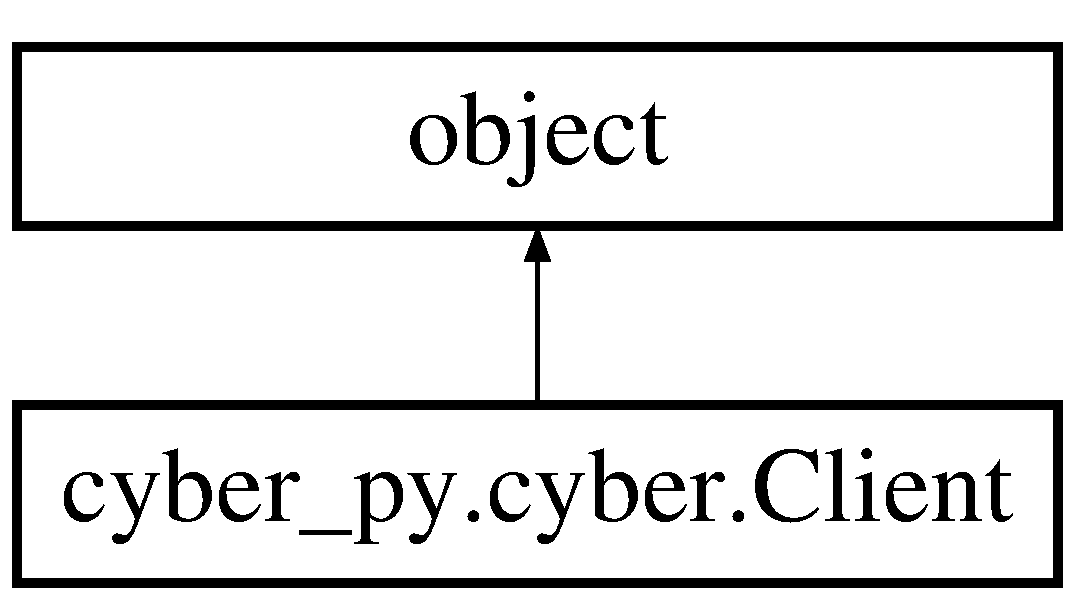
\includegraphics[height=2.000000cm]{classcyber__py_1_1cyber_1_1Client}
\end{center}
\end{figure}
\subsection*{Public Member Functions}
\begin{DoxyCompactItemize}
\item 
def \hyperlink{classcyber__py_1_1cyber_1_1Client_ab3122d6810002464fb74e97619894333}{\-\_\-\-\_\-init\-\_\-\-\_\-}
\item 
def \hyperlink{classcyber__py_1_1cyber_1_1Client_a9e7110cbfe2c5abd6d7821f17fbba4ab}{send\-\_\-request}
\end{DoxyCompactItemize}
\subsection*{Public Attributes}
\begin{DoxyCompactItemize}
\item 
\hyperlink{classcyber__py_1_1cyber_1_1Client_a10e86dbb94c8268317dda6736d082b9e}{client}
\item 
\hyperlink{classcyber__py_1_1cyber_1_1Client_ac47309e59a536f1906adea30181e2562}{data\-\_\-type}
\end{DoxyCompactItemize}


\subsection{Detailed Description}
\begin{DoxyVerb}Class for cyber service client wrapper.
\end{DoxyVerb}
 

\subsection{Constructor \& Destructor Documentation}
\hypertarget{classcyber__py_1_1cyber_1_1Client_ab3122d6810002464fb74e97619894333}{\index{cyber\-\_\-py\-::cyber\-::\-Client@{cyber\-\_\-py\-::cyber\-::\-Client}!\-\_\-\-\_\-init\-\_\-\-\_\-@{\-\_\-\-\_\-init\-\_\-\-\_\-}}
\index{\-\_\-\-\_\-init\-\_\-\-\_\-@{\-\_\-\-\_\-init\-\_\-\-\_\-}!cyber_py::cyber::Client@{cyber\-\_\-py\-::cyber\-::\-Client}}
\subsubsection[{\-\_\-\-\_\-init\-\_\-\-\_\-}]{\setlength{\rightskip}{0pt plus 5cm}def cyber\-\_\-py.\-cyber.\-Client.\-\_\-\-\_\-init\-\_\-\-\_\- (
\begin{DoxyParamCaption}
\item[{}]{self, }
\item[{}]{client, }
\item[{}]{data\-\_\-type}
\end{DoxyParamCaption}
)}}\label{classcyber__py_1_1cyber_1_1Client_ab3122d6810002464fb74e97619894333}


\subsection{Member Function Documentation}
\hypertarget{classcyber__py_1_1cyber_1_1Client_a9e7110cbfe2c5abd6d7821f17fbba4ab}{\index{cyber\-\_\-py\-::cyber\-::\-Client@{cyber\-\_\-py\-::cyber\-::\-Client}!send\-\_\-request@{send\-\_\-request}}
\index{send\-\_\-request@{send\-\_\-request}!cyber_py::cyber::Client@{cyber\-\_\-py\-::cyber\-::\-Client}}
\subsubsection[{send\-\_\-request}]{\setlength{\rightskip}{0pt plus 5cm}def cyber\-\_\-py.\-cyber.\-Client.\-send\-\_\-request (
\begin{DoxyParamCaption}
\item[{}]{self, }
\item[{}]{data}
\end{DoxyParamCaption}
)}}\label{classcyber__py_1_1cyber_1_1Client_a9e7110cbfe2c5abd6d7821f17fbba4ab}
\begin{DoxyVerb}send request to service
@param self
@param data: proto message to send
@return : None or response
\end{DoxyVerb}
 

\subsection{Member Data Documentation}
\hypertarget{classcyber__py_1_1cyber_1_1Client_a10e86dbb94c8268317dda6736d082b9e}{\index{cyber\-\_\-py\-::cyber\-::\-Client@{cyber\-\_\-py\-::cyber\-::\-Client}!client@{client}}
\index{client@{client}!cyber_py::cyber::Client@{cyber\-\_\-py\-::cyber\-::\-Client}}
\subsubsection[{client}]{\setlength{\rightskip}{0pt plus 5cm}cyber\-\_\-py.\-cyber.\-Client.\-client}}\label{classcyber__py_1_1cyber_1_1Client_a10e86dbb94c8268317dda6736d082b9e}
\hypertarget{classcyber__py_1_1cyber_1_1Client_ac47309e59a536f1906adea30181e2562}{\index{cyber\-\_\-py\-::cyber\-::\-Client@{cyber\-\_\-py\-::cyber\-::\-Client}!data\-\_\-type@{data\-\_\-type}}
\index{data\-\_\-type@{data\-\_\-type}!cyber_py::cyber::Client@{cyber\-\_\-py\-::cyber\-::\-Client}}
\subsubsection[{data\-\_\-type}]{\setlength{\rightskip}{0pt plus 5cm}cyber\-\_\-py.\-cyber.\-Client.\-data\-\_\-type}}\label{classcyber__py_1_1cyber_1_1Client_ac47309e59a536f1906adea30181e2562}


The documentation for this class was generated from the following file\-:\begin{DoxyCompactItemize}
\item 
python/cyber\-\_\-py/\hyperlink{cyber_8py}{cyber.\-py}\end{DoxyCompactItemize}

\hypertarget{classcyber__py_1_1cyber__time_1_1Duration}{\section{cyber\-\_\-py.\-cyber\-\_\-time.\-Duration Class Reference}
\label{classcyber__py_1_1cyber__time_1_1Duration}\index{cyber\-\_\-py.\-cyber\-\_\-time.\-Duration@{cyber\-\_\-py.\-cyber\-\_\-time.\-Duration}}
}
Inheritance diagram for cyber\-\_\-py.\-cyber\-\_\-time.\-Duration\-:\begin{figure}[H]
\begin{center}
\leavevmode
\includegraphics[height=2.000000cm]{classcyber__py_1_1cyber__time_1_1Duration}
\end{center}
\end{figure}
\subsection*{Public Member Functions}
\begin{DoxyCompactItemize}
\item 
def \hyperlink{classcyber__py_1_1cyber__time_1_1Duration_a08565e30a168564babacbf88550df9b5}{\-\_\-\-\_\-init\-\_\-\-\_\-}
\item 
def \hyperlink{classcyber__py_1_1cyber__time_1_1Duration_aec663fca7762f1343902eda1a13843ea}{\-\_\-\-\_\-del\-\_\-\-\_\-}
\item 
def \hyperlink{classcyber__py_1_1cyber__time_1_1Duration_af9c3391683f8d3c6a1c1850c31aa3b83}{sleep}
\item 
def \hyperlink{classcyber__py_1_1cyber__time_1_1Duration_a5d1da6e53fad943b6d47f25fe2e9d93a}{\-\_\-\-\_\-str\-\_\-\-\_\-}
\item 
def \hyperlink{classcyber__py_1_1cyber__time_1_1Duration_a05685d23f3a6ee64cbffcb2264a2641c}{to\-\_\-sec}
\item 
def \hyperlink{classcyber__py_1_1cyber__time_1_1Duration_a6af1ecab94c554db69f8c19196ad3d49}{to\-\_\-nsec}
\item 
def \hyperlink{classcyber__py_1_1cyber__time_1_1Duration_a16c36cf42d30517232088bedb5ddef7d}{iszero}
\item 
def \hyperlink{classcyber__py_1_1cyber__time_1_1Duration_a7aaf4ec01986982cd51fe1ed482269c1}{\-\_\-\-\_\-add\-\_\-\-\_\-}
\item 
def \hyperlink{classcyber__py_1_1cyber__time_1_1Duration_ab7e6d0b5e6a1e45f4606651e598323fa}{\-\_\-\-\_\-radd\-\_\-\-\_\-}
\item 
def \hyperlink{classcyber__py_1_1cyber__time_1_1Duration_a6a5276bb0333ce402698d77130e33c2d}{\-\_\-\-\_\-sub\-\_\-\-\_\-}
\item 
def \hyperlink{classcyber__py_1_1cyber__time_1_1Duration_ab591c069f725358676fffa4ac52a8530}{\-\_\-\-\_\-lt\-\_\-\-\_\-}
\item 
def \hyperlink{classcyber__py_1_1cyber__time_1_1Duration_ab4335bbfd55672f8ac20c2f1ea1f7fa5}{\-\_\-\-\_\-gt\-\_\-\-\_\-}
\item 
def \hyperlink{classcyber__py_1_1cyber__time_1_1Duration_aca5d7aad25c073f58d7f774e491f7ea4}{\-\_\-\-\_\-le\-\_\-\-\_\-}
\item 
def \hyperlink{classcyber__py_1_1cyber__time_1_1Duration_ab09a3f314504a602e35b748e8e47e7d9}{\-\_\-\-\_\-ge\-\_\-\-\_\-}
\item 
def \hyperlink{classcyber__py_1_1cyber__time_1_1Duration_af62889ca6bcea88a6d38ec9d4c7c1631}{\-\_\-\-\_\-eq\-\_\-\-\_\-}
\item 
def \hyperlink{classcyber__py_1_1cyber__time_1_1Duration_a641308cf22a8f5d49989c43c9648d443}{\-\_\-\-\_\-ne\-\_\-\-\_\-}
\end{DoxyCompactItemize}
\subsection*{Public Attributes}
\begin{DoxyCompactItemize}
\item 
\hyperlink{classcyber__py_1_1cyber__time_1_1Duration_acc9cd4d365707e296573ec88b0150d11}{nanoseconds\-\_\-}
\item 
\hyperlink{classcyber__py_1_1cyber__time_1_1Duration_abc7dca6e0a9cf8e6f336e2b5a7e9fac3}{duration\-\_\-}
\end{DoxyCompactItemize}


\subsection{Detailed Description}
\begin{DoxyVerb}Class for cyber Duration wrapper.
\end{DoxyVerb}
 

\subsection{Constructor \& Destructor Documentation}
\hypertarget{classcyber__py_1_1cyber__time_1_1Duration_a08565e30a168564babacbf88550df9b5}{\index{cyber\-\_\-py\-::cyber\-\_\-time\-::\-Duration@{cyber\-\_\-py\-::cyber\-\_\-time\-::\-Duration}!\-\_\-\-\_\-init\-\_\-\-\_\-@{\-\_\-\-\_\-init\-\_\-\-\_\-}}
\index{\-\_\-\-\_\-init\-\_\-\-\_\-@{\-\_\-\-\_\-init\-\_\-\-\_\-}!cyber_py::cyber_time::Duration@{cyber\-\_\-py\-::cyber\-\_\-time\-::\-Duration}}
\subsubsection[{\-\_\-\-\_\-init\-\_\-\-\_\-}]{\setlength{\rightskip}{0pt plus 5cm}def cyber\-\_\-py.\-cyber\-\_\-time.\-Duration.\-\_\-\-\_\-init\-\_\-\-\_\- (
\begin{DoxyParamCaption}
\item[{}]{self, }
\item[{}]{other}
\end{DoxyParamCaption}
)}}\label{classcyber__py_1_1cyber__time_1_1Duration_a08565e30a168564babacbf88550df9b5}
\hypertarget{classcyber__py_1_1cyber__time_1_1Duration_aec663fca7762f1343902eda1a13843ea}{\index{cyber\-\_\-py\-::cyber\-\_\-time\-::\-Duration@{cyber\-\_\-py\-::cyber\-\_\-time\-::\-Duration}!\-\_\-\-\_\-del\-\_\-\-\_\-@{\-\_\-\-\_\-del\-\_\-\-\_\-}}
\index{\-\_\-\-\_\-del\-\_\-\-\_\-@{\-\_\-\-\_\-del\-\_\-\-\_\-}!cyber_py::cyber_time::Duration@{cyber\-\_\-py\-::cyber\-\_\-time\-::\-Duration}}
\subsubsection[{\-\_\-\-\_\-del\-\_\-\-\_\-}]{\setlength{\rightskip}{0pt plus 5cm}def cyber\-\_\-py.\-cyber\-\_\-time.\-Duration.\-\_\-\-\_\-del\-\_\-\-\_\- (
\begin{DoxyParamCaption}
\item[{}]{self}
\end{DoxyParamCaption}
)}}\label{classcyber__py_1_1cyber__time_1_1Duration_aec663fca7762f1343902eda1a13843ea}


\subsection{Member Function Documentation}
\hypertarget{classcyber__py_1_1cyber__time_1_1Duration_a7aaf4ec01986982cd51fe1ed482269c1}{\index{cyber\-\_\-py\-::cyber\-\_\-time\-::\-Duration@{cyber\-\_\-py\-::cyber\-\_\-time\-::\-Duration}!\-\_\-\-\_\-add\-\_\-\-\_\-@{\-\_\-\-\_\-add\-\_\-\-\_\-}}
\index{\-\_\-\-\_\-add\-\_\-\-\_\-@{\-\_\-\-\_\-add\-\_\-\-\_\-}!cyber_py::cyber_time::Duration@{cyber\-\_\-py\-::cyber\-\_\-time\-::\-Duration}}
\subsubsection[{\-\_\-\-\_\-add\-\_\-\-\_\-}]{\setlength{\rightskip}{0pt plus 5cm}def cyber\-\_\-py.\-cyber\-\_\-time.\-Duration.\-\_\-\-\_\-add\-\_\-\-\_\- (
\begin{DoxyParamCaption}
\item[{}]{self, }
\item[{}]{other}
\end{DoxyParamCaption}
)}}\label{classcyber__py_1_1cyber__time_1_1Duration_a7aaf4ec01986982cd51fe1ed482269c1}
\hypertarget{classcyber__py_1_1cyber__time_1_1Duration_af62889ca6bcea88a6d38ec9d4c7c1631}{\index{cyber\-\_\-py\-::cyber\-\_\-time\-::\-Duration@{cyber\-\_\-py\-::cyber\-\_\-time\-::\-Duration}!\-\_\-\-\_\-eq\-\_\-\-\_\-@{\-\_\-\-\_\-eq\-\_\-\-\_\-}}
\index{\-\_\-\-\_\-eq\-\_\-\-\_\-@{\-\_\-\-\_\-eq\-\_\-\-\_\-}!cyber_py::cyber_time::Duration@{cyber\-\_\-py\-::cyber\-\_\-time\-::\-Duration}}
\subsubsection[{\-\_\-\-\_\-eq\-\_\-\-\_\-}]{\setlength{\rightskip}{0pt plus 5cm}def cyber\-\_\-py.\-cyber\-\_\-time.\-Duration.\-\_\-\-\_\-eq\-\_\-\-\_\- (
\begin{DoxyParamCaption}
\item[{}]{self, }
\item[{}]{other}
\end{DoxyParamCaption}
)}}\label{classcyber__py_1_1cyber__time_1_1Duration_af62889ca6bcea88a6d38ec9d4c7c1631}
\hypertarget{classcyber__py_1_1cyber__time_1_1Duration_ab09a3f314504a602e35b748e8e47e7d9}{\index{cyber\-\_\-py\-::cyber\-\_\-time\-::\-Duration@{cyber\-\_\-py\-::cyber\-\_\-time\-::\-Duration}!\-\_\-\-\_\-ge\-\_\-\-\_\-@{\-\_\-\-\_\-ge\-\_\-\-\_\-}}
\index{\-\_\-\-\_\-ge\-\_\-\-\_\-@{\-\_\-\-\_\-ge\-\_\-\-\_\-}!cyber_py::cyber_time::Duration@{cyber\-\_\-py\-::cyber\-\_\-time\-::\-Duration}}
\subsubsection[{\-\_\-\-\_\-ge\-\_\-\-\_\-}]{\setlength{\rightskip}{0pt plus 5cm}def cyber\-\_\-py.\-cyber\-\_\-time.\-Duration.\-\_\-\-\_\-ge\-\_\-\-\_\- (
\begin{DoxyParamCaption}
\item[{}]{self, }
\item[{}]{other}
\end{DoxyParamCaption}
)}}\label{classcyber__py_1_1cyber__time_1_1Duration_ab09a3f314504a602e35b748e8e47e7d9}
\hypertarget{classcyber__py_1_1cyber__time_1_1Duration_ab4335bbfd55672f8ac20c2f1ea1f7fa5}{\index{cyber\-\_\-py\-::cyber\-\_\-time\-::\-Duration@{cyber\-\_\-py\-::cyber\-\_\-time\-::\-Duration}!\-\_\-\-\_\-gt\-\_\-\-\_\-@{\-\_\-\-\_\-gt\-\_\-\-\_\-}}
\index{\-\_\-\-\_\-gt\-\_\-\-\_\-@{\-\_\-\-\_\-gt\-\_\-\-\_\-}!cyber_py::cyber_time::Duration@{cyber\-\_\-py\-::cyber\-\_\-time\-::\-Duration}}
\subsubsection[{\-\_\-\-\_\-gt\-\_\-\-\_\-}]{\setlength{\rightskip}{0pt plus 5cm}def cyber\-\_\-py.\-cyber\-\_\-time.\-Duration.\-\_\-\-\_\-gt\-\_\-\-\_\- (
\begin{DoxyParamCaption}
\item[{}]{self, }
\item[{}]{other}
\end{DoxyParamCaption}
)}}\label{classcyber__py_1_1cyber__time_1_1Duration_ab4335bbfd55672f8ac20c2f1ea1f7fa5}
\hypertarget{classcyber__py_1_1cyber__time_1_1Duration_aca5d7aad25c073f58d7f774e491f7ea4}{\index{cyber\-\_\-py\-::cyber\-\_\-time\-::\-Duration@{cyber\-\_\-py\-::cyber\-\_\-time\-::\-Duration}!\-\_\-\-\_\-le\-\_\-\-\_\-@{\-\_\-\-\_\-le\-\_\-\-\_\-}}
\index{\-\_\-\-\_\-le\-\_\-\-\_\-@{\-\_\-\-\_\-le\-\_\-\-\_\-}!cyber_py::cyber_time::Duration@{cyber\-\_\-py\-::cyber\-\_\-time\-::\-Duration}}
\subsubsection[{\-\_\-\-\_\-le\-\_\-\-\_\-}]{\setlength{\rightskip}{0pt plus 5cm}def cyber\-\_\-py.\-cyber\-\_\-time.\-Duration.\-\_\-\-\_\-le\-\_\-\-\_\- (
\begin{DoxyParamCaption}
\item[{}]{self, }
\item[{}]{other}
\end{DoxyParamCaption}
)}}\label{classcyber__py_1_1cyber__time_1_1Duration_aca5d7aad25c073f58d7f774e491f7ea4}
\hypertarget{classcyber__py_1_1cyber__time_1_1Duration_ab591c069f725358676fffa4ac52a8530}{\index{cyber\-\_\-py\-::cyber\-\_\-time\-::\-Duration@{cyber\-\_\-py\-::cyber\-\_\-time\-::\-Duration}!\-\_\-\-\_\-lt\-\_\-\-\_\-@{\-\_\-\-\_\-lt\-\_\-\-\_\-}}
\index{\-\_\-\-\_\-lt\-\_\-\-\_\-@{\-\_\-\-\_\-lt\-\_\-\-\_\-}!cyber_py::cyber_time::Duration@{cyber\-\_\-py\-::cyber\-\_\-time\-::\-Duration}}
\subsubsection[{\-\_\-\-\_\-lt\-\_\-\-\_\-}]{\setlength{\rightskip}{0pt plus 5cm}def cyber\-\_\-py.\-cyber\-\_\-time.\-Duration.\-\_\-\-\_\-lt\-\_\-\-\_\- (
\begin{DoxyParamCaption}
\item[{}]{self, }
\item[{}]{other}
\end{DoxyParamCaption}
)}}\label{classcyber__py_1_1cyber__time_1_1Duration_ab591c069f725358676fffa4ac52a8530}
\hypertarget{classcyber__py_1_1cyber__time_1_1Duration_a641308cf22a8f5d49989c43c9648d443}{\index{cyber\-\_\-py\-::cyber\-\_\-time\-::\-Duration@{cyber\-\_\-py\-::cyber\-\_\-time\-::\-Duration}!\-\_\-\-\_\-ne\-\_\-\-\_\-@{\-\_\-\-\_\-ne\-\_\-\-\_\-}}
\index{\-\_\-\-\_\-ne\-\_\-\-\_\-@{\-\_\-\-\_\-ne\-\_\-\-\_\-}!cyber_py::cyber_time::Duration@{cyber\-\_\-py\-::cyber\-\_\-time\-::\-Duration}}
\subsubsection[{\-\_\-\-\_\-ne\-\_\-\-\_\-}]{\setlength{\rightskip}{0pt plus 5cm}def cyber\-\_\-py.\-cyber\-\_\-time.\-Duration.\-\_\-\-\_\-ne\-\_\-\-\_\- (
\begin{DoxyParamCaption}
\item[{}]{self, }
\item[{}]{other}
\end{DoxyParamCaption}
)}}\label{classcyber__py_1_1cyber__time_1_1Duration_a641308cf22a8f5d49989c43c9648d443}
\hypertarget{classcyber__py_1_1cyber__time_1_1Duration_ab7e6d0b5e6a1e45f4606651e598323fa}{\index{cyber\-\_\-py\-::cyber\-\_\-time\-::\-Duration@{cyber\-\_\-py\-::cyber\-\_\-time\-::\-Duration}!\-\_\-\-\_\-radd\-\_\-\-\_\-@{\-\_\-\-\_\-radd\-\_\-\-\_\-}}
\index{\-\_\-\-\_\-radd\-\_\-\-\_\-@{\-\_\-\-\_\-radd\-\_\-\-\_\-}!cyber_py::cyber_time::Duration@{cyber\-\_\-py\-::cyber\-\_\-time\-::\-Duration}}
\subsubsection[{\-\_\-\-\_\-radd\-\_\-\-\_\-}]{\setlength{\rightskip}{0pt plus 5cm}def cyber\-\_\-py.\-cyber\-\_\-time.\-Duration.\-\_\-\-\_\-radd\-\_\-\-\_\- (
\begin{DoxyParamCaption}
\item[{}]{self, }
\item[{}]{other}
\end{DoxyParamCaption}
)}}\label{classcyber__py_1_1cyber__time_1_1Duration_ab7e6d0b5e6a1e45f4606651e598323fa}
\hypertarget{classcyber__py_1_1cyber__time_1_1Duration_a5d1da6e53fad943b6d47f25fe2e9d93a}{\index{cyber\-\_\-py\-::cyber\-\_\-time\-::\-Duration@{cyber\-\_\-py\-::cyber\-\_\-time\-::\-Duration}!\-\_\-\-\_\-str\-\_\-\-\_\-@{\-\_\-\-\_\-str\-\_\-\-\_\-}}
\index{\-\_\-\-\_\-str\-\_\-\-\_\-@{\-\_\-\-\_\-str\-\_\-\-\_\-}!cyber_py::cyber_time::Duration@{cyber\-\_\-py\-::cyber\-\_\-time\-::\-Duration}}
\subsubsection[{\-\_\-\-\_\-str\-\_\-\-\_\-}]{\setlength{\rightskip}{0pt plus 5cm}def cyber\-\_\-py.\-cyber\-\_\-time.\-Duration.\-\_\-\-\_\-str\-\_\-\-\_\- (
\begin{DoxyParamCaption}
\item[{}]{self}
\end{DoxyParamCaption}
)}}\label{classcyber__py_1_1cyber__time_1_1Duration_a5d1da6e53fad943b6d47f25fe2e9d93a}
\hypertarget{classcyber__py_1_1cyber__time_1_1Duration_a6a5276bb0333ce402698d77130e33c2d}{\index{cyber\-\_\-py\-::cyber\-\_\-time\-::\-Duration@{cyber\-\_\-py\-::cyber\-\_\-time\-::\-Duration}!\-\_\-\-\_\-sub\-\_\-\-\_\-@{\-\_\-\-\_\-sub\-\_\-\-\_\-}}
\index{\-\_\-\-\_\-sub\-\_\-\-\_\-@{\-\_\-\-\_\-sub\-\_\-\-\_\-}!cyber_py::cyber_time::Duration@{cyber\-\_\-py\-::cyber\-\_\-time\-::\-Duration}}
\subsubsection[{\-\_\-\-\_\-sub\-\_\-\-\_\-}]{\setlength{\rightskip}{0pt plus 5cm}def cyber\-\_\-py.\-cyber\-\_\-time.\-Duration.\-\_\-\-\_\-sub\-\_\-\-\_\- (
\begin{DoxyParamCaption}
\item[{}]{self, }
\item[{}]{other}
\end{DoxyParamCaption}
)}}\label{classcyber__py_1_1cyber__time_1_1Duration_a6a5276bb0333ce402698d77130e33c2d}
\hypertarget{classcyber__py_1_1cyber__time_1_1Duration_a16c36cf42d30517232088bedb5ddef7d}{\index{cyber\-\_\-py\-::cyber\-\_\-time\-::\-Duration@{cyber\-\_\-py\-::cyber\-\_\-time\-::\-Duration}!iszero@{iszero}}
\index{iszero@{iszero}!cyber_py::cyber_time::Duration@{cyber\-\_\-py\-::cyber\-\_\-time\-::\-Duration}}
\subsubsection[{iszero}]{\setlength{\rightskip}{0pt plus 5cm}def cyber\-\_\-py.\-cyber\-\_\-time.\-Duration.\-iszero (
\begin{DoxyParamCaption}
\item[{}]{self}
\end{DoxyParamCaption}
)}}\label{classcyber__py_1_1cyber__time_1_1Duration_a16c36cf42d30517232088bedb5ddef7d}
\hypertarget{classcyber__py_1_1cyber__time_1_1Duration_af9c3391683f8d3c6a1c1850c31aa3b83}{\index{cyber\-\_\-py\-::cyber\-\_\-time\-::\-Duration@{cyber\-\_\-py\-::cyber\-\_\-time\-::\-Duration}!sleep@{sleep}}
\index{sleep@{sleep}!cyber_py::cyber_time::Duration@{cyber\-\_\-py\-::cyber\-\_\-time\-::\-Duration}}
\subsubsection[{sleep}]{\setlength{\rightskip}{0pt plus 5cm}def cyber\-\_\-py.\-cyber\-\_\-time.\-Duration.\-sleep (
\begin{DoxyParamCaption}
\item[{}]{self}
\end{DoxyParamCaption}
)}}\label{classcyber__py_1_1cyber__time_1_1Duration_af9c3391683f8d3c6a1c1850c31aa3b83}
\hypertarget{classcyber__py_1_1cyber__time_1_1Duration_a6af1ecab94c554db69f8c19196ad3d49}{\index{cyber\-\_\-py\-::cyber\-\_\-time\-::\-Duration@{cyber\-\_\-py\-::cyber\-\_\-time\-::\-Duration}!to\-\_\-nsec@{to\-\_\-nsec}}
\index{to\-\_\-nsec@{to\-\_\-nsec}!cyber_py::cyber_time::Duration@{cyber\-\_\-py\-::cyber\-\_\-time\-::\-Duration}}
\subsubsection[{to\-\_\-nsec}]{\setlength{\rightskip}{0pt plus 5cm}def cyber\-\_\-py.\-cyber\-\_\-time.\-Duration.\-to\-\_\-nsec (
\begin{DoxyParamCaption}
\item[{}]{self}
\end{DoxyParamCaption}
)}}\label{classcyber__py_1_1cyber__time_1_1Duration_a6af1ecab94c554db69f8c19196ad3d49}
\hypertarget{classcyber__py_1_1cyber__time_1_1Duration_a05685d23f3a6ee64cbffcb2264a2641c}{\index{cyber\-\_\-py\-::cyber\-\_\-time\-::\-Duration@{cyber\-\_\-py\-::cyber\-\_\-time\-::\-Duration}!to\-\_\-sec@{to\-\_\-sec}}
\index{to\-\_\-sec@{to\-\_\-sec}!cyber_py::cyber_time::Duration@{cyber\-\_\-py\-::cyber\-\_\-time\-::\-Duration}}
\subsubsection[{to\-\_\-sec}]{\setlength{\rightskip}{0pt plus 5cm}def cyber\-\_\-py.\-cyber\-\_\-time.\-Duration.\-to\-\_\-sec (
\begin{DoxyParamCaption}
\item[{}]{self}
\end{DoxyParamCaption}
)}}\label{classcyber__py_1_1cyber__time_1_1Duration_a05685d23f3a6ee64cbffcb2264a2641c}


\subsection{Member Data Documentation}
\hypertarget{classcyber__py_1_1cyber__time_1_1Duration_abc7dca6e0a9cf8e6f336e2b5a7e9fac3}{\index{cyber\-\_\-py\-::cyber\-\_\-time\-::\-Duration@{cyber\-\_\-py\-::cyber\-\_\-time\-::\-Duration}!duration\-\_\-@{duration\-\_\-}}
\index{duration\-\_\-@{duration\-\_\-}!cyber_py::cyber_time::Duration@{cyber\-\_\-py\-::cyber\-\_\-time\-::\-Duration}}
\subsubsection[{duration\-\_\-}]{\setlength{\rightskip}{0pt plus 5cm}cyber\-\_\-py.\-cyber\-\_\-time.\-Duration.\-duration\-\_\-}}\label{classcyber__py_1_1cyber__time_1_1Duration_abc7dca6e0a9cf8e6f336e2b5a7e9fac3}
\hypertarget{classcyber__py_1_1cyber__time_1_1Duration_acc9cd4d365707e296573ec88b0150d11}{\index{cyber\-\_\-py\-::cyber\-\_\-time\-::\-Duration@{cyber\-\_\-py\-::cyber\-\_\-time\-::\-Duration}!nanoseconds\-\_\-@{nanoseconds\-\_\-}}
\index{nanoseconds\-\_\-@{nanoseconds\-\_\-}!cyber_py::cyber_time::Duration@{cyber\-\_\-py\-::cyber\-\_\-time\-::\-Duration}}
\subsubsection[{nanoseconds\-\_\-}]{\setlength{\rightskip}{0pt plus 5cm}cyber\-\_\-py.\-cyber\-\_\-time.\-Duration.\-nanoseconds\-\_\-}}\label{classcyber__py_1_1cyber__time_1_1Duration_acc9cd4d365707e296573ec88b0150d11}


The documentation for this class was generated from the following file\-:\begin{DoxyCompactItemize}
\item 
python/cyber\-\_\-py/\hyperlink{cyber__time_8py}{cyber\-\_\-time.\-py}\end{DoxyCompactItemize}

\hypertarget{classcyber__py_1_1cyber_1_1Node}{\section{cyber\-\_\-py.\-cyber.\-Node Class Reference}
\label{classcyber__py_1_1cyber_1_1Node}\index{cyber\-\_\-py.\-cyber.\-Node@{cyber\-\_\-py.\-cyber.\-Node}}
}
Inheritance diagram for cyber\-\_\-py.\-cyber.\-Node\-:\begin{figure}[H]
\begin{center}
\leavevmode
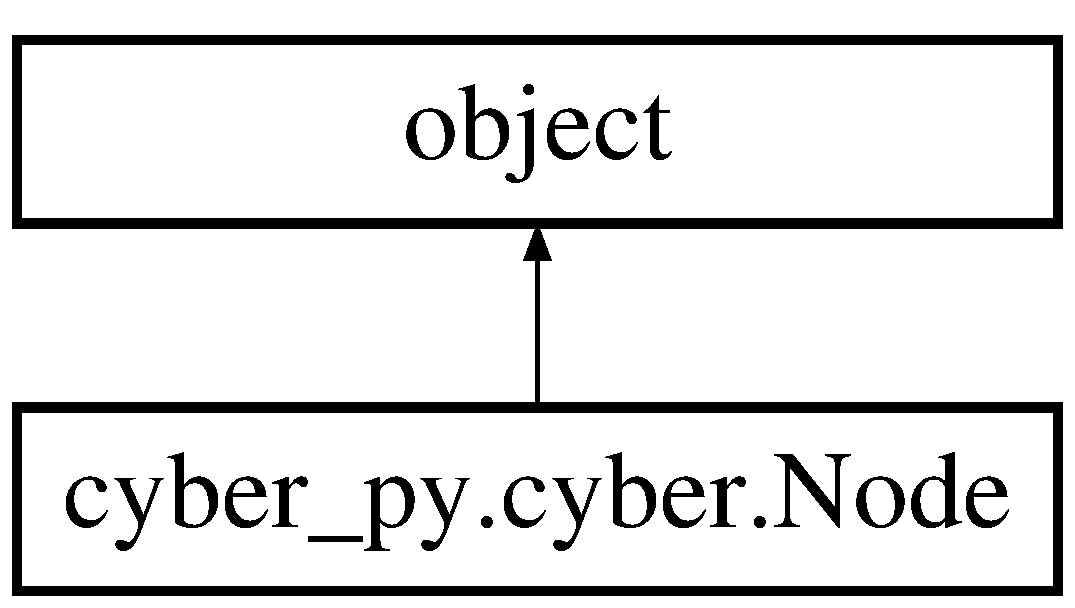
\includegraphics[height=2.000000cm]{classcyber__py_1_1cyber_1_1Node}
\end{center}
\end{figure}
\subsection*{Public Member Functions}
\begin{DoxyCompactItemize}
\item 
def \hyperlink{classcyber__py_1_1cyber_1_1Node_a7ed5cbe9188a3e758e9e3d25ac375d7c}{\-\_\-\-\_\-init\-\_\-\-\_\-}
\item 
def \hyperlink{classcyber__py_1_1cyber_1_1Node_ab458e2836cf1ddff40e94b9ac4552da2}{\-\_\-\-\_\-del\-\_\-\-\_\-}
\item 
def \hyperlink{classcyber__py_1_1cyber_1_1Node_a114d1b9766de4aa0d51507e3f15896ec}{register\-\_\-message}
\item 
def \hyperlink{classcyber__py_1_1cyber_1_1Node_a04929ca39d6ab0a6ce9a7464da05bdf4}{create\-\_\-writer}
\item 
def \hyperlink{classcyber__py_1_1cyber_1_1Node_aeb4ffff77bb79bed4c88c2f339dc354b}{reader\-\_\-callback}
\item 
def \hyperlink{classcyber__py_1_1cyber_1_1Node_ae688186c7437c468d97200d1c8e6c461}{create\-\_\-reader}
\item 
def \hyperlink{classcyber__py_1_1cyber_1_1Node_a66ba57a5a8eeeb7a3951e278d59dc73b}{create\-\_\-client}
\item 
def \hyperlink{classcyber__py_1_1cyber_1_1Node_a83d825faba3823b920a8351639819d7a}{service\-\_\-callback}
\item 
def \hyperlink{classcyber__py_1_1cyber_1_1Node_a462c5baf7e7865e3748444f9bc25d1a3}{create\-\_\-service}
\item 
def \hyperlink{classcyber__py_1_1cyber_1_1Node_aa84f141f87c59573e91b7e475eda24cb}{spin}
\end{DoxyCompactItemize}
\subsection*{Public Attributes}
\begin{DoxyCompactItemize}
\item 
\hyperlink{classcyber__py_1_1cyber_1_1Node_af1d1465e7e1306766e7e6e6f68126365}{node}
\item 
\hyperlink{classcyber__py_1_1cyber_1_1Node_afe737c18cc7236c5121efd49400c09ab}{list\-\_\-writer}
\item 
\hyperlink{classcyber__py_1_1cyber_1_1Node_a44dc5de2dbefff08ad9bb54cabe0a9e2}{list\-\_\-reader}
\item 
\hyperlink{classcyber__py_1_1cyber_1_1Node_aeec0921d80a2daeffe5f00df5b058532}{subs}
\item 
\hyperlink{classcyber__py_1_1cyber_1_1Node_a8f7d27e8c698ada3083a3c7074ced956}{pubs}
\item 
\hyperlink{classcyber__py_1_1cyber_1_1Node_a0f6052c868b842325fde215a09f75363}{list\-\_\-client}
\item 
\hyperlink{classcyber__py_1_1cyber_1_1Node_a5e8e78b807876e508fd5211006ec7c31}{list\-\_\-service}
\item 
\hyperlink{classcyber__py_1_1cyber_1_1Node_a4d7844d57accfe33f50304335ad065f5}{mutex}
\item 
\hyperlink{classcyber__py_1_1cyber_1_1Node_a619cab27f7ec745edf0f06d2cd3aa630}{callbacks}
\item 
\hyperlink{classcyber__py_1_1cyber_1_1Node_a362299aa1d91ea7e0e557858b3c0b826}{services}
\end{DoxyCompactItemize}


\subsection{Detailed Description}
\begin{DoxyVerb}Class for cyber Node wrapper.
\end{DoxyVerb}
 

\subsection{Constructor \& Destructor Documentation}
\hypertarget{classcyber__py_1_1cyber_1_1Node_a7ed5cbe9188a3e758e9e3d25ac375d7c}{\index{cyber\-\_\-py\-::cyber\-::\-Node@{cyber\-\_\-py\-::cyber\-::\-Node}!\-\_\-\-\_\-init\-\_\-\-\_\-@{\-\_\-\-\_\-init\-\_\-\-\_\-}}
\index{\-\_\-\-\_\-init\-\_\-\-\_\-@{\-\_\-\-\_\-init\-\_\-\-\_\-}!cyber_py::cyber::Node@{cyber\-\_\-py\-::cyber\-::\-Node}}
\subsubsection[{\-\_\-\-\_\-init\-\_\-\-\_\-}]{\setlength{\rightskip}{0pt plus 5cm}def cyber\-\_\-py.\-cyber.\-Node.\-\_\-\-\_\-init\-\_\-\-\_\- (
\begin{DoxyParamCaption}
\item[{}]{self, }
\item[{}]{name}
\end{DoxyParamCaption}
)}}\label{classcyber__py_1_1cyber_1_1Node_a7ed5cbe9188a3e758e9e3d25ac375d7c}
\hypertarget{classcyber__py_1_1cyber_1_1Node_ab458e2836cf1ddff40e94b9ac4552da2}{\index{cyber\-\_\-py\-::cyber\-::\-Node@{cyber\-\_\-py\-::cyber\-::\-Node}!\-\_\-\-\_\-del\-\_\-\-\_\-@{\-\_\-\-\_\-del\-\_\-\-\_\-}}
\index{\-\_\-\-\_\-del\-\_\-\-\_\-@{\-\_\-\-\_\-del\-\_\-\-\_\-}!cyber_py::cyber::Node@{cyber\-\_\-py\-::cyber\-::\-Node}}
\subsubsection[{\-\_\-\-\_\-del\-\_\-\-\_\-}]{\setlength{\rightskip}{0pt plus 5cm}def cyber\-\_\-py.\-cyber.\-Node.\-\_\-\-\_\-del\-\_\-\-\_\- (
\begin{DoxyParamCaption}
\item[{}]{self}
\end{DoxyParamCaption}
)}}\label{classcyber__py_1_1cyber_1_1Node_ab458e2836cf1ddff40e94b9ac4552da2}


\subsection{Member Function Documentation}
\hypertarget{classcyber__py_1_1cyber_1_1Node_a66ba57a5a8eeeb7a3951e278d59dc73b}{\index{cyber\-\_\-py\-::cyber\-::\-Node@{cyber\-\_\-py\-::cyber\-::\-Node}!create\-\_\-client@{create\-\_\-client}}
\index{create\-\_\-client@{create\-\_\-client}!cyber_py::cyber::Node@{cyber\-\_\-py\-::cyber\-::\-Node}}
\subsubsection[{create\-\_\-client}]{\setlength{\rightskip}{0pt plus 5cm}def cyber\-\_\-py.\-cyber.\-Node.\-create\-\_\-client (
\begin{DoxyParamCaption}
\item[{}]{self, }
\item[{}]{name, }
\item[{}]{request\-\_\-data\-\_\-type, }
\item[{}]{response\-\_\-data\-\_\-type}
\end{DoxyParamCaption}
)}}\label{classcyber__py_1_1cyber_1_1Node_a66ba57a5a8eeeb7a3951e278d59dc73b}
\hypertarget{classcyber__py_1_1cyber_1_1Node_ae688186c7437c468d97200d1c8e6c461}{\index{cyber\-\_\-py\-::cyber\-::\-Node@{cyber\-\_\-py\-::cyber\-::\-Node}!create\-\_\-reader@{create\-\_\-reader}}
\index{create\-\_\-reader@{create\-\_\-reader}!cyber_py::cyber::Node@{cyber\-\_\-py\-::cyber\-::\-Node}}
\subsubsection[{create\-\_\-reader}]{\setlength{\rightskip}{0pt plus 5cm}def cyber\-\_\-py.\-cyber.\-Node.\-create\-\_\-reader (
\begin{DoxyParamCaption}
\item[{}]{self, }
\item[{}]{name, }
\item[{}]{data\-\_\-type, }
\item[{}]{callback, }
\item[{}]{args = {\ttfamily None}}
\end{DoxyParamCaption}
)}}\label{classcyber__py_1_1cyber_1_1Node_ae688186c7437c468d97200d1c8e6c461}
\begin{DoxyVerb}create a topic reader for receive message from topic.
@param self
@param name str: topic name
@param data_type proto: message class for serialization
@callback fn: function to call (fn(data)) when data is
   received. If args is set, the function must
   accept the args as a second argument,
   i.e. fn(data, args)
@args any: additional arguments to pass to the callback
\end{DoxyVerb}
 \hypertarget{classcyber__py_1_1cyber_1_1Node_a462c5baf7e7865e3748444f9bc25d1a3}{\index{cyber\-\_\-py\-::cyber\-::\-Node@{cyber\-\_\-py\-::cyber\-::\-Node}!create\-\_\-service@{create\-\_\-service}}
\index{create\-\_\-service@{create\-\_\-service}!cyber_py::cyber::Node@{cyber\-\_\-py\-::cyber\-::\-Node}}
\subsubsection[{create\-\_\-service}]{\setlength{\rightskip}{0pt plus 5cm}def cyber\-\_\-py.\-cyber.\-Node.\-create\-\_\-service (
\begin{DoxyParamCaption}
\item[{}]{self, }
\item[{}]{name, }
\item[{}]{req\-\_\-data\-\_\-type, }
\item[{}]{res\-\_\-data\-\_\-type, }
\item[{}]{callback, }
\item[{}]{args = {\ttfamily None}}
\end{DoxyParamCaption}
)}}\label{classcyber__py_1_1cyber_1_1Node_a462c5baf7e7865e3748444f9bc25d1a3}
\hypertarget{classcyber__py_1_1cyber_1_1Node_a04929ca39d6ab0a6ce9a7464da05bdf4}{\index{cyber\-\_\-py\-::cyber\-::\-Node@{cyber\-\_\-py\-::cyber\-::\-Node}!create\-\_\-writer@{create\-\_\-writer}}
\index{create\-\_\-writer@{create\-\_\-writer}!cyber_py::cyber::Node@{cyber\-\_\-py\-::cyber\-::\-Node}}
\subsubsection[{create\-\_\-writer}]{\setlength{\rightskip}{0pt plus 5cm}def cyber\-\_\-py.\-cyber.\-Node.\-create\-\_\-writer (
\begin{DoxyParamCaption}
\item[{}]{self, }
\item[{}]{name, }
\item[{}]{data\-\_\-type, }
\item[{}]{qos\-\_\-depth = {\ttfamily 1}}
\end{DoxyParamCaption}
)}}\label{classcyber__py_1_1cyber_1_1Node_a04929ca39d6ab0a6ce9a7464da05bdf4}
\begin{DoxyVerb}create a topic writer for send message to topic.
@param self
@param name str: topic name
@param data_type proto: message class for serialization
\end{DoxyVerb}
 \hypertarget{classcyber__py_1_1cyber_1_1Node_aeb4ffff77bb79bed4c88c2f339dc354b}{\index{cyber\-\_\-py\-::cyber\-::\-Node@{cyber\-\_\-py\-::cyber\-::\-Node}!reader\-\_\-callback@{reader\-\_\-callback}}
\index{reader\-\_\-callback@{reader\-\_\-callback}!cyber_py::cyber::Node@{cyber\-\_\-py\-::cyber\-::\-Node}}
\subsubsection[{reader\-\_\-callback}]{\setlength{\rightskip}{0pt plus 5cm}def cyber\-\_\-py.\-cyber.\-Node.\-reader\-\_\-callback (
\begin{DoxyParamCaption}
\item[{}]{self, }
\item[{}]{name}
\end{DoxyParamCaption}
)}}\label{classcyber__py_1_1cyber_1_1Node_aeb4ffff77bb79bed4c88c2f339dc354b}
\begin{DoxyVerb}reader callback
\end{DoxyVerb}
 \hypertarget{classcyber__py_1_1cyber_1_1Node_a114d1b9766de4aa0d51507e3f15896ec}{\index{cyber\-\_\-py\-::cyber\-::\-Node@{cyber\-\_\-py\-::cyber\-::\-Node}!register\-\_\-message@{register\-\_\-message}}
\index{register\-\_\-message@{register\-\_\-message}!cyber_py::cyber::Node@{cyber\-\_\-py\-::cyber\-::\-Node}}
\subsubsection[{register\-\_\-message}]{\setlength{\rightskip}{0pt plus 5cm}def cyber\-\_\-py.\-cyber.\-Node.\-register\-\_\-message (
\begin{DoxyParamCaption}
\item[{}]{self, }
\item[{}]{file\-\_\-desc}
\end{DoxyParamCaption}
)}}\label{classcyber__py_1_1cyber_1_1Node_a114d1b9766de4aa0d51507e3f15896ec}
\begin{DoxyVerb}register proto message desc file.
\end{DoxyVerb}
 \hypertarget{classcyber__py_1_1cyber_1_1Node_a83d825faba3823b920a8351639819d7a}{\index{cyber\-\_\-py\-::cyber\-::\-Node@{cyber\-\_\-py\-::cyber\-::\-Node}!service\-\_\-callback@{service\-\_\-callback}}
\index{service\-\_\-callback@{service\-\_\-callback}!cyber_py::cyber::Node@{cyber\-\_\-py\-::cyber\-::\-Node}}
\subsubsection[{service\-\_\-callback}]{\setlength{\rightskip}{0pt plus 5cm}def cyber\-\_\-py.\-cyber.\-Node.\-service\-\_\-callback (
\begin{DoxyParamCaption}
\item[{}]{self, }
\item[{}]{name}
\end{DoxyParamCaption}
)}}\label{classcyber__py_1_1cyber_1_1Node_a83d825faba3823b920a8351639819d7a}
\hypertarget{classcyber__py_1_1cyber_1_1Node_aa84f141f87c59573e91b7e475eda24cb}{\index{cyber\-\_\-py\-::cyber\-::\-Node@{cyber\-\_\-py\-::cyber\-::\-Node}!spin@{spin}}
\index{spin@{spin}!cyber_py::cyber::Node@{cyber\-\_\-py\-::cyber\-::\-Node}}
\subsubsection[{spin}]{\setlength{\rightskip}{0pt plus 5cm}def cyber\-\_\-py.\-cyber.\-Node.\-spin (
\begin{DoxyParamCaption}
\item[{}]{self}
\end{DoxyParamCaption}
)}}\label{classcyber__py_1_1cyber_1_1Node_aa84f141f87c59573e91b7e475eda24cb}
\begin{DoxyVerb}spin in wait and process message.
@param self
\end{DoxyVerb}
 

\subsection{Member Data Documentation}
\hypertarget{classcyber__py_1_1cyber_1_1Node_a619cab27f7ec745edf0f06d2cd3aa630}{\index{cyber\-\_\-py\-::cyber\-::\-Node@{cyber\-\_\-py\-::cyber\-::\-Node}!callbacks@{callbacks}}
\index{callbacks@{callbacks}!cyber_py::cyber::Node@{cyber\-\_\-py\-::cyber\-::\-Node}}
\subsubsection[{callbacks}]{\setlength{\rightskip}{0pt plus 5cm}cyber\-\_\-py.\-cyber.\-Node.\-callbacks}}\label{classcyber__py_1_1cyber_1_1Node_a619cab27f7ec745edf0f06d2cd3aa630}
\hypertarget{classcyber__py_1_1cyber_1_1Node_a0f6052c868b842325fde215a09f75363}{\index{cyber\-\_\-py\-::cyber\-::\-Node@{cyber\-\_\-py\-::cyber\-::\-Node}!list\-\_\-client@{list\-\_\-client}}
\index{list\-\_\-client@{list\-\_\-client}!cyber_py::cyber::Node@{cyber\-\_\-py\-::cyber\-::\-Node}}
\subsubsection[{list\-\_\-client}]{\setlength{\rightskip}{0pt plus 5cm}cyber\-\_\-py.\-cyber.\-Node.\-list\-\_\-client}}\label{classcyber__py_1_1cyber_1_1Node_a0f6052c868b842325fde215a09f75363}
\hypertarget{classcyber__py_1_1cyber_1_1Node_a44dc5de2dbefff08ad9bb54cabe0a9e2}{\index{cyber\-\_\-py\-::cyber\-::\-Node@{cyber\-\_\-py\-::cyber\-::\-Node}!list\-\_\-reader@{list\-\_\-reader}}
\index{list\-\_\-reader@{list\-\_\-reader}!cyber_py::cyber::Node@{cyber\-\_\-py\-::cyber\-::\-Node}}
\subsubsection[{list\-\_\-reader}]{\setlength{\rightskip}{0pt plus 5cm}cyber\-\_\-py.\-cyber.\-Node.\-list\-\_\-reader}}\label{classcyber__py_1_1cyber_1_1Node_a44dc5de2dbefff08ad9bb54cabe0a9e2}
\hypertarget{classcyber__py_1_1cyber_1_1Node_a5e8e78b807876e508fd5211006ec7c31}{\index{cyber\-\_\-py\-::cyber\-::\-Node@{cyber\-\_\-py\-::cyber\-::\-Node}!list\-\_\-service@{list\-\_\-service}}
\index{list\-\_\-service@{list\-\_\-service}!cyber_py::cyber::Node@{cyber\-\_\-py\-::cyber\-::\-Node}}
\subsubsection[{list\-\_\-service}]{\setlength{\rightskip}{0pt plus 5cm}cyber\-\_\-py.\-cyber.\-Node.\-list\-\_\-service}}\label{classcyber__py_1_1cyber_1_1Node_a5e8e78b807876e508fd5211006ec7c31}
\hypertarget{classcyber__py_1_1cyber_1_1Node_afe737c18cc7236c5121efd49400c09ab}{\index{cyber\-\_\-py\-::cyber\-::\-Node@{cyber\-\_\-py\-::cyber\-::\-Node}!list\-\_\-writer@{list\-\_\-writer}}
\index{list\-\_\-writer@{list\-\_\-writer}!cyber_py::cyber::Node@{cyber\-\_\-py\-::cyber\-::\-Node}}
\subsubsection[{list\-\_\-writer}]{\setlength{\rightskip}{0pt plus 5cm}cyber\-\_\-py.\-cyber.\-Node.\-list\-\_\-writer}}\label{classcyber__py_1_1cyber_1_1Node_afe737c18cc7236c5121efd49400c09ab}
\hypertarget{classcyber__py_1_1cyber_1_1Node_a4d7844d57accfe33f50304335ad065f5}{\index{cyber\-\_\-py\-::cyber\-::\-Node@{cyber\-\_\-py\-::cyber\-::\-Node}!mutex@{mutex}}
\index{mutex@{mutex}!cyber_py::cyber::Node@{cyber\-\_\-py\-::cyber\-::\-Node}}
\subsubsection[{mutex}]{\setlength{\rightskip}{0pt plus 5cm}cyber\-\_\-py.\-cyber.\-Node.\-mutex}}\label{classcyber__py_1_1cyber_1_1Node_a4d7844d57accfe33f50304335ad065f5}
\hypertarget{classcyber__py_1_1cyber_1_1Node_af1d1465e7e1306766e7e6e6f68126365}{\index{cyber\-\_\-py\-::cyber\-::\-Node@{cyber\-\_\-py\-::cyber\-::\-Node}!node@{node}}
\index{node@{node}!cyber_py::cyber::Node@{cyber\-\_\-py\-::cyber\-::\-Node}}
\subsubsection[{node}]{\setlength{\rightskip}{0pt plus 5cm}cyber\-\_\-py.\-cyber.\-Node.\-node}}\label{classcyber__py_1_1cyber_1_1Node_af1d1465e7e1306766e7e6e6f68126365}
\hypertarget{classcyber__py_1_1cyber_1_1Node_a8f7d27e8c698ada3083a3c7074ced956}{\index{cyber\-\_\-py\-::cyber\-::\-Node@{cyber\-\_\-py\-::cyber\-::\-Node}!pubs@{pubs}}
\index{pubs@{pubs}!cyber_py::cyber::Node@{cyber\-\_\-py\-::cyber\-::\-Node}}
\subsubsection[{pubs}]{\setlength{\rightskip}{0pt plus 5cm}cyber\-\_\-py.\-cyber.\-Node.\-pubs}}\label{classcyber__py_1_1cyber_1_1Node_a8f7d27e8c698ada3083a3c7074ced956}
\hypertarget{classcyber__py_1_1cyber_1_1Node_a362299aa1d91ea7e0e557858b3c0b826}{\index{cyber\-\_\-py\-::cyber\-::\-Node@{cyber\-\_\-py\-::cyber\-::\-Node}!services@{services}}
\index{services@{services}!cyber_py::cyber::Node@{cyber\-\_\-py\-::cyber\-::\-Node}}
\subsubsection[{services}]{\setlength{\rightskip}{0pt plus 5cm}cyber\-\_\-py.\-cyber.\-Node.\-services}}\label{classcyber__py_1_1cyber_1_1Node_a362299aa1d91ea7e0e557858b3c0b826}
\hypertarget{classcyber__py_1_1cyber_1_1Node_aeec0921d80a2daeffe5f00df5b058532}{\index{cyber\-\_\-py\-::cyber\-::\-Node@{cyber\-\_\-py\-::cyber\-::\-Node}!subs@{subs}}
\index{subs@{subs}!cyber_py::cyber::Node@{cyber\-\_\-py\-::cyber\-::\-Node}}
\subsubsection[{subs}]{\setlength{\rightskip}{0pt plus 5cm}cyber\-\_\-py.\-cyber.\-Node.\-subs}}\label{classcyber__py_1_1cyber_1_1Node_aeec0921d80a2daeffe5f00df5b058532}


The documentation for this class was generated from the following file\-:\begin{DoxyCompactItemize}
\item 
python/cyber\-\_\-py/\hyperlink{cyber_8py}{cyber.\-py}\end{DoxyCompactItemize}

\hypertarget{classcyber__py_1_1cyber__time_1_1Rate}{\section{cyber\-\_\-py.\-cyber\-\_\-time.\-Rate Class Reference}
\label{classcyber__py_1_1cyber__time_1_1Rate}\index{cyber\-\_\-py.\-cyber\-\_\-time.\-Rate@{cyber\-\_\-py.\-cyber\-\_\-time.\-Rate}}
}
Inheritance diagram for cyber\-\_\-py.\-cyber\-\_\-time.\-Rate\-:\begin{figure}[H]
\begin{center}
\leavevmode
\includegraphics[height=2.000000cm]{classcyber__py_1_1cyber__time_1_1Rate}
\end{center}
\end{figure}
\subsection*{Public Member Functions}
\begin{DoxyCompactItemize}
\item 
def \hyperlink{classcyber__py_1_1cyber__time_1_1Rate_a7a975548d01fcd4b340bd9c5abb69b82}{\-\_\-\-\_\-init\-\_\-\-\_\-}
\item 
def \hyperlink{classcyber__py_1_1cyber__time_1_1Rate_a84e692b9ccae558b61b927ca38f1c494}{\-\_\-\-\_\-del\-\_\-\-\_\-}
\item 
def \hyperlink{classcyber__py_1_1cyber__time_1_1Rate_a0bacd1a2c93a2957832a06fb98b85584}{\-\_\-\-\_\-str\-\_\-\-\_\-}
\item 
def \hyperlink{classcyber__py_1_1cyber__time_1_1Rate_ab7c358d86a1832ec79983619056191f7}{sleep}
\item 
def \hyperlink{classcyber__py_1_1cyber__time_1_1Rate_a9d4ca0dc8610bc59c1c222e53704f893}{reset}
\item 
def \hyperlink{classcyber__py_1_1cyber__time_1_1Rate_aefed307f8d0770546e4ba22f777a4c2b}{get\-\_\-cycle\-\_\-time}
\item 
def \hyperlink{classcyber__py_1_1cyber__time_1_1Rate_a319c3cc27b2eaa190107415c5b1ea8b4}{get\-\_\-expected\-\_\-cycle\-\_\-time}
\end{DoxyCompactItemize}
\subsection*{Public Attributes}
\begin{DoxyCompactItemize}
\item 
\hyperlink{classcyber__py_1_1cyber__time_1_1Rate_a925c7d9c5403baab034607efe37a85b9}{rate\-\_\-}
\end{DoxyCompactItemize}


\subsection{Detailed Description}
\begin{DoxyVerb}Class for cyber Rate wrapper.
\end{DoxyVerb}
 

\subsection{Constructor \& Destructor Documentation}
\hypertarget{classcyber__py_1_1cyber__time_1_1Rate_a7a975548d01fcd4b340bd9c5abb69b82}{\index{cyber\-\_\-py\-::cyber\-\_\-time\-::\-Rate@{cyber\-\_\-py\-::cyber\-\_\-time\-::\-Rate}!\-\_\-\-\_\-init\-\_\-\-\_\-@{\-\_\-\-\_\-init\-\_\-\-\_\-}}
\index{\-\_\-\-\_\-init\-\_\-\-\_\-@{\-\_\-\-\_\-init\-\_\-\-\_\-}!cyber_py::cyber_time::Rate@{cyber\-\_\-py\-::cyber\-\_\-time\-::\-Rate}}
\subsubsection[{\-\_\-\-\_\-init\-\_\-\-\_\-}]{\setlength{\rightskip}{0pt plus 5cm}def cyber\-\_\-py.\-cyber\-\_\-time.\-Rate.\-\_\-\-\_\-init\-\_\-\-\_\- (
\begin{DoxyParamCaption}
\item[{}]{self, }
\item[{}]{other}
\end{DoxyParamCaption}
)}}\label{classcyber__py_1_1cyber__time_1_1Rate_a7a975548d01fcd4b340bd9c5abb69b82}
\hypertarget{classcyber__py_1_1cyber__time_1_1Rate_a84e692b9ccae558b61b927ca38f1c494}{\index{cyber\-\_\-py\-::cyber\-\_\-time\-::\-Rate@{cyber\-\_\-py\-::cyber\-\_\-time\-::\-Rate}!\-\_\-\-\_\-del\-\_\-\-\_\-@{\-\_\-\-\_\-del\-\_\-\-\_\-}}
\index{\-\_\-\-\_\-del\-\_\-\-\_\-@{\-\_\-\-\_\-del\-\_\-\-\_\-}!cyber_py::cyber_time::Rate@{cyber\-\_\-py\-::cyber\-\_\-time\-::\-Rate}}
\subsubsection[{\-\_\-\-\_\-del\-\_\-\-\_\-}]{\setlength{\rightskip}{0pt plus 5cm}def cyber\-\_\-py.\-cyber\-\_\-time.\-Rate.\-\_\-\-\_\-del\-\_\-\-\_\- (
\begin{DoxyParamCaption}
\item[{}]{self}
\end{DoxyParamCaption}
)}}\label{classcyber__py_1_1cyber__time_1_1Rate_a84e692b9ccae558b61b927ca38f1c494}


\subsection{Member Function Documentation}
\hypertarget{classcyber__py_1_1cyber__time_1_1Rate_a0bacd1a2c93a2957832a06fb98b85584}{\index{cyber\-\_\-py\-::cyber\-\_\-time\-::\-Rate@{cyber\-\_\-py\-::cyber\-\_\-time\-::\-Rate}!\-\_\-\-\_\-str\-\_\-\-\_\-@{\-\_\-\-\_\-str\-\_\-\-\_\-}}
\index{\-\_\-\-\_\-str\-\_\-\-\_\-@{\-\_\-\-\_\-str\-\_\-\-\_\-}!cyber_py::cyber_time::Rate@{cyber\-\_\-py\-::cyber\-\_\-time\-::\-Rate}}
\subsubsection[{\-\_\-\-\_\-str\-\_\-\-\_\-}]{\setlength{\rightskip}{0pt plus 5cm}def cyber\-\_\-py.\-cyber\-\_\-time.\-Rate.\-\_\-\-\_\-str\-\_\-\-\_\- (
\begin{DoxyParamCaption}
\item[{}]{self}
\end{DoxyParamCaption}
)}}\label{classcyber__py_1_1cyber__time_1_1Rate_a0bacd1a2c93a2957832a06fb98b85584}
\hypertarget{classcyber__py_1_1cyber__time_1_1Rate_aefed307f8d0770546e4ba22f777a4c2b}{\index{cyber\-\_\-py\-::cyber\-\_\-time\-::\-Rate@{cyber\-\_\-py\-::cyber\-\_\-time\-::\-Rate}!get\-\_\-cycle\-\_\-time@{get\-\_\-cycle\-\_\-time}}
\index{get\-\_\-cycle\-\_\-time@{get\-\_\-cycle\-\_\-time}!cyber_py::cyber_time::Rate@{cyber\-\_\-py\-::cyber\-\_\-time\-::\-Rate}}
\subsubsection[{get\-\_\-cycle\-\_\-time}]{\setlength{\rightskip}{0pt plus 5cm}def cyber\-\_\-py.\-cyber\-\_\-time.\-Rate.\-get\-\_\-cycle\-\_\-time (
\begin{DoxyParamCaption}
\item[{}]{self}
\end{DoxyParamCaption}
)}}\label{classcyber__py_1_1cyber__time_1_1Rate_aefed307f8d0770546e4ba22f777a4c2b}
\hypertarget{classcyber__py_1_1cyber__time_1_1Rate_a319c3cc27b2eaa190107415c5b1ea8b4}{\index{cyber\-\_\-py\-::cyber\-\_\-time\-::\-Rate@{cyber\-\_\-py\-::cyber\-\_\-time\-::\-Rate}!get\-\_\-expected\-\_\-cycle\-\_\-time@{get\-\_\-expected\-\_\-cycle\-\_\-time}}
\index{get\-\_\-expected\-\_\-cycle\-\_\-time@{get\-\_\-expected\-\_\-cycle\-\_\-time}!cyber_py::cyber_time::Rate@{cyber\-\_\-py\-::cyber\-\_\-time\-::\-Rate}}
\subsubsection[{get\-\_\-expected\-\_\-cycle\-\_\-time}]{\setlength{\rightskip}{0pt plus 5cm}def cyber\-\_\-py.\-cyber\-\_\-time.\-Rate.\-get\-\_\-expected\-\_\-cycle\-\_\-time (
\begin{DoxyParamCaption}
\item[{}]{self}
\end{DoxyParamCaption}
)}}\label{classcyber__py_1_1cyber__time_1_1Rate_a319c3cc27b2eaa190107415c5b1ea8b4}
\hypertarget{classcyber__py_1_1cyber__time_1_1Rate_a9d4ca0dc8610bc59c1c222e53704f893}{\index{cyber\-\_\-py\-::cyber\-\_\-time\-::\-Rate@{cyber\-\_\-py\-::cyber\-\_\-time\-::\-Rate}!reset@{reset}}
\index{reset@{reset}!cyber_py::cyber_time::Rate@{cyber\-\_\-py\-::cyber\-\_\-time\-::\-Rate}}
\subsubsection[{reset}]{\setlength{\rightskip}{0pt plus 5cm}def cyber\-\_\-py.\-cyber\-\_\-time.\-Rate.\-reset (
\begin{DoxyParamCaption}
\item[{}]{self}
\end{DoxyParamCaption}
)}}\label{classcyber__py_1_1cyber__time_1_1Rate_a9d4ca0dc8610bc59c1c222e53704f893}
\hypertarget{classcyber__py_1_1cyber__time_1_1Rate_ab7c358d86a1832ec79983619056191f7}{\index{cyber\-\_\-py\-::cyber\-\_\-time\-::\-Rate@{cyber\-\_\-py\-::cyber\-\_\-time\-::\-Rate}!sleep@{sleep}}
\index{sleep@{sleep}!cyber_py::cyber_time::Rate@{cyber\-\_\-py\-::cyber\-\_\-time\-::\-Rate}}
\subsubsection[{sleep}]{\setlength{\rightskip}{0pt plus 5cm}def cyber\-\_\-py.\-cyber\-\_\-time.\-Rate.\-sleep (
\begin{DoxyParamCaption}
\item[{}]{self}
\end{DoxyParamCaption}
)}}\label{classcyber__py_1_1cyber__time_1_1Rate_ab7c358d86a1832ec79983619056191f7}


\subsection{Member Data Documentation}
\hypertarget{classcyber__py_1_1cyber__time_1_1Rate_a925c7d9c5403baab034607efe37a85b9}{\index{cyber\-\_\-py\-::cyber\-\_\-time\-::\-Rate@{cyber\-\_\-py\-::cyber\-\_\-time\-::\-Rate}!rate\-\_\-@{rate\-\_\-}}
\index{rate\-\_\-@{rate\-\_\-}!cyber_py::cyber_time::Rate@{cyber\-\_\-py\-::cyber\-\_\-time\-::\-Rate}}
\subsubsection[{rate\-\_\-}]{\setlength{\rightskip}{0pt plus 5cm}cyber\-\_\-py.\-cyber\-\_\-time.\-Rate.\-rate\-\_\-}}\label{classcyber__py_1_1cyber__time_1_1Rate_a925c7d9c5403baab034607efe37a85b9}


The documentation for this class was generated from the following file\-:\begin{DoxyCompactItemize}
\item 
python/cyber\-\_\-py/\hyperlink{cyber__time_8py}{cyber\-\_\-time.\-py}\end{DoxyCompactItemize}

\hypertarget{classcyber__py_1_1cyber_1_1Reader}{\section{cyber\-\_\-py.\-cyber.\-Reader Class Reference}
\label{classcyber__py_1_1cyber_1_1Reader}\index{cyber\-\_\-py.\-cyber.\-Reader@{cyber\-\_\-py.\-cyber.\-Reader}}
}
Inheritance diagram for cyber\-\_\-py.\-cyber.\-Reader\-:\begin{figure}[H]
\begin{center}
\leavevmode
\includegraphics[height=2.000000cm]{classcyber__py_1_1cyber_1_1Reader}
\end{center}
\end{figure}
\subsection*{Public Member Functions}
\begin{DoxyCompactItemize}
\item 
def \hyperlink{classcyber__py_1_1cyber_1_1Reader_a662cb41eca7f3176c66d36c3c090b0e1}{\-\_\-\-\_\-init\-\_\-\-\_\-}
\end{DoxyCompactItemize}
\subsection*{Public Attributes}
\begin{DoxyCompactItemize}
\item 
\hyperlink{classcyber__py_1_1cyber_1_1Reader_a90bb93132165b6ad30246689544364f0}{name}
\item 
\hyperlink{classcyber__py_1_1cyber_1_1Reader_acef07a978cb31218464c83fccb690627}{reader}
\item 
\hyperlink{classcyber__py_1_1cyber_1_1Reader_a74d08b0258abb362b1448b4d29f28577}{data\-\_\-type}
\end{DoxyCompactItemize}


\subsection{Detailed Description}
\begin{DoxyVerb}Class for cyber reader wrapper.
\end{DoxyVerb}
 

\subsection{Constructor \& Destructor Documentation}
\hypertarget{classcyber__py_1_1cyber_1_1Reader_a662cb41eca7f3176c66d36c3c090b0e1}{\index{cyber\-\_\-py\-::cyber\-::\-Reader@{cyber\-\_\-py\-::cyber\-::\-Reader}!\-\_\-\-\_\-init\-\_\-\-\_\-@{\-\_\-\-\_\-init\-\_\-\-\_\-}}
\index{\-\_\-\-\_\-init\-\_\-\-\_\-@{\-\_\-\-\_\-init\-\_\-\-\_\-}!cyber_py::cyber::Reader@{cyber\-\_\-py\-::cyber\-::\-Reader}}
\subsubsection[{\-\_\-\-\_\-init\-\_\-\-\_\-}]{\setlength{\rightskip}{0pt plus 5cm}def cyber\-\_\-py.\-cyber.\-Reader.\-\_\-\-\_\-init\-\_\-\-\_\- (
\begin{DoxyParamCaption}
\item[{}]{self, }
\item[{}]{name, }
\item[{}]{reader, }
\item[{}]{data\-\_\-type}
\end{DoxyParamCaption}
)}}\label{classcyber__py_1_1cyber_1_1Reader_a662cb41eca7f3176c66d36c3c090b0e1}


\subsection{Member Data Documentation}
\hypertarget{classcyber__py_1_1cyber_1_1Reader_a74d08b0258abb362b1448b4d29f28577}{\index{cyber\-\_\-py\-::cyber\-::\-Reader@{cyber\-\_\-py\-::cyber\-::\-Reader}!data\-\_\-type@{data\-\_\-type}}
\index{data\-\_\-type@{data\-\_\-type}!cyber_py::cyber::Reader@{cyber\-\_\-py\-::cyber\-::\-Reader}}
\subsubsection[{data\-\_\-type}]{\setlength{\rightskip}{0pt plus 5cm}cyber\-\_\-py.\-cyber.\-Reader.\-data\-\_\-type}}\label{classcyber__py_1_1cyber_1_1Reader_a74d08b0258abb362b1448b4d29f28577}
\hypertarget{classcyber__py_1_1cyber_1_1Reader_a90bb93132165b6ad30246689544364f0}{\index{cyber\-\_\-py\-::cyber\-::\-Reader@{cyber\-\_\-py\-::cyber\-::\-Reader}!name@{name}}
\index{name@{name}!cyber_py::cyber::Reader@{cyber\-\_\-py\-::cyber\-::\-Reader}}
\subsubsection[{name}]{\setlength{\rightskip}{0pt plus 5cm}cyber\-\_\-py.\-cyber.\-Reader.\-name}}\label{classcyber__py_1_1cyber_1_1Reader_a90bb93132165b6ad30246689544364f0}
\hypertarget{classcyber__py_1_1cyber_1_1Reader_acef07a978cb31218464c83fccb690627}{\index{cyber\-\_\-py\-::cyber\-::\-Reader@{cyber\-\_\-py\-::cyber\-::\-Reader}!reader@{reader}}
\index{reader@{reader}!cyber_py::cyber::Reader@{cyber\-\_\-py\-::cyber\-::\-Reader}}
\subsubsection[{reader}]{\setlength{\rightskip}{0pt plus 5cm}cyber\-\_\-py.\-cyber.\-Reader.\-reader}}\label{classcyber__py_1_1cyber_1_1Reader_acef07a978cb31218464c83fccb690627}


The documentation for this class was generated from the following file\-:\begin{DoxyCompactItemize}
\item 
python/cyber\-\_\-py/\hyperlink{cyber_8py}{cyber.\-py}\end{DoxyCompactItemize}

\hypertarget{classcyber__py_1_1record_1_1RecordReader}{\section{cyber\-\_\-py.\-record.\-Record\-Reader Class Reference}
\label{classcyber__py_1_1record_1_1RecordReader}\index{cyber\-\_\-py.\-record.\-Record\-Reader@{cyber\-\_\-py.\-record.\-Record\-Reader}}
}
Inheritance diagram for cyber\-\_\-py.\-record.\-Record\-Reader\-:\begin{figure}[H]
\begin{center}
\leavevmode
\includegraphics[height=2.000000cm]{classcyber__py_1_1record_1_1RecordReader}
\end{center}
\end{figure}
\subsection*{Public Member Functions}
\begin{DoxyCompactItemize}
\item 
def \hyperlink{classcyber__py_1_1record_1_1RecordReader_ae1675795a460676ce3b860f834e56058}{\-\_\-\-\_\-init\-\_\-\-\_\-}
\item 
def \hyperlink{classcyber__py_1_1record_1_1RecordReader_a686bc86351940d891137de4105e8c623}{\-\_\-\-\_\-del\-\_\-\-\_\-}
\item 
def \hyperlink{classcyber__py_1_1record_1_1RecordReader_a69bf49674d4888f3e46f50c17ae28b47}{read\-\_\-messages}
\item 
def \hyperlink{classcyber__py_1_1record_1_1RecordReader_a791219aa5d7c9f1a297bf2df08236dd9}{get\-\_\-messagenumber}
\item 
def \hyperlink{classcyber__py_1_1record_1_1RecordReader_aea88f92c5a6a99c1e60ab55f8de36d8d}{get\-\_\-messagetype}
\item 
def \hyperlink{classcyber__py_1_1record_1_1RecordReader_a14dd6d3103f79d20f128cd62c4445ab0}{get\-\_\-protodesc}
\item 
def \hyperlink{classcyber__py_1_1record_1_1RecordReader_ace780ed8cc01f1b07699788c567d4439}{get\-\_\-headerstring}
\item 
def \hyperlink{classcyber__py_1_1record_1_1RecordReader_ab6771cc37151e1330f3fe650bbbdbe8c}{reset}
\item 
def \hyperlink{classcyber__py_1_1record_1_1RecordReader_a9cfcc842e5bd70c08edc96f29ae4729f}{get\-\_\-channellist}
\end{DoxyCompactItemize}
\subsection*{Public Attributes}
\begin{DoxyCompactItemize}
\item 
\hyperlink{classcyber__py_1_1record_1_1RecordReader_a4477f9d5f2cbc0f7b30fc77223f3d89e}{record\-\_\-reader}
\end{DoxyCompactItemize}


\subsection{Detailed Description}
\begin{DoxyVerb}Class for cyber RecordReader wrapper.
\end{DoxyVerb}
 

\subsection{Constructor \& Destructor Documentation}
\hypertarget{classcyber__py_1_1record_1_1RecordReader_ae1675795a460676ce3b860f834e56058}{\index{cyber\-\_\-py\-::record\-::\-Record\-Reader@{cyber\-\_\-py\-::record\-::\-Record\-Reader}!\-\_\-\-\_\-init\-\_\-\-\_\-@{\-\_\-\-\_\-init\-\_\-\-\_\-}}
\index{\-\_\-\-\_\-init\-\_\-\-\_\-@{\-\_\-\-\_\-init\-\_\-\-\_\-}!cyber_py::record::RecordReader@{cyber\-\_\-py\-::record\-::\-Record\-Reader}}
\subsubsection[{\-\_\-\-\_\-init\-\_\-\-\_\-}]{\setlength{\rightskip}{0pt plus 5cm}def cyber\-\_\-py.\-record.\-Record\-Reader.\-\_\-\-\_\-init\-\_\-\-\_\- (
\begin{DoxyParamCaption}
\item[{}]{self, }
\item[{}]{file\-\_\-name}
\end{DoxyParamCaption}
)}}\label{classcyber__py_1_1record_1_1RecordReader_ae1675795a460676ce3b860f834e56058}
\hypertarget{classcyber__py_1_1record_1_1RecordReader_a686bc86351940d891137de4105e8c623}{\index{cyber\-\_\-py\-::record\-::\-Record\-Reader@{cyber\-\_\-py\-::record\-::\-Record\-Reader}!\-\_\-\-\_\-del\-\_\-\-\_\-@{\-\_\-\-\_\-del\-\_\-\-\_\-}}
\index{\-\_\-\-\_\-del\-\_\-\-\_\-@{\-\_\-\-\_\-del\-\_\-\-\_\-}!cyber_py::record::RecordReader@{cyber\-\_\-py\-::record\-::\-Record\-Reader}}
\subsubsection[{\-\_\-\-\_\-del\-\_\-\-\_\-}]{\setlength{\rightskip}{0pt plus 5cm}def cyber\-\_\-py.\-record.\-Record\-Reader.\-\_\-\-\_\-del\-\_\-\-\_\- (
\begin{DoxyParamCaption}
\item[{}]{self}
\end{DoxyParamCaption}
)}}\label{classcyber__py_1_1record_1_1RecordReader_a686bc86351940d891137de4105e8c623}


\subsection{Member Function Documentation}
\hypertarget{classcyber__py_1_1record_1_1RecordReader_a9cfcc842e5bd70c08edc96f29ae4729f}{\index{cyber\-\_\-py\-::record\-::\-Record\-Reader@{cyber\-\_\-py\-::record\-::\-Record\-Reader}!get\-\_\-channellist@{get\-\_\-channellist}}
\index{get\-\_\-channellist@{get\-\_\-channellist}!cyber_py::record::RecordReader@{cyber\-\_\-py\-::record\-::\-Record\-Reader}}
\subsubsection[{get\-\_\-channellist}]{\setlength{\rightskip}{0pt plus 5cm}def cyber\-\_\-py.\-record.\-Record\-Reader.\-get\-\_\-channellist (
\begin{DoxyParamCaption}
\item[{}]{self}
\end{DoxyParamCaption}
)}}\label{classcyber__py_1_1record_1_1RecordReader_a9cfcc842e5bd70c08edc96f29ae4729f}
\begin{DoxyVerb}Return channel list.
\end{DoxyVerb}
 \hypertarget{classcyber__py_1_1record_1_1RecordReader_ace780ed8cc01f1b07699788c567d4439}{\index{cyber\-\_\-py\-::record\-::\-Record\-Reader@{cyber\-\_\-py\-::record\-::\-Record\-Reader}!get\-\_\-headerstring@{get\-\_\-headerstring}}
\index{get\-\_\-headerstring@{get\-\_\-headerstring}!cyber_py::record::RecordReader@{cyber\-\_\-py\-::record\-::\-Record\-Reader}}
\subsubsection[{get\-\_\-headerstring}]{\setlength{\rightskip}{0pt plus 5cm}def cyber\-\_\-py.\-record.\-Record\-Reader.\-get\-\_\-headerstring (
\begin{DoxyParamCaption}
\item[{}]{self}
\end{DoxyParamCaption}
)}}\label{classcyber__py_1_1record_1_1RecordReader_ace780ed8cc01f1b07699788c567d4439}
\begin{DoxyVerb}Return message header string.
\end{DoxyVerb}
 \hypertarget{classcyber__py_1_1record_1_1RecordReader_a791219aa5d7c9f1a297bf2df08236dd9}{\index{cyber\-\_\-py\-::record\-::\-Record\-Reader@{cyber\-\_\-py\-::record\-::\-Record\-Reader}!get\-\_\-messagenumber@{get\-\_\-messagenumber}}
\index{get\-\_\-messagenumber@{get\-\_\-messagenumber}!cyber_py::record::RecordReader@{cyber\-\_\-py\-::record\-::\-Record\-Reader}}
\subsubsection[{get\-\_\-messagenumber}]{\setlength{\rightskip}{0pt plus 5cm}def cyber\-\_\-py.\-record.\-Record\-Reader.\-get\-\_\-messagenumber (
\begin{DoxyParamCaption}
\item[{}]{self, }
\item[{}]{channel\-\_\-name}
\end{DoxyParamCaption}
)}}\label{classcyber__py_1_1record_1_1RecordReader_a791219aa5d7c9f1a297bf2df08236dd9}
\begin{DoxyVerb}Return message count.
\end{DoxyVerb}
 \hypertarget{classcyber__py_1_1record_1_1RecordReader_aea88f92c5a6a99c1e60ab55f8de36d8d}{\index{cyber\-\_\-py\-::record\-::\-Record\-Reader@{cyber\-\_\-py\-::record\-::\-Record\-Reader}!get\-\_\-messagetype@{get\-\_\-messagetype}}
\index{get\-\_\-messagetype@{get\-\_\-messagetype}!cyber_py::record::RecordReader@{cyber\-\_\-py\-::record\-::\-Record\-Reader}}
\subsubsection[{get\-\_\-messagetype}]{\setlength{\rightskip}{0pt plus 5cm}def cyber\-\_\-py.\-record.\-Record\-Reader.\-get\-\_\-messagetype (
\begin{DoxyParamCaption}
\item[{}]{self, }
\item[{}]{channel\-\_\-name}
\end{DoxyParamCaption}
)}}\label{classcyber__py_1_1record_1_1RecordReader_aea88f92c5a6a99c1e60ab55f8de36d8d}
\begin{DoxyVerb}Return message type.
\end{DoxyVerb}
 \hypertarget{classcyber__py_1_1record_1_1RecordReader_a14dd6d3103f79d20f128cd62c4445ab0}{\index{cyber\-\_\-py\-::record\-::\-Record\-Reader@{cyber\-\_\-py\-::record\-::\-Record\-Reader}!get\-\_\-protodesc@{get\-\_\-protodesc}}
\index{get\-\_\-protodesc@{get\-\_\-protodesc}!cyber_py::record::RecordReader@{cyber\-\_\-py\-::record\-::\-Record\-Reader}}
\subsubsection[{get\-\_\-protodesc}]{\setlength{\rightskip}{0pt plus 5cm}def cyber\-\_\-py.\-record.\-Record\-Reader.\-get\-\_\-protodesc (
\begin{DoxyParamCaption}
\item[{}]{self, }
\item[{}]{channel\-\_\-name}
\end{DoxyParamCaption}
)}}\label{classcyber__py_1_1record_1_1RecordReader_a14dd6d3103f79d20f128cd62c4445ab0}
\begin{DoxyVerb}Return message protodesc.
\end{DoxyVerb}
 \hypertarget{classcyber__py_1_1record_1_1RecordReader_a69bf49674d4888f3e46f50c17ae28b47}{\index{cyber\-\_\-py\-::record\-::\-Record\-Reader@{cyber\-\_\-py\-::record\-::\-Record\-Reader}!read\-\_\-messages@{read\-\_\-messages}}
\index{read\-\_\-messages@{read\-\_\-messages}!cyber_py::record::RecordReader@{cyber\-\_\-py\-::record\-::\-Record\-Reader}}
\subsubsection[{read\-\_\-messages}]{\setlength{\rightskip}{0pt plus 5cm}def cyber\-\_\-py.\-record.\-Record\-Reader.\-read\-\_\-messages (
\begin{DoxyParamCaption}
\item[{}]{self, }
\item[{}]{start\-\_\-time = {\ttfamily 0}, }
\item[{}]{end\-\_\-time = {\ttfamily 18446744073709551615}}
\end{DoxyParamCaption}
)}}\label{classcyber__py_1_1record_1_1RecordReader_a69bf49674d4888f3e46f50c17ae28b47}
\begin{DoxyVerb}Read message from bag file.
@param self
@param start_time:
@param end_time:
@return: generator of (message, data_type, timestamp)
\end{DoxyVerb}
 \hypertarget{classcyber__py_1_1record_1_1RecordReader_ab6771cc37151e1330f3fe650bbbdbe8c}{\index{cyber\-\_\-py\-::record\-::\-Record\-Reader@{cyber\-\_\-py\-::record\-::\-Record\-Reader}!reset@{reset}}
\index{reset@{reset}!cyber_py::record::RecordReader@{cyber\-\_\-py\-::record\-::\-Record\-Reader}}
\subsubsection[{reset}]{\setlength{\rightskip}{0pt plus 5cm}def cyber\-\_\-py.\-record.\-Record\-Reader.\-reset (
\begin{DoxyParamCaption}
\item[{}]{self}
\end{DoxyParamCaption}
)}}\label{classcyber__py_1_1record_1_1RecordReader_ab6771cc37151e1330f3fe650bbbdbe8c}
\begin{DoxyVerb}Return reset.
\end{DoxyVerb}
 

\subsection{Member Data Documentation}
\hypertarget{classcyber__py_1_1record_1_1RecordReader_a4477f9d5f2cbc0f7b30fc77223f3d89e}{\index{cyber\-\_\-py\-::record\-::\-Record\-Reader@{cyber\-\_\-py\-::record\-::\-Record\-Reader}!record\-\_\-reader@{record\-\_\-reader}}
\index{record\-\_\-reader@{record\-\_\-reader}!cyber_py::record::RecordReader@{cyber\-\_\-py\-::record\-::\-Record\-Reader}}
\subsubsection[{record\-\_\-reader}]{\setlength{\rightskip}{0pt plus 5cm}cyber\-\_\-py.\-record.\-Record\-Reader.\-record\-\_\-reader}}\label{classcyber__py_1_1record_1_1RecordReader_a4477f9d5f2cbc0f7b30fc77223f3d89e}


The documentation for this class was generated from the following file\-:\begin{DoxyCompactItemize}
\item 
python/cyber\-\_\-py/\hyperlink{record_8py}{record.\-py}\end{DoxyCompactItemize}

\hypertarget{classcyber__py_1_1record_1_1RecordWriter}{\section{cyber\-\_\-py.\-record.\-Record\-Writer Class Reference}
\label{classcyber__py_1_1record_1_1RecordWriter}\index{cyber\-\_\-py.\-record.\-Record\-Writer@{cyber\-\_\-py.\-record.\-Record\-Writer}}
}
Inheritance diagram for cyber\-\_\-py.\-record.\-Record\-Writer\-:\begin{figure}[H]
\begin{center}
\leavevmode
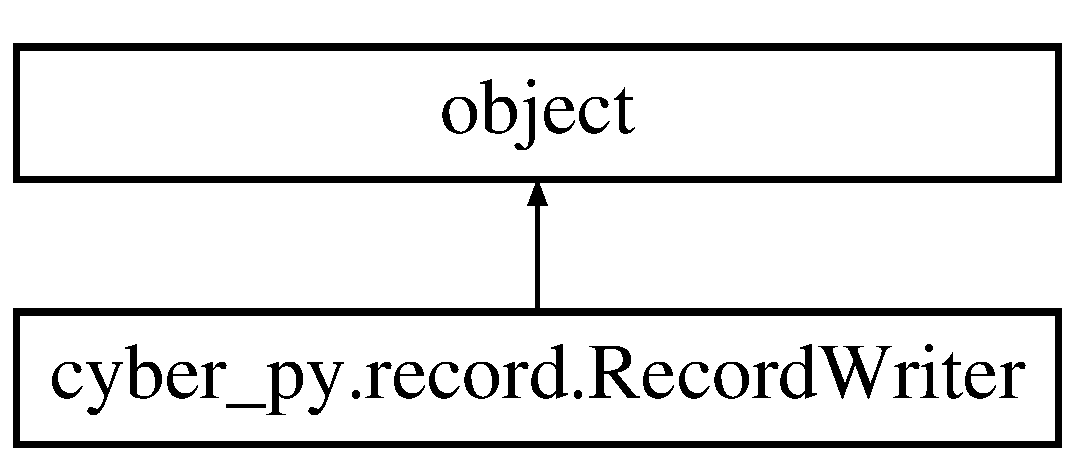
\includegraphics[height=2.000000cm]{classcyber__py_1_1record_1_1RecordWriter}
\end{center}
\end{figure}
\subsection*{Public Member Functions}
\begin{DoxyCompactItemize}
\item 
def \hyperlink{classcyber__py_1_1record_1_1RecordWriter_a14355714b318d04fb18339670b9bcb82}{\-\_\-\-\_\-init\-\_\-\-\_\-}
\item 
def \hyperlink{classcyber__py_1_1record_1_1RecordWriter_a03d3d431dedf40f2a865cc6caedc27b6}{\-\_\-\-\_\-del\-\_\-\-\_\-}
\item 
def \hyperlink{classcyber__py_1_1record_1_1RecordWriter_a1611664ff3f964ccd5821b0c5a2a8a85}{open}
\item 
def \hyperlink{classcyber__py_1_1record_1_1RecordWriter_a4876cf6805312cfd344e12e6474f72ae}{close}
\item 
def \hyperlink{classcyber__py_1_1record_1_1RecordWriter_a4cc5a7287e73a42fa9bf4bbca226e84f}{write\-\_\-channel}
\item 
def \hyperlink{classcyber__py_1_1record_1_1RecordWriter_a418eef3592ac895d1c57d127a3d979d2}{write\-\_\-message}
\item 
def \hyperlink{classcyber__py_1_1record_1_1RecordWriter_adf89b0a90fda34422edb0b5a36d7066a}{set\-\_\-size\-\_\-fileseg}
\item 
def \hyperlink{classcyber__py_1_1record_1_1RecordWriter_ae03b486b593d1818b06a9f9b7c45bdea}{set\-\_\-intervaltime\-\_\-fileseg}
\item 
def \hyperlink{classcyber__py_1_1record_1_1RecordWriter_a4e13eb41d36533dbaeedf7ec135576a9}{get\-\_\-messagenumber}
\item 
def \hyperlink{classcyber__py_1_1record_1_1RecordWriter_aaa2ebabc7fa95b2cf789f520e9b7a8a3}{get\-\_\-messagetype}
\item 
def \hyperlink{classcyber__py_1_1record_1_1RecordWriter_aae735e92351317e894f403ed542313ec}{get\-\_\-protodesc}
\end{DoxyCompactItemize}
\subsection*{Public Attributes}
\begin{DoxyCompactItemize}
\item 
\hyperlink{classcyber__py_1_1record_1_1RecordWriter_a398f5c011e8d8cc9dee542305ac22491}{record\-\_\-writer}
\end{DoxyCompactItemize}


\subsection{Detailed Description}
\begin{DoxyVerb}Class for cyber RecordWriter wrapper.
\end{DoxyVerb}
 

\subsection{Constructor \& Destructor Documentation}
\hypertarget{classcyber__py_1_1record_1_1RecordWriter_a14355714b318d04fb18339670b9bcb82}{\index{cyber\-\_\-py\-::record\-::\-Record\-Writer@{cyber\-\_\-py\-::record\-::\-Record\-Writer}!\-\_\-\-\_\-init\-\_\-\-\_\-@{\-\_\-\-\_\-init\-\_\-\-\_\-}}
\index{\-\_\-\-\_\-init\-\_\-\-\_\-@{\-\_\-\-\_\-init\-\_\-\-\_\-}!cyber_py::record::RecordWriter@{cyber\-\_\-py\-::record\-::\-Record\-Writer}}
\subsubsection[{\-\_\-\-\_\-init\-\_\-\-\_\-}]{\setlength{\rightskip}{0pt plus 5cm}def cyber\-\_\-py.\-record.\-Record\-Writer.\-\_\-\-\_\-init\-\_\-\-\_\- (
\begin{DoxyParamCaption}
\item[{}]{self, }
\item[{}]{file\-\_\-segmentation\-\_\-size\-\_\-kb = {\ttfamily 0}, }
\item[{}]{file\-\_\-segmentation\-\_\-interval\-\_\-sec = {\ttfamily 0}}
\end{DoxyParamCaption}
)}}\label{classcyber__py_1_1record_1_1RecordWriter_a14355714b318d04fb18339670b9bcb82}
\hypertarget{classcyber__py_1_1record_1_1RecordWriter_a03d3d431dedf40f2a865cc6caedc27b6}{\index{cyber\-\_\-py\-::record\-::\-Record\-Writer@{cyber\-\_\-py\-::record\-::\-Record\-Writer}!\-\_\-\-\_\-del\-\_\-\-\_\-@{\-\_\-\-\_\-del\-\_\-\-\_\-}}
\index{\-\_\-\-\_\-del\-\_\-\-\_\-@{\-\_\-\-\_\-del\-\_\-\-\_\-}!cyber_py::record::RecordWriter@{cyber\-\_\-py\-::record\-::\-Record\-Writer}}
\subsubsection[{\-\_\-\-\_\-del\-\_\-\-\_\-}]{\setlength{\rightskip}{0pt plus 5cm}def cyber\-\_\-py.\-record.\-Record\-Writer.\-\_\-\-\_\-del\-\_\-\-\_\- (
\begin{DoxyParamCaption}
\item[{}]{self}
\end{DoxyParamCaption}
)}}\label{classcyber__py_1_1record_1_1RecordWriter_a03d3d431dedf40f2a865cc6caedc27b6}


\subsection{Member Function Documentation}
\hypertarget{classcyber__py_1_1record_1_1RecordWriter_a4876cf6805312cfd344e12e6474f72ae}{\index{cyber\-\_\-py\-::record\-::\-Record\-Writer@{cyber\-\_\-py\-::record\-::\-Record\-Writer}!close@{close}}
\index{close@{close}!cyber_py::record::RecordWriter@{cyber\-\_\-py\-::record\-::\-Record\-Writer}}
\subsubsection[{close}]{\setlength{\rightskip}{0pt plus 5cm}def cyber\-\_\-py.\-record.\-Record\-Writer.\-close (
\begin{DoxyParamCaption}
\item[{}]{self}
\end{DoxyParamCaption}
)}}\label{classcyber__py_1_1record_1_1RecordWriter_a4876cf6805312cfd344e12e6474f72ae}
\begin{DoxyVerb}Close record file.
\end{DoxyVerb}
 \hypertarget{classcyber__py_1_1record_1_1RecordWriter_a4e13eb41d36533dbaeedf7ec135576a9}{\index{cyber\-\_\-py\-::record\-::\-Record\-Writer@{cyber\-\_\-py\-::record\-::\-Record\-Writer}!get\-\_\-messagenumber@{get\-\_\-messagenumber}}
\index{get\-\_\-messagenumber@{get\-\_\-messagenumber}!cyber_py::record::RecordWriter@{cyber\-\_\-py\-::record\-::\-Record\-Writer}}
\subsubsection[{get\-\_\-messagenumber}]{\setlength{\rightskip}{0pt plus 5cm}def cyber\-\_\-py.\-record.\-Record\-Writer.\-get\-\_\-messagenumber (
\begin{DoxyParamCaption}
\item[{}]{self, }
\item[{}]{channel\-\_\-name}
\end{DoxyParamCaption}
)}}\label{classcyber__py_1_1record_1_1RecordWriter_a4e13eb41d36533dbaeedf7ec135576a9}
\begin{DoxyVerb}Return message count.
\end{DoxyVerb}
 \hypertarget{classcyber__py_1_1record_1_1RecordWriter_aaa2ebabc7fa95b2cf789f520e9b7a8a3}{\index{cyber\-\_\-py\-::record\-::\-Record\-Writer@{cyber\-\_\-py\-::record\-::\-Record\-Writer}!get\-\_\-messagetype@{get\-\_\-messagetype}}
\index{get\-\_\-messagetype@{get\-\_\-messagetype}!cyber_py::record::RecordWriter@{cyber\-\_\-py\-::record\-::\-Record\-Writer}}
\subsubsection[{get\-\_\-messagetype}]{\setlength{\rightskip}{0pt plus 5cm}def cyber\-\_\-py.\-record.\-Record\-Writer.\-get\-\_\-messagetype (
\begin{DoxyParamCaption}
\item[{}]{self, }
\item[{}]{channel\-\_\-name}
\end{DoxyParamCaption}
)}}\label{classcyber__py_1_1record_1_1RecordWriter_aaa2ebabc7fa95b2cf789f520e9b7a8a3}
\begin{DoxyVerb}Return message type.
\end{DoxyVerb}
 \hypertarget{classcyber__py_1_1record_1_1RecordWriter_aae735e92351317e894f403ed542313ec}{\index{cyber\-\_\-py\-::record\-::\-Record\-Writer@{cyber\-\_\-py\-::record\-::\-Record\-Writer}!get\-\_\-protodesc@{get\-\_\-protodesc}}
\index{get\-\_\-protodesc@{get\-\_\-protodesc}!cyber_py::record::RecordWriter@{cyber\-\_\-py\-::record\-::\-Record\-Writer}}
\subsubsection[{get\-\_\-protodesc}]{\setlength{\rightskip}{0pt plus 5cm}def cyber\-\_\-py.\-record.\-Record\-Writer.\-get\-\_\-protodesc (
\begin{DoxyParamCaption}
\item[{}]{self, }
\item[{}]{channel\-\_\-name}
\end{DoxyParamCaption}
)}}\label{classcyber__py_1_1record_1_1RecordWriter_aae735e92351317e894f403ed542313ec}
\begin{DoxyVerb}Return message protodesc.
\end{DoxyVerb}
 \hypertarget{classcyber__py_1_1record_1_1RecordWriter_a1611664ff3f964ccd5821b0c5a2a8a85}{\index{cyber\-\_\-py\-::record\-::\-Record\-Writer@{cyber\-\_\-py\-::record\-::\-Record\-Writer}!open@{open}}
\index{open@{open}!cyber_py::record::RecordWriter@{cyber\-\_\-py\-::record\-::\-Record\-Writer}}
\subsubsection[{open}]{\setlength{\rightskip}{0pt plus 5cm}def cyber\-\_\-py.\-record.\-Record\-Writer.\-open (
\begin{DoxyParamCaption}
\item[{}]{self, }
\item[{}]{path}
\end{DoxyParamCaption}
)}}\label{classcyber__py_1_1record_1_1RecordWriter_a1611664ff3f964ccd5821b0c5a2a8a85}
\begin{DoxyVerb}Open record file for write.
\end{DoxyVerb}
 \hypertarget{classcyber__py_1_1record_1_1RecordWriter_ae03b486b593d1818b06a9f9b7c45bdea}{\index{cyber\-\_\-py\-::record\-::\-Record\-Writer@{cyber\-\_\-py\-::record\-::\-Record\-Writer}!set\-\_\-intervaltime\-\_\-fileseg@{set\-\_\-intervaltime\-\_\-fileseg}}
\index{set\-\_\-intervaltime\-\_\-fileseg@{set\-\_\-intervaltime\-\_\-fileseg}!cyber_py::record::RecordWriter@{cyber\-\_\-py\-::record\-::\-Record\-Writer}}
\subsubsection[{set\-\_\-intervaltime\-\_\-fileseg}]{\setlength{\rightskip}{0pt plus 5cm}def cyber\-\_\-py.\-record.\-Record\-Writer.\-set\-\_\-intervaltime\-\_\-fileseg (
\begin{DoxyParamCaption}
\item[{}]{self, }
\item[{}]{time\-\_\-sec}
\end{DoxyParamCaption}
)}}\label{classcyber__py_1_1record_1_1RecordWriter_ae03b486b593d1818b06a9f9b7c45bdea}
\begin{DoxyVerb}Return file interval time.
\end{DoxyVerb}
 \hypertarget{classcyber__py_1_1record_1_1RecordWriter_adf89b0a90fda34422edb0b5a36d7066a}{\index{cyber\-\_\-py\-::record\-::\-Record\-Writer@{cyber\-\_\-py\-::record\-::\-Record\-Writer}!set\-\_\-size\-\_\-fileseg@{set\-\_\-size\-\_\-fileseg}}
\index{set\-\_\-size\-\_\-fileseg@{set\-\_\-size\-\_\-fileseg}!cyber_py::record::RecordWriter@{cyber\-\_\-py\-::record\-::\-Record\-Writer}}
\subsubsection[{set\-\_\-size\-\_\-fileseg}]{\setlength{\rightskip}{0pt plus 5cm}def cyber\-\_\-py.\-record.\-Record\-Writer.\-set\-\_\-size\-\_\-fileseg (
\begin{DoxyParamCaption}
\item[{}]{self, }
\item[{}]{size\-\_\-kilobytes}
\end{DoxyParamCaption}
)}}\label{classcyber__py_1_1record_1_1RecordWriter_adf89b0a90fda34422edb0b5a36d7066a}
\begin{DoxyVerb}Return filesegment size.
\end{DoxyVerb}
 \hypertarget{classcyber__py_1_1record_1_1RecordWriter_a4cc5a7287e73a42fa9bf4bbca226e84f}{\index{cyber\-\_\-py\-::record\-::\-Record\-Writer@{cyber\-\_\-py\-::record\-::\-Record\-Writer}!write\-\_\-channel@{write\-\_\-channel}}
\index{write\-\_\-channel@{write\-\_\-channel}!cyber_py::record::RecordWriter@{cyber\-\_\-py\-::record\-::\-Record\-Writer}}
\subsubsection[{write\-\_\-channel}]{\setlength{\rightskip}{0pt plus 5cm}def cyber\-\_\-py.\-record.\-Record\-Writer.\-write\-\_\-channel (
\begin{DoxyParamCaption}
\item[{}]{self, }
\item[{}]{channel\-\_\-name, }
\item[{}]{type\-\_\-name, }
\item[{}]{proto\-\_\-desc}
\end{DoxyParamCaption}
)}}\label{classcyber__py_1_1record_1_1RecordWriter_a4cc5a7287e73a42fa9bf4bbca226e84f}
\begin{DoxyVerb}Writer channel by channelname,typename,protodesc
\end{DoxyVerb}
 \hypertarget{classcyber__py_1_1record_1_1RecordWriter_a418eef3592ac895d1c57d127a3d979d2}{\index{cyber\-\_\-py\-::record\-::\-Record\-Writer@{cyber\-\_\-py\-::record\-::\-Record\-Writer}!write\-\_\-message@{write\-\_\-message}}
\index{write\-\_\-message@{write\-\_\-message}!cyber_py::record::RecordWriter@{cyber\-\_\-py\-::record\-::\-Record\-Writer}}
\subsubsection[{write\-\_\-message}]{\setlength{\rightskip}{0pt plus 5cm}def cyber\-\_\-py.\-record.\-Record\-Writer.\-write\-\_\-message (
\begin{DoxyParamCaption}
\item[{}]{self, }
\item[{}]{channel\-\_\-name, }
\item[{}]{data, }
\item[{}]{time, }
\item[{}]{raw = {\ttfamily True}}
\end{DoxyParamCaption}
)}}\label{classcyber__py_1_1record_1_1RecordWriter_a418eef3592ac895d1c57d127a3d979d2}
\begin{DoxyVerb}Writer msg:channelname,rawmsg,writer time
\end{DoxyVerb}
 

\subsection{Member Data Documentation}
\hypertarget{classcyber__py_1_1record_1_1RecordWriter_a398f5c011e8d8cc9dee542305ac22491}{\index{cyber\-\_\-py\-::record\-::\-Record\-Writer@{cyber\-\_\-py\-::record\-::\-Record\-Writer}!record\-\_\-writer@{record\-\_\-writer}}
\index{record\-\_\-writer@{record\-\_\-writer}!cyber_py::record::RecordWriter@{cyber\-\_\-py\-::record\-::\-Record\-Writer}}
\subsubsection[{record\-\_\-writer}]{\setlength{\rightskip}{0pt plus 5cm}cyber\-\_\-py.\-record.\-Record\-Writer.\-record\-\_\-writer}}\label{classcyber__py_1_1record_1_1RecordWriter_a398f5c011e8d8cc9dee542305ac22491}


The documentation for this class was generated from the following file\-:\begin{DoxyCompactItemize}
\item 
python/cyber\-\_\-py/\hyperlink{record_8py}{record.\-py}\end{DoxyCompactItemize}

\hypertarget{classcyber__py_1_1cyber__time_1_1Time}{\section{cyber\-\_\-py.\-cyber\-\_\-time.\-Time Class Reference}
\label{classcyber__py_1_1cyber__time_1_1Time}\index{cyber\-\_\-py.\-cyber\-\_\-time.\-Time@{cyber\-\_\-py.\-cyber\-\_\-time.\-Time}}
}
Inheritance diagram for cyber\-\_\-py.\-cyber\-\_\-time.\-Time\-:\begin{figure}[H]
\begin{center}
\leavevmode
\includegraphics[height=2.000000cm]{classcyber__py_1_1cyber__time_1_1Time}
\end{center}
\end{figure}
\subsection*{Public Member Functions}
\begin{DoxyCompactItemize}
\item 
def \hyperlink{classcyber__py_1_1cyber__time_1_1Time_a10900825547906e8ce4d313cee2d94c6}{\-\_\-\-\_\-init\-\_\-\-\_\-}
\item 
def \hyperlink{classcyber__py_1_1cyber__time_1_1Time_aa41a2cfe16b372cab9a6e4e6ca18dac6}{\-\_\-\-\_\-del\-\_\-\-\_\-}
\item 
def \hyperlink{classcyber__py_1_1cyber__time_1_1Time_af88bec77617035d6054c9e892d5d62d0}{\-\_\-\-\_\-str\-\_\-\-\_\-}
\item 
def \hyperlink{classcyber__py_1_1cyber__time_1_1Time_aac227f91d90eb20b1704b8599f3d3af2}{iszero}
\item 
def \hyperlink{classcyber__py_1_1cyber__time_1_1Time_adcb2662bc1356197324062e53991f9ca}{to\-\_\-sec}
\item 
def \hyperlink{classcyber__py_1_1cyber__time_1_1Time_a60ed50a64dcf3b4effb8f7ebc45b4080}{to\-\_\-nsec}
\item 
def \hyperlink{classcyber__py_1_1cyber__time_1_1Time_a96b7103da36bd95764ce4f3d7aa8d0cd}{sleep\-\_\-until}
\item 
def \hyperlink{classcyber__py_1_1cyber__time_1_1Time_ae14102acffa6d707b4aef95d54d22bcd}{\-\_\-\-\_\-sub\-\_\-\-\_\-}
\item 
def \hyperlink{classcyber__py_1_1cyber__time_1_1Time_ad301fe1c623fcaa151ee95dded4049b3}{\-\_\-\-\_\-add\-\_\-\-\_\-}
\item 
def \hyperlink{classcyber__py_1_1cyber__time_1_1Time_a6f2903d2efc1c823e2ee19b9560f49a2}{\-\_\-\-\_\-radd\-\_\-\-\_\-}
\item 
def \hyperlink{classcyber__py_1_1cyber__time_1_1Time_a9f904f85ef0b1edddbe4002c5b276a81}{\-\_\-\-\_\-lt\-\_\-\-\_\-}
\item 
def \hyperlink{classcyber__py_1_1cyber__time_1_1Time_a1d33cc7f8de4afa4bd502249f60b402a}{\-\_\-\-\_\-gt\-\_\-\-\_\-}
\item 
def \hyperlink{classcyber__py_1_1cyber__time_1_1Time_a27ddc11ebbbd48aec91c41ac951e18ba}{\-\_\-\-\_\-le\-\_\-\-\_\-}
\item 
def \hyperlink{classcyber__py_1_1cyber__time_1_1Time_ad90eaaf4f702da516415fd153d0dbf15}{\-\_\-\-\_\-ge\-\_\-\-\_\-}
\item 
def \hyperlink{classcyber__py_1_1cyber__time_1_1Time_a034abca293a5e4a54e5f0190f66ff4d5}{\-\_\-\-\_\-eq\-\_\-\-\_\-}
\item 
def \hyperlink{classcyber__py_1_1cyber__time_1_1Time_a6e944bde380e451303866b3079a3f945}{\-\_\-\-\_\-ne\-\_\-\-\_\-}
\end{DoxyCompactItemize}
\subsection*{Static Public Member Functions}
\begin{DoxyCompactItemize}
\item 
def \hyperlink{classcyber__py_1_1cyber__time_1_1Time_a7730ee8a23b5e33b5090b554cea6cc05}{now}
\item 
def \hyperlink{classcyber__py_1_1cyber__time_1_1Time_a7f0d4009b78f4133c797fdb860af15e6}{mono\-\_\-time}
\end{DoxyCompactItemize}
\subsection*{Public Attributes}
\begin{DoxyCompactItemize}
\item 
\hyperlink{classcyber__py_1_1cyber__time_1_1Time_a2d81299f5e8afeea1e3a8807ffc9fb1f}{time}
\end{DoxyCompactItemize}


\subsection{Detailed Description}
\begin{DoxyVerb}Class for cyber time wrapper.
\end{DoxyVerb}
 

\subsection{Constructor \& Destructor Documentation}
\hypertarget{classcyber__py_1_1cyber__time_1_1Time_a10900825547906e8ce4d313cee2d94c6}{\index{cyber\-\_\-py\-::cyber\-\_\-time\-::\-Time@{cyber\-\_\-py\-::cyber\-\_\-time\-::\-Time}!\-\_\-\-\_\-init\-\_\-\-\_\-@{\-\_\-\-\_\-init\-\_\-\-\_\-}}
\index{\-\_\-\-\_\-init\-\_\-\-\_\-@{\-\_\-\-\_\-init\-\_\-\-\_\-}!cyber_py::cyber_time::Time@{cyber\-\_\-py\-::cyber\-\_\-time\-::\-Time}}
\subsubsection[{\-\_\-\-\_\-init\-\_\-\-\_\-}]{\setlength{\rightskip}{0pt plus 5cm}def cyber\-\_\-py.\-cyber\-\_\-time.\-Time.\-\_\-\-\_\-init\-\_\-\-\_\- (
\begin{DoxyParamCaption}
\item[{}]{self, }
\item[{}]{other}
\end{DoxyParamCaption}
)}}\label{classcyber__py_1_1cyber__time_1_1Time_a10900825547906e8ce4d313cee2d94c6}
\hypertarget{classcyber__py_1_1cyber__time_1_1Time_aa41a2cfe16b372cab9a6e4e6ca18dac6}{\index{cyber\-\_\-py\-::cyber\-\_\-time\-::\-Time@{cyber\-\_\-py\-::cyber\-\_\-time\-::\-Time}!\-\_\-\-\_\-del\-\_\-\-\_\-@{\-\_\-\-\_\-del\-\_\-\-\_\-}}
\index{\-\_\-\-\_\-del\-\_\-\-\_\-@{\-\_\-\-\_\-del\-\_\-\-\_\-}!cyber_py::cyber_time::Time@{cyber\-\_\-py\-::cyber\-\_\-time\-::\-Time}}
\subsubsection[{\-\_\-\-\_\-del\-\_\-\-\_\-}]{\setlength{\rightskip}{0pt plus 5cm}def cyber\-\_\-py.\-cyber\-\_\-time.\-Time.\-\_\-\-\_\-del\-\_\-\-\_\- (
\begin{DoxyParamCaption}
\item[{}]{self}
\end{DoxyParamCaption}
)}}\label{classcyber__py_1_1cyber__time_1_1Time_aa41a2cfe16b372cab9a6e4e6ca18dac6}


\subsection{Member Function Documentation}
\hypertarget{classcyber__py_1_1cyber__time_1_1Time_ad301fe1c623fcaa151ee95dded4049b3}{\index{cyber\-\_\-py\-::cyber\-\_\-time\-::\-Time@{cyber\-\_\-py\-::cyber\-\_\-time\-::\-Time}!\-\_\-\-\_\-add\-\_\-\-\_\-@{\-\_\-\-\_\-add\-\_\-\-\_\-}}
\index{\-\_\-\-\_\-add\-\_\-\-\_\-@{\-\_\-\-\_\-add\-\_\-\-\_\-}!cyber_py::cyber_time::Time@{cyber\-\_\-py\-::cyber\-\_\-time\-::\-Time}}
\subsubsection[{\-\_\-\-\_\-add\-\_\-\-\_\-}]{\setlength{\rightskip}{0pt plus 5cm}def cyber\-\_\-py.\-cyber\-\_\-time.\-Time.\-\_\-\-\_\-add\-\_\-\-\_\- (
\begin{DoxyParamCaption}
\item[{}]{self, }
\item[{}]{other}
\end{DoxyParamCaption}
)}}\label{classcyber__py_1_1cyber__time_1_1Time_ad301fe1c623fcaa151ee95dded4049b3}
\hypertarget{classcyber__py_1_1cyber__time_1_1Time_a034abca293a5e4a54e5f0190f66ff4d5}{\index{cyber\-\_\-py\-::cyber\-\_\-time\-::\-Time@{cyber\-\_\-py\-::cyber\-\_\-time\-::\-Time}!\-\_\-\-\_\-eq\-\_\-\-\_\-@{\-\_\-\-\_\-eq\-\_\-\-\_\-}}
\index{\-\_\-\-\_\-eq\-\_\-\-\_\-@{\-\_\-\-\_\-eq\-\_\-\-\_\-}!cyber_py::cyber_time::Time@{cyber\-\_\-py\-::cyber\-\_\-time\-::\-Time}}
\subsubsection[{\-\_\-\-\_\-eq\-\_\-\-\_\-}]{\setlength{\rightskip}{0pt plus 5cm}def cyber\-\_\-py.\-cyber\-\_\-time.\-Time.\-\_\-\-\_\-eq\-\_\-\-\_\- (
\begin{DoxyParamCaption}
\item[{}]{self, }
\item[{}]{other}
\end{DoxyParamCaption}
)}}\label{classcyber__py_1_1cyber__time_1_1Time_a034abca293a5e4a54e5f0190f66ff4d5}
\hypertarget{classcyber__py_1_1cyber__time_1_1Time_ad90eaaf4f702da516415fd153d0dbf15}{\index{cyber\-\_\-py\-::cyber\-\_\-time\-::\-Time@{cyber\-\_\-py\-::cyber\-\_\-time\-::\-Time}!\-\_\-\-\_\-ge\-\_\-\-\_\-@{\-\_\-\-\_\-ge\-\_\-\-\_\-}}
\index{\-\_\-\-\_\-ge\-\_\-\-\_\-@{\-\_\-\-\_\-ge\-\_\-\-\_\-}!cyber_py::cyber_time::Time@{cyber\-\_\-py\-::cyber\-\_\-time\-::\-Time}}
\subsubsection[{\-\_\-\-\_\-ge\-\_\-\-\_\-}]{\setlength{\rightskip}{0pt plus 5cm}def cyber\-\_\-py.\-cyber\-\_\-time.\-Time.\-\_\-\-\_\-ge\-\_\-\-\_\- (
\begin{DoxyParamCaption}
\item[{}]{self, }
\item[{}]{other}
\end{DoxyParamCaption}
)}}\label{classcyber__py_1_1cyber__time_1_1Time_ad90eaaf4f702da516415fd153d0dbf15}
\hypertarget{classcyber__py_1_1cyber__time_1_1Time_a1d33cc7f8de4afa4bd502249f60b402a}{\index{cyber\-\_\-py\-::cyber\-\_\-time\-::\-Time@{cyber\-\_\-py\-::cyber\-\_\-time\-::\-Time}!\-\_\-\-\_\-gt\-\_\-\-\_\-@{\-\_\-\-\_\-gt\-\_\-\-\_\-}}
\index{\-\_\-\-\_\-gt\-\_\-\-\_\-@{\-\_\-\-\_\-gt\-\_\-\-\_\-}!cyber_py::cyber_time::Time@{cyber\-\_\-py\-::cyber\-\_\-time\-::\-Time}}
\subsubsection[{\-\_\-\-\_\-gt\-\_\-\-\_\-}]{\setlength{\rightskip}{0pt plus 5cm}def cyber\-\_\-py.\-cyber\-\_\-time.\-Time.\-\_\-\-\_\-gt\-\_\-\-\_\- (
\begin{DoxyParamCaption}
\item[{}]{self, }
\item[{}]{other}
\end{DoxyParamCaption}
)}}\label{classcyber__py_1_1cyber__time_1_1Time_a1d33cc7f8de4afa4bd502249f60b402a}
\hypertarget{classcyber__py_1_1cyber__time_1_1Time_a27ddc11ebbbd48aec91c41ac951e18ba}{\index{cyber\-\_\-py\-::cyber\-\_\-time\-::\-Time@{cyber\-\_\-py\-::cyber\-\_\-time\-::\-Time}!\-\_\-\-\_\-le\-\_\-\-\_\-@{\-\_\-\-\_\-le\-\_\-\-\_\-}}
\index{\-\_\-\-\_\-le\-\_\-\-\_\-@{\-\_\-\-\_\-le\-\_\-\-\_\-}!cyber_py::cyber_time::Time@{cyber\-\_\-py\-::cyber\-\_\-time\-::\-Time}}
\subsubsection[{\-\_\-\-\_\-le\-\_\-\-\_\-}]{\setlength{\rightskip}{0pt plus 5cm}def cyber\-\_\-py.\-cyber\-\_\-time.\-Time.\-\_\-\-\_\-le\-\_\-\-\_\- (
\begin{DoxyParamCaption}
\item[{}]{self, }
\item[{}]{other}
\end{DoxyParamCaption}
)}}\label{classcyber__py_1_1cyber__time_1_1Time_a27ddc11ebbbd48aec91c41ac951e18ba}
\hypertarget{classcyber__py_1_1cyber__time_1_1Time_a9f904f85ef0b1edddbe4002c5b276a81}{\index{cyber\-\_\-py\-::cyber\-\_\-time\-::\-Time@{cyber\-\_\-py\-::cyber\-\_\-time\-::\-Time}!\-\_\-\-\_\-lt\-\_\-\-\_\-@{\-\_\-\-\_\-lt\-\_\-\-\_\-}}
\index{\-\_\-\-\_\-lt\-\_\-\-\_\-@{\-\_\-\-\_\-lt\-\_\-\-\_\-}!cyber_py::cyber_time::Time@{cyber\-\_\-py\-::cyber\-\_\-time\-::\-Time}}
\subsubsection[{\-\_\-\-\_\-lt\-\_\-\-\_\-}]{\setlength{\rightskip}{0pt plus 5cm}def cyber\-\_\-py.\-cyber\-\_\-time.\-Time.\-\_\-\-\_\-lt\-\_\-\-\_\- (
\begin{DoxyParamCaption}
\item[{}]{self, }
\item[{}]{other}
\end{DoxyParamCaption}
)}}\label{classcyber__py_1_1cyber__time_1_1Time_a9f904f85ef0b1edddbe4002c5b276a81}
\hypertarget{classcyber__py_1_1cyber__time_1_1Time_a6e944bde380e451303866b3079a3f945}{\index{cyber\-\_\-py\-::cyber\-\_\-time\-::\-Time@{cyber\-\_\-py\-::cyber\-\_\-time\-::\-Time}!\-\_\-\-\_\-ne\-\_\-\-\_\-@{\-\_\-\-\_\-ne\-\_\-\-\_\-}}
\index{\-\_\-\-\_\-ne\-\_\-\-\_\-@{\-\_\-\-\_\-ne\-\_\-\-\_\-}!cyber_py::cyber_time::Time@{cyber\-\_\-py\-::cyber\-\_\-time\-::\-Time}}
\subsubsection[{\-\_\-\-\_\-ne\-\_\-\-\_\-}]{\setlength{\rightskip}{0pt plus 5cm}def cyber\-\_\-py.\-cyber\-\_\-time.\-Time.\-\_\-\-\_\-ne\-\_\-\-\_\- (
\begin{DoxyParamCaption}
\item[{}]{self, }
\item[{}]{other}
\end{DoxyParamCaption}
)}}\label{classcyber__py_1_1cyber__time_1_1Time_a6e944bde380e451303866b3079a3f945}
\hypertarget{classcyber__py_1_1cyber__time_1_1Time_a6f2903d2efc1c823e2ee19b9560f49a2}{\index{cyber\-\_\-py\-::cyber\-\_\-time\-::\-Time@{cyber\-\_\-py\-::cyber\-\_\-time\-::\-Time}!\-\_\-\-\_\-radd\-\_\-\-\_\-@{\-\_\-\-\_\-radd\-\_\-\-\_\-}}
\index{\-\_\-\-\_\-radd\-\_\-\-\_\-@{\-\_\-\-\_\-radd\-\_\-\-\_\-}!cyber_py::cyber_time::Time@{cyber\-\_\-py\-::cyber\-\_\-time\-::\-Time}}
\subsubsection[{\-\_\-\-\_\-radd\-\_\-\-\_\-}]{\setlength{\rightskip}{0pt plus 5cm}def cyber\-\_\-py.\-cyber\-\_\-time.\-Time.\-\_\-\-\_\-radd\-\_\-\-\_\- (
\begin{DoxyParamCaption}
\item[{}]{self, }
\item[{}]{other}
\end{DoxyParamCaption}
)}}\label{classcyber__py_1_1cyber__time_1_1Time_a6f2903d2efc1c823e2ee19b9560f49a2}
\hypertarget{classcyber__py_1_1cyber__time_1_1Time_af88bec77617035d6054c9e892d5d62d0}{\index{cyber\-\_\-py\-::cyber\-\_\-time\-::\-Time@{cyber\-\_\-py\-::cyber\-\_\-time\-::\-Time}!\-\_\-\-\_\-str\-\_\-\-\_\-@{\-\_\-\-\_\-str\-\_\-\-\_\-}}
\index{\-\_\-\-\_\-str\-\_\-\-\_\-@{\-\_\-\-\_\-str\-\_\-\-\_\-}!cyber_py::cyber_time::Time@{cyber\-\_\-py\-::cyber\-\_\-time\-::\-Time}}
\subsubsection[{\-\_\-\-\_\-str\-\_\-\-\_\-}]{\setlength{\rightskip}{0pt plus 5cm}def cyber\-\_\-py.\-cyber\-\_\-time.\-Time.\-\_\-\-\_\-str\-\_\-\-\_\- (
\begin{DoxyParamCaption}
\item[{}]{self}
\end{DoxyParamCaption}
)}}\label{classcyber__py_1_1cyber__time_1_1Time_af88bec77617035d6054c9e892d5d62d0}
\hypertarget{classcyber__py_1_1cyber__time_1_1Time_ae14102acffa6d707b4aef95d54d22bcd}{\index{cyber\-\_\-py\-::cyber\-\_\-time\-::\-Time@{cyber\-\_\-py\-::cyber\-\_\-time\-::\-Time}!\-\_\-\-\_\-sub\-\_\-\-\_\-@{\-\_\-\-\_\-sub\-\_\-\-\_\-}}
\index{\-\_\-\-\_\-sub\-\_\-\-\_\-@{\-\_\-\-\_\-sub\-\_\-\-\_\-}!cyber_py::cyber_time::Time@{cyber\-\_\-py\-::cyber\-\_\-time\-::\-Time}}
\subsubsection[{\-\_\-\-\_\-sub\-\_\-\-\_\-}]{\setlength{\rightskip}{0pt plus 5cm}def cyber\-\_\-py.\-cyber\-\_\-time.\-Time.\-\_\-\-\_\-sub\-\_\-\-\_\- (
\begin{DoxyParamCaption}
\item[{}]{self, }
\item[{}]{other}
\end{DoxyParamCaption}
)}}\label{classcyber__py_1_1cyber__time_1_1Time_ae14102acffa6d707b4aef95d54d22bcd}
\hypertarget{classcyber__py_1_1cyber__time_1_1Time_aac227f91d90eb20b1704b8599f3d3af2}{\index{cyber\-\_\-py\-::cyber\-\_\-time\-::\-Time@{cyber\-\_\-py\-::cyber\-\_\-time\-::\-Time}!iszero@{iszero}}
\index{iszero@{iszero}!cyber_py::cyber_time::Time@{cyber\-\_\-py\-::cyber\-\_\-time\-::\-Time}}
\subsubsection[{iszero}]{\setlength{\rightskip}{0pt plus 5cm}def cyber\-\_\-py.\-cyber\-\_\-time.\-Time.\-iszero (
\begin{DoxyParamCaption}
\item[{}]{self}
\end{DoxyParamCaption}
)}}\label{classcyber__py_1_1cyber__time_1_1Time_aac227f91d90eb20b1704b8599f3d3af2}
\hypertarget{classcyber__py_1_1cyber__time_1_1Time_a7f0d4009b78f4133c797fdb860af15e6}{\index{cyber\-\_\-py\-::cyber\-\_\-time\-::\-Time@{cyber\-\_\-py\-::cyber\-\_\-time\-::\-Time}!mono\-\_\-time@{mono\-\_\-time}}
\index{mono\-\_\-time@{mono\-\_\-time}!cyber_py::cyber_time::Time@{cyber\-\_\-py\-::cyber\-\_\-time\-::\-Time}}
\subsubsection[{mono\-\_\-time}]{\setlength{\rightskip}{0pt plus 5cm}def cyber\-\_\-py.\-cyber\-\_\-time.\-Time.\-mono\-\_\-time (
\begin{DoxyParamCaption}
{}
\end{DoxyParamCaption}
)\hspace{0.3cm}{\ttfamily [static]}}}\label{classcyber__py_1_1cyber__time_1_1Time_a7f0d4009b78f4133c797fdb860af15e6}
\hypertarget{classcyber__py_1_1cyber__time_1_1Time_a7730ee8a23b5e33b5090b554cea6cc05}{\index{cyber\-\_\-py\-::cyber\-\_\-time\-::\-Time@{cyber\-\_\-py\-::cyber\-\_\-time\-::\-Time}!now@{now}}
\index{now@{now}!cyber_py::cyber_time::Time@{cyber\-\_\-py\-::cyber\-\_\-time\-::\-Time}}
\subsubsection[{now}]{\setlength{\rightskip}{0pt plus 5cm}def cyber\-\_\-py.\-cyber\-\_\-time.\-Time.\-now (
\begin{DoxyParamCaption}
{}
\end{DoxyParamCaption}
)\hspace{0.3cm}{\ttfamily [static]}}}\label{classcyber__py_1_1cyber__time_1_1Time_a7730ee8a23b5e33b5090b554cea6cc05}
\hypertarget{classcyber__py_1_1cyber__time_1_1Time_a96b7103da36bd95764ce4f3d7aa8d0cd}{\index{cyber\-\_\-py\-::cyber\-\_\-time\-::\-Time@{cyber\-\_\-py\-::cyber\-\_\-time\-::\-Time}!sleep\-\_\-until@{sleep\-\_\-until}}
\index{sleep\-\_\-until@{sleep\-\_\-until}!cyber_py::cyber_time::Time@{cyber\-\_\-py\-::cyber\-\_\-time\-::\-Time}}
\subsubsection[{sleep\-\_\-until}]{\setlength{\rightskip}{0pt plus 5cm}def cyber\-\_\-py.\-cyber\-\_\-time.\-Time.\-sleep\-\_\-until (
\begin{DoxyParamCaption}
\item[{}]{self, }
\item[{}]{nanoseconds}
\end{DoxyParamCaption}
)}}\label{classcyber__py_1_1cyber__time_1_1Time_a96b7103da36bd95764ce4f3d7aa8d0cd}
\hypertarget{classcyber__py_1_1cyber__time_1_1Time_a60ed50a64dcf3b4effb8f7ebc45b4080}{\index{cyber\-\_\-py\-::cyber\-\_\-time\-::\-Time@{cyber\-\_\-py\-::cyber\-\_\-time\-::\-Time}!to\-\_\-nsec@{to\-\_\-nsec}}
\index{to\-\_\-nsec@{to\-\_\-nsec}!cyber_py::cyber_time::Time@{cyber\-\_\-py\-::cyber\-\_\-time\-::\-Time}}
\subsubsection[{to\-\_\-nsec}]{\setlength{\rightskip}{0pt plus 5cm}def cyber\-\_\-py.\-cyber\-\_\-time.\-Time.\-to\-\_\-nsec (
\begin{DoxyParamCaption}
\item[{}]{self}
\end{DoxyParamCaption}
)}}\label{classcyber__py_1_1cyber__time_1_1Time_a60ed50a64dcf3b4effb8f7ebc45b4080}
\hypertarget{classcyber__py_1_1cyber__time_1_1Time_adcb2662bc1356197324062e53991f9ca}{\index{cyber\-\_\-py\-::cyber\-\_\-time\-::\-Time@{cyber\-\_\-py\-::cyber\-\_\-time\-::\-Time}!to\-\_\-sec@{to\-\_\-sec}}
\index{to\-\_\-sec@{to\-\_\-sec}!cyber_py::cyber_time::Time@{cyber\-\_\-py\-::cyber\-\_\-time\-::\-Time}}
\subsubsection[{to\-\_\-sec}]{\setlength{\rightskip}{0pt plus 5cm}def cyber\-\_\-py.\-cyber\-\_\-time.\-Time.\-to\-\_\-sec (
\begin{DoxyParamCaption}
\item[{}]{self}
\end{DoxyParamCaption}
)}}\label{classcyber__py_1_1cyber__time_1_1Time_adcb2662bc1356197324062e53991f9ca}


\subsection{Member Data Documentation}
\hypertarget{classcyber__py_1_1cyber__time_1_1Time_a2d81299f5e8afeea1e3a8807ffc9fb1f}{\index{cyber\-\_\-py\-::cyber\-\_\-time\-::\-Time@{cyber\-\_\-py\-::cyber\-\_\-time\-::\-Time}!time@{time}}
\index{time@{time}!cyber_py::cyber_time::Time@{cyber\-\_\-py\-::cyber\-\_\-time\-::\-Time}}
\subsubsection[{time}]{\setlength{\rightskip}{0pt plus 5cm}cyber\-\_\-py.\-cyber\-\_\-time.\-Time.\-time}}\label{classcyber__py_1_1cyber__time_1_1Time_a2d81299f5e8afeea1e3a8807ffc9fb1f}


The documentation for this class was generated from the following file\-:\begin{DoxyCompactItemize}
\item 
python/cyber\-\_\-py/\hyperlink{cyber__time_8py}{cyber\-\_\-time.\-py}\end{DoxyCompactItemize}

\hypertarget{classcyber__py_1_1cyber__timer_1_1Timer}{\section{cyber\-\_\-py.\-cyber\-\_\-timer.\-Timer Class Reference}
\label{classcyber__py_1_1cyber__timer_1_1Timer}\index{cyber\-\_\-py.\-cyber\-\_\-timer.\-Timer@{cyber\-\_\-py.\-cyber\-\_\-timer.\-Timer}}
}
Inheritance diagram for cyber\-\_\-py.\-cyber\-\_\-timer.\-Timer\-:\begin{figure}[H]
\begin{center}
\leavevmode
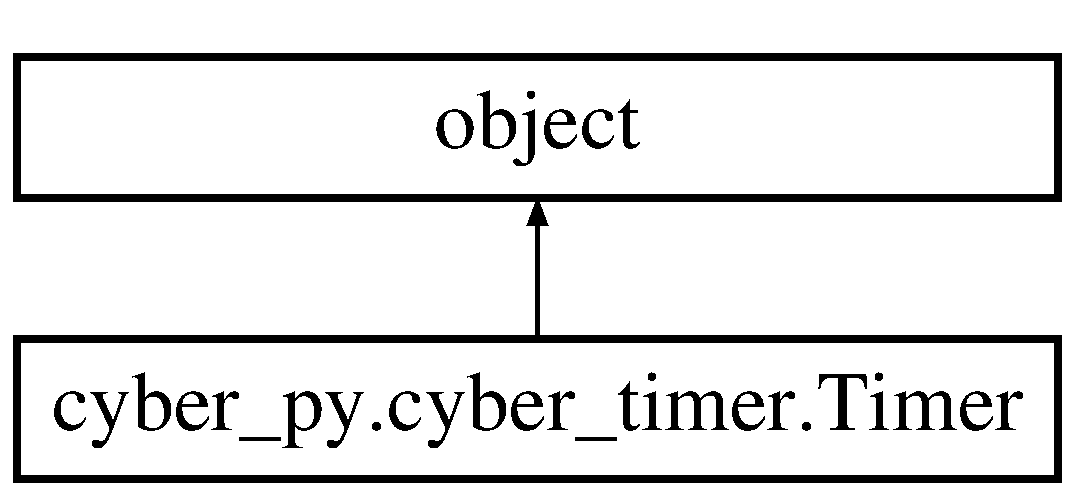
\includegraphics[height=2.000000cm]{classcyber__py_1_1cyber__timer_1_1Timer}
\end{center}
\end{figure}
\subsection*{Public Member Functions}
\begin{DoxyCompactItemize}
\item 
def \hyperlink{classcyber__py_1_1cyber__timer_1_1Timer_ad8c0267e9f4833c0adc21ad6f4769c77}{\-\_\-\-\_\-init\-\_\-\-\_\-}
\item 
def \hyperlink{classcyber__py_1_1cyber__timer_1_1Timer_a26e22ab1e79b079b021357c24c25d018}{\-\_\-\-\_\-del\-\_\-\-\_\-}
\item 
def \hyperlink{classcyber__py_1_1cyber__timer_1_1Timer_a68ec829dc37bfd878a96674964e80a14}{set\-\_\-option}
\item 
def \hyperlink{classcyber__py_1_1cyber__timer_1_1Timer_a8cb7bd524d4a9162ef3cbc664dc14c44}{start}
\item 
def \hyperlink{classcyber__py_1_1cyber__timer_1_1Timer_a7ae0beb18d25bf342224f51753c92939}{stop}
\end{DoxyCompactItemize}
\subsection*{Public Attributes}
\begin{DoxyCompactItemize}
\item 
\hyperlink{classcyber__py_1_1cyber__timer_1_1Timer_ab6eced17f6b54dbead937056a3e11def}{timer}
\item 
\hyperlink{classcyber__py_1_1cyber__timer_1_1Timer_a12707e11d95087467579b69228e0bfbe}{timer\-\_\-cb}
\item 
\hyperlink{classcyber__py_1_1cyber__timer_1_1Timer_a097dc3bac9a12163355d050d51dfb31b}{f\-\_\-ptr\-\_\-cb}
\end{DoxyCompactItemize}


\subsection{Detailed Description}
\begin{DoxyVerb}Class for cyber timer wrapper.
\end{DoxyVerb}
 

\subsection{Constructor \& Destructor Documentation}
\hypertarget{classcyber__py_1_1cyber__timer_1_1Timer_ad8c0267e9f4833c0adc21ad6f4769c77}{\index{cyber\-\_\-py\-::cyber\-\_\-timer\-::\-Timer@{cyber\-\_\-py\-::cyber\-\_\-timer\-::\-Timer}!\-\_\-\-\_\-init\-\_\-\-\_\-@{\-\_\-\-\_\-init\-\_\-\-\_\-}}
\index{\-\_\-\-\_\-init\-\_\-\-\_\-@{\-\_\-\-\_\-init\-\_\-\-\_\-}!cyber_py::cyber_timer::Timer@{cyber\-\_\-py\-::cyber\-\_\-timer\-::\-Timer}}
\subsubsection[{\-\_\-\-\_\-init\-\_\-\-\_\-}]{\setlength{\rightskip}{0pt plus 5cm}def cyber\-\_\-py.\-cyber\-\_\-timer.\-Timer.\-\_\-\-\_\-init\-\_\-\-\_\- (
\begin{DoxyParamCaption}
\item[{}]{self, }
\item[{}]{period = {\ttfamily None}, }
\item[{}]{callback = {\ttfamily None}, }
\item[{}]{oneshot = {\ttfamily None}}
\end{DoxyParamCaption}
)}}\label{classcyber__py_1_1cyber__timer_1_1Timer_ad8c0267e9f4833c0adc21ad6f4769c77}
\begin{DoxyVerb}period The period of the timer, unit is ms
callback The tasks that the timer needs to perform
oneshot 1: perform the callback only after the first timing cycle
0:perform the callback every timed period
\end{DoxyVerb}
 \hypertarget{classcyber__py_1_1cyber__timer_1_1Timer_a26e22ab1e79b079b021357c24c25d018}{\index{cyber\-\_\-py\-::cyber\-\_\-timer\-::\-Timer@{cyber\-\_\-py\-::cyber\-\_\-timer\-::\-Timer}!\-\_\-\-\_\-del\-\_\-\-\_\-@{\-\_\-\-\_\-del\-\_\-\-\_\-}}
\index{\-\_\-\-\_\-del\-\_\-\-\_\-@{\-\_\-\-\_\-del\-\_\-\-\_\-}!cyber_py::cyber_timer::Timer@{cyber\-\_\-py\-::cyber\-\_\-timer\-::\-Timer}}
\subsubsection[{\-\_\-\-\_\-del\-\_\-\-\_\-}]{\setlength{\rightskip}{0pt plus 5cm}def cyber\-\_\-py.\-cyber\-\_\-timer.\-Timer.\-\_\-\-\_\-del\-\_\-\-\_\- (
\begin{DoxyParamCaption}
\item[{}]{self}
\end{DoxyParamCaption}
)}}\label{classcyber__py_1_1cyber__timer_1_1Timer_a26e22ab1e79b079b021357c24c25d018}


\subsection{Member Function Documentation}
\hypertarget{classcyber__py_1_1cyber__timer_1_1Timer_a68ec829dc37bfd878a96674964e80a14}{\index{cyber\-\_\-py\-::cyber\-\_\-timer\-::\-Timer@{cyber\-\_\-py\-::cyber\-\_\-timer\-::\-Timer}!set\-\_\-option@{set\-\_\-option}}
\index{set\-\_\-option@{set\-\_\-option}!cyber_py::cyber_timer::Timer@{cyber\-\_\-py\-::cyber\-\_\-timer\-::\-Timer}}
\subsubsection[{set\-\_\-option}]{\setlength{\rightskip}{0pt plus 5cm}def cyber\-\_\-py.\-cyber\-\_\-timer.\-Timer.\-set\-\_\-option (
\begin{DoxyParamCaption}
\item[{}]{self, }
\item[{}]{period, }
\item[{}]{callback, }
\item[{}]{oneshot = {\ttfamily 0}}
\end{DoxyParamCaption}
)}}\label{classcyber__py_1_1cyber__timer_1_1Timer_a68ec829dc37bfd878a96674964e80a14}
\begin{DoxyVerb}period The period of the timer, unit is ms
callback The tasks that the timer needs to perform
oneshot 1: perform the callback only after the first timing cycle
0:perform the callback every timed period
\end{DoxyVerb}
 \hypertarget{classcyber__py_1_1cyber__timer_1_1Timer_a8cb7bd524d4a9162ef3cbc664dc14c44}{\index{cyber\-\_\-py\-::cyber\-\_\-timer\-::\-Timer@{cyber\-\_\-py\-::cyber\-\_\-timer\-::\-Timer}!start@{start}}
\index{start@{start}!cyber_py::cyber_timer::Timer@{cyber\-\_\-py\-::cyber\-\_\-timer\-::\-Timer}}
\subsubsection[{start}]{\setlength{\rightskip}{0pt plus 5cm}def cyber\-\_\-py.\-cyber\-\_\-timer.\-Timer.\-start (
\begin{DoxyParamCaption}
\item[{}]{self}
\end{DoxyParamCaption}
)}}\label{classcyber__py_1_1cyber__timer_1_1Timer_a8cb7bd524d4a9162ef3cbc664dc14c44}
\hypertarget{classcyber__py_1_1cyber__timer_1_1Timer_a7ae0beb18d25bf342224f51753c92939}{\index{cyber\-\_\-py\-::cyber\-\_\-timer\-::\-Timer@{cyber\-\_\-py\-::cyber\-\_\-timer\-::\-Timer}!stop@{stop}}
\index{stop@{stop}!cyber_py::cyber_timer::Timer@{cyber\-\_\-py\-::cyber\-\_\-timer\-::\-Timer}}
\subsubsection[{stop}]{\setlength{\rightskip}{0pt plus 5cm}def cyber\-\_\-py.\-cyber\-\_\-timer.\-Timer.\-stop (
\begin{DoxyParamCaption}
\item[{}]{self}
\end{DoxyParamCaption}
)}}\label{classcyber__py_1_1cyber__timer_1_1Timer_a7ae0beb18d25bf342224f51753c92939}


\subsection{Member Data Documentation}
\hypertarget{classcyber__py_1_1cyber__timer_1_1Timer_a097dc3bac9a12163355d050d51dfb31b}{\index{cyber\-\_\-py\-::cyber\-\_\-timer\-::\-Timer@{cyber\-\_\-py\-::cyber\-\_\-timer\-::\-Timer}!f\-\_\-ptr\-\_\-cb@{f\-\_\-ptr\-\_\-cb}}
\index{f\-\_\-ptr\-\_\-cb@{f\-\_\-ptr\-\_\-cb}!cyber_py::cyber_timer::Timer@{cyber\-\_\-py\-::cyber\-\_\-timer\-::\-Timer}}
\subsubsection[{f\-\_\-ptr\-\_\-cb}]{\setlength{\rightskip}{0pt plus 5cm}cyber\-\_\-py.\-cyber\-\_\-timer.\-Timer.\-f\-\_\-ptr\-\_\-cb}}\label{classcyber__py_1_1cyber__timer_1_1Timer_a097dc3bac9a12163355d050d51dfb31b}
\hypertarget{classcyber__py_1_1cyber__timer_1_1Timer_ab6eced17f6b54dbead937056a3e11def}{\index{cyber\-\_\-py\-::cyber\-\_\-timer\-::\-Timer@{cyber\-\_\-py\-::cyber\-\_\-timer\-::\-Timer}!timer@{timer}}
\index{timer@{timer}!cyber_py::cyber_timer::Timer@{cyber\-\_\-py\-::cyber\-\_\-timer\-::\-Timer}}
\subsubsection[{timer}]{\setlength{\rightskip}{0pt plus 5cm}cyber\-\_\-py.\-cyber\-\_\-timer.\-Timer.\-timer}}\label{classcyber__py_1_1cyber__timer_1_1Timer_ab6eced17f6b54dbead937056a3e11def}
\hypertarget{classcyber__py_1_1cyber__timer_1_1Timer_a12707e11d95087467579b69228e0bfbe}{\index{cyber\-\_\-py\-::cyber\-\_\-timer\-::\-Timer@{cyber\-\_\-py\-::cyber\-\_\-timer\-::\-Timer}!timer\-\_\-cb@{timer\-\_\-cb}}
\index{timer\-\_\-cb@{timer\-\_\-cb}!cyber_py::cyber_timer::Timer@{cyber\-\_\-py\-::cyber\-\_\-timer\-::\-Timer}}
\subsubsection[{timer\-\_\-cb}]{\setlength{\rightskip}{0pt plus 5cm}cyber\-\_\-py.\-cyber\-\_\-timer.\-Timer.\-timer\-\_\-cb}}\label{classcyber__py_1_1cyber__timer_1_1Timer_a12707e11d95087467579b69228e0bfbe}


The documentation for this class was generated from the following file\-:\begin{DoxyCompactItemize}
\item 
python/cyber\-\_\-py/\hyperlink{cyber__timer_8py}{cyber\-\_\-timer.\-py}\end{DoxyCompactItemize}

\hypertarget{classcyber__py_1_1topology__manager_1_1Topology__Manager}{\section{cyber\-\_\-py.\-topology\-\_\-manager.\-Topology\-\_\-\-Manager Class Reference}
\label{classcyber__py_1_1topology__manager_1_1Topology__Manager}\index{cyber\-\_\-py.\-topology\-\_\-manager.\-Topology\-\_\-\-Manager@{cyber\-\_\-py.\-topology\-\_\-manager.\-Topology\-\_\-\-Manager}}
}
Inheritance diagram for cyber\-\_\-py.\-topology\-\_\-manager.\-Topology\-\_\-\-Manager\-:\begin{figure}[H]
\begin{center}
\leavevmode
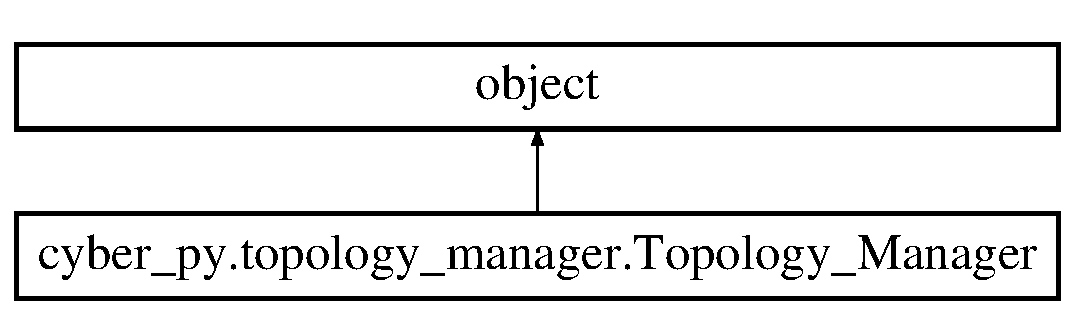
\includegraphics[height=2.000000cm]{classcyber__py_1_1topology__manager_1_1Topology__Manager}
\end{center}
\end{figure}
\subsection*{Public Member Functions}
\begin{DoxyCompactItemize}
\item 
def \hyperlink{classcyber__py_1_1topology__manager_1_1Topology__Manager_ab37f7a6c4197cf76f2a81da0ff0e83bc}{\-\_\-\-\_\-init\-\_\-\-\_\-}
\item 
def \hyperlink{classcyber__py_1_1topology__manager_1_1Topology__Manager_ae7b2631f17ffedd9d698609b23e49f8d}{has\-\_\-node}
\item 
def \hyperlink{classcyber__py_1_1topology__manager_1_1Topology__Manager_abcda716e82b70b85b068a08fbed9e853}{get\-\_\-node\-\_\-list}
\item 
def \hyperlink{classcyber__py_1_1topology__manager_1_1Topology__Manager_ab9299e6e3256eb8d6bace673c853bed5}{show\-\_\-node\-\_\-info}
\item 
def \hyperlink{classcyber__py_1_1topology__manager_1_1Topology__Manager_a6f39bf42627ff93b6a24372d721aa0ac}{get\-\_\-channel\-\_\-list}
\item 
def \hyperlink{classcyber__py_1_1topology__manager_1_1Topology__Manager_ac7200a996903f31bf38449997b6bac56}{get\-\_\-reader\-\_\-list}
\item 
def \hyperlink{classcyber__py_1_1topology__manager_1_1Topology__Manager_a9751fb4d8f196441da0552989c4dd47d}{get\-\_\-writer\-\_\-list}
\item 
def \hyperlink{classcyber__py_1_1topology__manager_1_1Topology__Manager_a6c1f7da4d2d899335824b25c70691348}{get\-\_\-node\-\_\-writes}
\item 
def \hyperlink{classcyber__py_1_1topology__manager_1_1Topology__Manager_a9d148e3c73f5323b18476974dd15f8da}{get\-\_\-node\-\_\-readers}
\item 
def \hyperlink{classcyber__py_1_1topology__manager_1_1Topology__Manager_a60bf7535b5c2634cf696e91e78f9ba21}{show\-\_\-channel\-\_\-info}
\end{DoxyCompactItemize}
\subsection*{Public Attributes}
\begin{DoxyCompactItemize}
\item 
\hyperlink{classcyber__py_1_1topology__manager_1_1Topology__Manager_a92f1604f7bb8557650abcde54dec6f56}{node\-\_\-manager}
\item 
\hyperlink{classcyber__py_1_1topology__manager_1_1Topology__Manager_ac2addb659e0d8b1081246cb69e1afed4}{channel\-\_\-manager}
\end{DoxyCompactItemize}


\subsection{Detailed Description}
\begin{DoxyVerb}Class for cyber Node wrapper.
\end{DoxyVerb}
 

\subsection{Constructor \& Destructor Documentation}
\hypertarget{classcyber__py_1_1topology__manager_1_1Topology__Manager_ab37f7a6c4197cf76f2a81da0ff0e83bc}{\index{cyber\-\_\-py\-::topology\-\_\-manager\-::\-Topology\-\_\-\-Manager@{cyber\-\_\-py\-::topology\-\_\-manager\-::\-Topology\-\_\-\-Manager}!\-\_\-\-\_\-init\-\_\-\-\_\-@{\-\_\-\-\_\-init\-\_\-\-\_\-}}
\index{\-\_\-\-\_\-init\-\_\-\-\_\-@{\-\_\-\-\_\-init\-\_\-\-\_\-}!cyber_py::topology_manager::Topology_Manager@{cyber\-\_\-py\-::topology\-\_\-manager\-::\-Topology\-\_\-\-Manager}}
\subsubsection[{\-\_\-\-\_\-init\-\_\-\-\_\-}]{\setlength{\rightskip}{0pt plus 5cm}def cyber\-\_\-py.\-topology\-\_\-manager.\-Topology\-\_\-\-Manager.\-\_\-\-\_\-init\-\_\-\-\_\- (
\begin{DoxyParamCaption}
\item[{}]{self}
\end{DoxyParamCaption}
)}}\label{classcyber__py_1_1topology__manager_1_1Topology__Manager_ab37f7a6c4197cf76f2a81da0ff0e83bc}
\begin{DoxyVerb}Init Topology Manager.
\end{DoxyVerb}
 

\subsection{Member Function Documentation}
\hypertarget{classcyber__py_1_1topology__manager_1_1Topology__Manager_a6f39bf42627ff93b6a24372d721aa0ac}{\index{cyber\-\_\-py\-::topology\-\_\-manager\-::\-Topology\-\_\-\-Manager@{cyber\-\_\-py\-::topology\-\_\-manager\-::\-Topology\-\_\-\-Manager}!get\-\_\-channel\-\_\-list@{get\-\_\-channel\-\_\-list}}
\index{get\-\_\-channel\-\_\-list@{get\-\_\-channel\-\_\-list}!cyber_py::topology_manager::Topology_Manager@{cyber\-\_\-py\-::topology\-\_\-manager\-::\-Topology\-\_\-\-Manager}}
\subsubsection[{get\-\_\-channel\-\_\-list}]{\setlength{\rightskip}{0pt plus 5cm}def cyber\-\_\-py.\-topology\-\_\-manager.\-Topology\-\_\-\-Manager.\-get\-\_\-channel\-\_\-list (
\begin{DoxyParamCaption}
\item[{}]{self}
\end{DoxyParamCaption}
)}}\label{classcyber__py_1_1topology__manager_1_1Topology__Manager_a6f39bf42627ff93b6a24372d721aa0ac}
\begin{DoxyVerb}Get Channel List.
\end{DoxyVerb}
 \hypertarget{classcyber__py_1_1topology__manager_1_1Topology__Manager_abcda716e82b70b85b068a08fbed9e853}{\index{cyber\-\_\-py\-::topology\-\_\-manager\-::\-Topology\-\_\-\-Manager@{cyber\-\_\-py\-::topology\-\_\-manager\-::\-Topology\-\_\-\-Manager}!get\-\_\-node\-\_\-list@{get\-\_\-node\-\_\-list}}
\index{get\-\_\-node\-\_\-list@{get\-\_\-node\-\_\-list}!cyber_py::topology_manager::Topology_Manager@{cyber\-\_\-py\-::topology\-\_\-manager\-::\-Topology\-\_\-\-Manager}}
\subsubsection[{get\-\_\-node\-\_\-list}]{\setlength{\rightskip}{0pt plus 5cm}def cyber\-\_\-py.\-topology\-\_\-manager.\-Topology\-\_\-\-Manager.\-get\-\_\-node\-\_\-list (
\begin{DoxyParamCaption}
\item[{}]{self}
\end{DoxyParamCaption}
)}}\label{classcyber__py_1_1topology__manager_1_1Topology__Manager_abcda716e82b70b85b068a08fbed9e853}
\begin{DoxyVerb}Get Node List.
\end{DoxyVerb}
 \hypertarget{classcyber__py_1_1topology__manager_1_1Topology__Manager_a9d148e3c73f5323b18476974dd15f8da}{\index{cyber\-\_\-py\-::topology\-\_\-manager\-::\-Topology\-\_\-\-Manager@{cyber\-\_\-py\-::topology\-\_\-manager\-::\-Topology\-\_\-\-Manager}!get\-\_\-node\-\_\-readers@{get\-\_\-node\-\_\-readers}}
\index{get\-\_\-node\-\_\-readers@{get\-\_\-node\-\_\-readers}!cyber_py::topology_manager::Topology_Manager@{cyber\-\_\-py\-::topology\-\_\-manager\-::\-Topology\-\_\-\-Manager}}
\subsubsection[{get\-\_\-node\-\_\-readers}]{\setlength{\rightskip}{0pt plus 5cm}def cyber\-\_\-py.\-topology\-\_\-manager.\-Topology\-\_\-\-Manager.\-get\-\_\-node\-\_\-readers (
\begin{DoxyParamCaption}
\item[{}]{self, }
\item[{}]{node\-\_\-name}
\end{DoxyParamCaption}
)}}\label{classcyber__py_1_1topology__manager_1_1Topology__Manager_a9d148e3c73f5323b18476974dd15f8da}
\begin{DoxyVerb}Get Node Readers.
\end{DoxyVerb}
 \hypertarget{classcyber__py_1_1topology__manager_1_1Topology__Manager_a6c1f7da4d2d899335824b25c70691348}{\index{cyber\-\_\-py\-::topology\-\_\-manager\-::\-Topology\-\_\-\-Manager@{cyber\-\_\-py\-::topology\-\_\-manager\-::\-Topology\-\_\-\-Manager}!get\-\_\-node\-\_\-writes@{get\-\_\-node\-\_\-writes}}
\index{get\-\_\-node\-\_\-writes@{get\-\_\-node\-\_\-writes}!cyber_py::topology_manager::Topology_Manager@{cyber\-\_\-py\-::topology\-\_\-manager\-::\-Topology\-\_\-\-Manager}}
\subsubsection[{get\-\_\-node\-\_\-writes}]{\setlength{\rightskip}{0pt plus 5cm}def cyber\-\_\-py.\-topology\-\_\-manager.\-Topology\-\_\-\-Manager.\-get\-\_\-node\-\_\-writes (
\begin{DoxyParamCaption}
\item[{}]{self, }
\item[{}]{node\-\_\-name}
\end{DoxyParamCaption}
)}}\label{classcyber__py_1_1topology__manager_1_1Topology__Manager_a6c1f7da4d2d899335824b25c70691348}
\begin{DoxyVerb}Get Node Writes.
\end{DoxyVerb}
 \hypertarget{classcyber__py_1_1topology__manager_1_1Topology__Manager_ac7200a996903f31bf38449997b6bac56}{\index{cyber\-\_\-py\-::topology\-\_\-manager\-::\-Topology\-\_\-\-Manager@{cyber\-\_\-py\-::topology\-\_\-manager\-::\-Topology\-\_\-\-Manager}!get\-\_\-reader\-\_\-list@{get\-\_\-reader\-\_\-list}}
\index{get\-\_\-reader\-\_\-list@{get\-\_\-reader\-\_\-list}!cyber_py::topology_manager::Topology_Manager@{cyber\-\_\-py\-::topology\-\_\-manager\-::\-Topology\-\_\-\-Manager}}
\subsubsection[{get\-\_\-reader\-\_\-list}]{\setlength{\rightskip}{0pt plus 5cm}def cyber\-\_\-py.\-topology\-\_\-manager.\-Topology\-\_\-\-Manager.\-get\-\_\-reader\-\_\-list (
\begin{DoxyParamCaption}
\item[{}]{self}
\end{DoxyParamCaption}
)}}\label{classcyber__py_1_1topology__manager_1_1Topology__Manager_ac7200a996903f31bf38449997b6bac56}
\begin{DoxyVerb}Get Reader List.
\end{DoxyVerb}
 \hypertarget{classcyber__py_1_1topology__manager_1_1Topology__Manager_a9751fb4d8f196441da0552989c4dd47d}{\index{cyber\-\_\-py\-::topology\-\_\-manager\-::\-Topology\-\_\-\-Manager@{cyber\-\_\-py\-::topology\-\_\-manager\-::\-Topology\-\_\-\-Manager}!get\-\_\-writer\-\_\-list@{get\-\_\-writer\-\_\-list}}
\index{get\-\_\-writer\-\_\-list@{get\-\_\-writer\-\_\-list}!cyber_py::topology_manager::Topology_Manager@{cyber\-\_\-py\-::topology\-\_\-manager\-::\-Topology\-\_\-\-Manager}}
\subsubsection[{get\-\_\-writer\-\_\-list}]{\setlength{\rightskip}{0pt plus 5cm}def cyber\-\_\-py.\-topology\-\_\-manager.\-Topology\-\_\-\-Manager.\-get\-\_\-writer\-\_\-list (
\begin{DoxyParamCaption}
\item[{}]{self}
\end{DoxyParamCaption}
)}}\label{classcyber__py_1_1topology__manager_1_1Topology__Manager_a9751fb4d8f196441da0552989c4dd47d}
\begin{DoxyVerb}Get Writer List.
\end{DoxyVerb}
 \hypertarget{classcyber__py_1_1topology__manager_1_1Topology__Manager_ae7b2631f17ffedd9d698609b23e49f8d}{\index{cyber\-\_\-py\-::topology\-\_\-manager\-::\-Topology\-\_\-\-Manager@{cyber\-\_\-py\-::topology\-\_\-manager\-::\-Topology\-\_\-\-Manager}!has\-\_\-node@{has\-\_\-node}}
\index{has\-\_\-node@{has\-\_\-node}!cyber_py::topology_manager::Topology_Manager@{cyber\-\_\-py\-::topology\-\_\-manager\-::\-Topology\-\_\-\-Manager}}
\subsubsection[{has\-\_\-node}]{\setlength{\rightskip}{0pt plus 5cm}def cyber\-\_\-py.\-topology\-\_\-manager.\-Topology\-\_\-\-Manager.\-has\-\_\-node (
\begin{DoxyParamCaption}
\item[{}]{self, }
\item[{}]{node\-\_\-name}
\end{DoxyParamCaption}
)}}\label{classcyber__py_1_1topology__manager_1_1Topology__Manager_ae7b2631f17ffedd9d698609b23e49f8d}
\begin{DoxyVerb}check Has Specific Node.
\end{DoxyVerb}
 \hypertarget{classcyber__py_1_1topology__manager_1_1Topology__Manager_a60bf7535b5c2634cf696e91e78f9ba21}{\index{cyber\-\_\-py\-::topology\-\_\-manager\-::\-Topology\-\_\-\-Manager@{cyber\-\_\-py\-::topology\-\_\-manager\-::\-Topology\-\_\-\-Manager}!show\-\_\-channel\-\_\-info@{show\-\_\-channel\-\_\-info}}
\index{show\-\_\-channel\-\_\-info@{show\-\_\-channel\-\_\-info}!cyber_py::topology_manager::Topology_Manager@{cyber\-\_\-py\-::topology\-\_\-manager\-::\-Topology\-\_\-\-Manager}}
\subsubsection[{show\-\_\-channel\-\_\-info}]{\setlength{\rightskip}{0pt plus 5cm}def cyber\-\_\-py.\-topology\-\_\-manager.\-Topology\-\_\-\-Manager.\-show\-\_\-channel\-\_\-info (
\begin{DoxyParamCaption}
\item[{}]{self, }
\item[{}]{channel\-\_\-name}
\end{DoxyParamCaption}
)}}\label{classcyber__py_1_1topology__manager_1_1Topology__Manager_a60bf7535b5c2634cf696e91e78f9ba21}
\begin{DoxyVerb}Show Channel Info.
\end{DoxyVerb}
 \hypertarget{classcyber__py_1_1topology__manager_1_1Topology__Manager_ab9299e6e3256eb8d6bace673c853bed5}{\index{cyber\-\_\-py\-::topology\-\_\-manager\-::\-Topology\-\_\-\-Manager@{cyber\-\_\-py\-::topology\-\_\-manager\-::\-Topology\-\_\-\-Manager}!show\-\_\-node\-\_\-info@{show\-\_\-node\-\_\-info}}
\index{show\-\_\-node\-\_\-info@{show\-\_\-node\-\_\-info}!cyber_py::topology_manager::Topology_Manager@{cyber\-\_\-py\-::topology\-\_\-manager\-::\-Topology\-\_\-\-Manager}}
\subsubsection[{show\-\_\-node\-\_\-info}]{\setlength{\rightskip}{0pt plus 5cm}def cyber\-\_\-py.\-topology\-\_\-manager.\-Topology\-\_\-\-Manager.\-show\-\_\-node\-\_\-info (
\begin{DoxyParamCaption}
\item[{}]{self, }
\item[{}]{node\-\_\-name}
\end{DoxyParamCaption}
)}}\label{classcyber__py_1_1topology__manager_1_1Topology__Manager_ab9299e6e3256eb8d6bace673c853bed5}
\begin{DoxyVerb}Show Node Info.
\end{DoxyVerb}
 

\subsection{Member Data Documentation}
\hypertarget{classcyber__py_1_1topology__manager_1_1Topology__Manager_ac2addb659e0d8b1081246cb69e1afed4}{\index{cyber\-\_\-py\-::topology\-\_\-manager\-::\-Topology\-\_\-\-Manager@{cyber\-\_\-py\-::topology\-\_\-manager\-::\-Topology\-\_\-\-Manager}!channel\-\_\-manager@{channel\-\_\-manager}}
\index{channel\-\_\-manager@{channel\-\_\-manager}!cyber_py::topology_manager::Topology_Manager@{cyber\-\_\-py\-::topology\-\_\-manager\-::\-Topology\-\_\-\-Manager}}
\subsubsection[{channel\-\_\-manager}]{\setlength{\rightskip}{0pt plus 5cm}cyber\-\_\-py.\-topology\-\_\-manager.\-Topology\-\_\-\-Manager.\-channel\-\_\-manager}}\label{classcyber__py_1_1topology__manager_1_1Topology__Manager_ac2addb659e0d8b1081246cb69e1afed4}
\hypertarget{classcyber__py_1_1topology__manager_1_1Topology__Manager_a92f1604f7bb8557650abcde54dec6f56}{\index{cyber\-\_\-py\-::topology\-\_\-manager\-::\-Topology\-\_\-\-Manager@{cyber\-\_\-py\-::topology\-\_\-manager\-::\-Topology\-\_\-\-Manager}!node\-\_\-manager@{node\-\_\-manager}}
\index{node\-\_\-manager@{node\-\_\-manager}!cyber_py::topology_manager::Topology_Manager@{cyber\-\_\-py\-::topology\-\_\-manager\-::\-Topology\-\_\-\-Manager}}
\subsubsection[{node\-\_\-manager}]{\setlength{\rightskip}{0pt plus 5cm}cyber\-\_\-py.\-topology\-\_\-manager.\-Topology\-\_\-\-Manager.\-node\-\_\-manager}}\label{classcyber__py_1_1topology__manager_1_1Topology__Manager_a92f1604f7bb8557650abcde54dec6f56}


The documentation for this class was generated from the following file\-:\begin{DoxyCompactItemize}
\item 
python/cyber\-\_\-py/\hyperlink{topology__manager_8py}{topology\-\_\-manager.\-py}\end{DoxyCompactItemize}

\hypertarget{classcyber__py_1_1cyber_1_1Writer}{\section{cyber\-\_\-py.\-cyber.\-Writer Class Reference}
\label{classcyber__py_1_1cyber_1_1Writer}\index{cyber\-\_\-py.\-cyber.\-Writer@{cyber\-\_\-py.\-cyber.\-Writer}}
}
Inheritance diagram for cyber\-\_\-py.\-cyber.\-Writer\-:\begin{figure}[H]
\begin{center}
\leavevmode
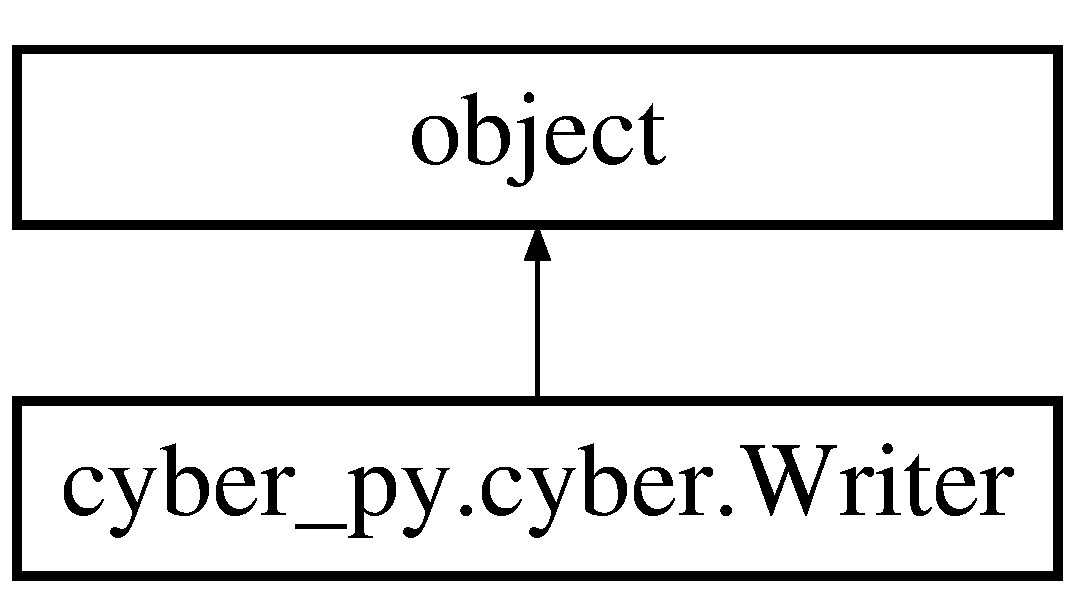
\includegraphics[height=2.000000cm]{classcyber__py_1_1cyber_1_1Writer}
\end{center}
\end{figure}
\subsection*{Public Member Functions}
\begin{DoxyCompactItemize}
\item 
def \hyperlink{classcyber__py_1_1cyber_1_1Writer_a1c8622d8858c2703dedd6527fc1c654b}{\-\_\-\-\_\-init\-\_\-\-\_\-}
\item 
def \hyperlink{classcyber__py_1_1cyber_1_1Writer_a5ef5ce319cfcb085266ffa8e6cb6cae2}{write}
\end{DoxyCompactItemize}
\subsection*{Public Attributes}
\begin{DoxyCompactItemize}
\item 
\hyperlink{classcyber__py_1_1cyber_1_1Writer_aae9aa5c2f9390d4ab157294a29c7d2a2}{name}
\item 
\hyperlink{classcyber__py_1_1cyber_1_1Writer_a560cf803725f9c259059956211418582}{writer}
\item 
\hyperlink{classcyber__py_1_1cyber_1_1Writer_a9ad78a9c6ec32e9cc9f56cff9c6be6ad}{data\-\_\-type}
\end{DoxyCompactItemize}


\subsection{Detailed Description}
\begin{DoxyVerb}Class for cyber writer wrapper.
\end{DoxyVerb}
 

\subsection{Constructor \& Destructor Documentation}
\hypertarget{classcyber__py_1_1cyber_1_1Writer_a1c8622d8858c2703dedd6527fc1c654b}{\index{cyber\-\_\-py\-::cyber\-::\-Writer@{cyber\-\_\-py\-::cyber\-::\-Writer}!\-\_\-\-\_\-init\-\_\-\-\_\-@{\-\_\-\-\_\-init\-\_\-\-\_\-}}
\index{\-\_\-\-\_\-init\-\_\-\-\_\-@{\-\_\-\-\_\-init\-\_\-\-\_\-}!cyber_py::cyber::Writer@{cyber\-\_\-py\-::cyber\-::\-Writer}}
\subsubsection[{\-\_\-\-\_\-init\-\_\-\-\_\-}]{\setlength{\rightskip}{0pt plus 5cm}def cyber\-\_\-py.\-cyber.\-Writer.\-\_\-\-\_\-init\-\_\-\-\_\- (
\begin{DoxyParamCaption}
\item[{}]{self, }
\item[{}]{name, }
\item[{}]{writer, }
\item[{}]{data\-\_\-type}
\end{DoxyParamCaption}
)}}\label{classcyber__py_1_1cyber_1_1Writer_a1c8622d8858c2703dedd6527fc1c654b}


\subsection{Member Function Documentation}
\hypertarget{classcyber__py_1_1cyber_1_1Writer_a5ef5ce319cfcb085266ffa8e6cb6cae2}{\index{cyber\-\_\-py\-::cyber\-::\-Writer@{cyber\-\_\-py\-::cyber\-::\-Writer}!write@{write}}
\index{write@{write}!cyber_py::cyber::Writer@{cyber\-\_\-py\-::cyber\-::\-Writer}}
\subsubsection[{write}]{\setlength{\rightskip}{0pt plus 5cm}def cyber\-\_\-py.\-cyber.\-Writer.\-write (
\begin{DoxyParamCaption}
\item[{}]{self, }
\item[{}]{data}
\end{DoxyParamCaption}
)}}\label{classcyber__py_1_1cyber_1_1Writer_a5ef5ce319cfcb085266ffa8e6cb6cae2}
\begin{DoxyVerb}writer msg string
\end{DoxyVerb}
 

\subsection{Member Data Documentation}
\hypertarget{classcyber__py_1_1cyber_1_1Writer_a9ad78a9c6ec32e9cc9f56cff9c6be6ad}{\index{cyber\-\_\-py\-::cyber\-::\-Writer@{cyber\-\_\-py\-::cyber\-::\-Writer}!data\-\_\-type@{data\-\_\-type}}
\index{data\-\_\-type@{data\-\_\-type}!cyber_py::cyber::Writer@{cyber\-\_\-py\-::cyber\-::\-Writer}}
\subsubsection[{data\-\_\-type}]{\setlength{\rightskip}{0pt plus 5cm}cyber\-\_\-py.\-cyber.\-Writer.\-data\-\_\-type}}\label{classcyber__py_1_1cyber_1_1Writer_a9ad78a9c6ec32e9cc9f56cff9c6be6ad}
\hypertarget{classcyber__py_1_1cyber_1_1Writer_aae9aa5c2f9390d4ab157294a29c7d2a2}{\index{cyber\-\_\-py\-::cyber\-::\-Writer@{cyber\-\_\-py\-::cyber\-::\-Writer}!name@{name}}
\index{name@{name}!cyber_py::cyber::Writer@{cyber\-\_\-py\-::cyber\-::\-Writer}}
\subsubsection[{name}]{\setlength{\rightskip}{0pt plus 5cm}cyber\-\_\-py.\-cyber.\-Writer.\-name}}\label{classcyber__py_1_1cyber_1_1Writer_aae9aa5c2f9390d4ab157294a29c7d2a2}
\hypertarget{classcyber__py_1_1cyber_1_1Writer_a560cf803725f9c259059956211418582}{\index{cyber\-\_\-py\-::cyber\-::\-Writer@{cyber\-\_\-py\-::cyber\-::\-Writer}!writer@{writer}}
\index{writer@{writer}!cyber_py::cyber::Writer@{cyber\-\_\-py\-::cyber\-::\-Writer}}
\subsubsection[{writer}]{\setlength{\rightskip}{0pt plus 5cm}cyber\-\_\-py.\-cyber.\-Writer.\-writer}}\label{classcyber__py_1_1cyber_1_1Writer_a560cf803725f9c259059956211418582}


The documentation for this class was generated from the following file\-:\begin{DoxyCompactItemize}
\item 
python/cyber\-\_\-py/\hyperlink{cyber_8py}{cyber.\-py}\end{DoxyCompactItemize}

\chapter{File Documentation}
\hypertarget{cyber_8py}{\section{python/cyber\-\_\-py/cyber.py File Reference}
\label{cyber_8py}\index{python/cyber\-\_\-py/cyber.\-py@{python/cyber\-\_\-py/cyber.\-py}}
}
\subsection*{Classes}
\begin{DoxyCompactItemize}
\item 
class \hyperlink{classcyber__py_1_1cyber_1_1Writer}{cyber\-\_\-py.\-cyber.\-Writer}
\item 
class \hyperlink{classcyber__py_1_1cyber_1_1Reader}{cyber\-\_\-py.\-cyber.\-Reader}
\item 
class \hyperlink{classcyber__py_1_1cyber_1_1Client}{cyber\-\_\-py.\-cyber.\-Client}
\item 
class \hyperlink{classcyber__py_1_1cyber_1_1Node}{cyber\-\_\-py.\-cyber.\-Node}
\end{DoxyCompactItemize}
\subsection*{Namespaces}
\begin{DoxyCompactItemize}
\item 
\hyperlink{namespacecyber__py_1_1cyber}{cyber\-\_\-py.\-cyber}
\end{DoxyCompactItemize}
\subsection*{Functions}
\begin{DoxyCompactItemize}
\item 
def \hyperlink{namespacecyber__py_1_1cyber_ac5dda5ce1579255672ccd20e200eef6e}{cyber\-\_\-py.\-cyber.\-init}
\item 
def \hyperlink{namespacecyber__py_1_1cyber_aacd6b88be138f317081a3270aac80eb4}{cyber\-\_\-py.\-cyber.\-ok}
\item 
def \hyperlink{namespacecyber__py_1_1cyber_a7977093d48defe12009683277367d2f6}{cyber\-\_\-py.\-cyber.\-shutdown}
\item 
def \hyperlink{namespacecyber__py_1_1cyber_ab17bb5a61b146ffd5050f4bc28370bea}{cyber\-\_\-py.\-cyber.\-is\-\_\-shutdown}
\item 
def \hyperlink{namespacecyber__py_1_1cyber_a017bbe6726341a06f0ae2b9cea0918c3}{cyber\-\_\-py.\-cyber.\-waitforshutdown}
\end{DoxyCompactItemize}
\subsection*{Variables}
\begin{DoxyCompactItemize}
\item 
tuple \hyperlink{namespacecyber__py_1_1cyber_ae9dc2f6ce4ac3380ed0e7fef03ff278f}{cyber\-\_\-py.\-cyber.\-P\-Y\-\_\-\-C\-A\-L\-L\-B\-A\-C\-K\-\_\-\-T\-Y\-P\-E} = ctypes.\-C\-F\-U\-N\-C\-T\-Y\-P\-E(ctypes.\-c\-\_\-int, ctypes.\-c\-\_\-char\-\_\-p)
\item 
tuple \hyperlink{namespacecyber__py_1_1cyber_a1e4152c96fe4765932b8125fe1f603fa}{cyber\-\_\-py.\-cyber.\-P\-Y\-\_\-\-C\-A\-L\-L\-B\-A\-C\-K\-\_\-\-T\-Y\-P\-E\-\_\-\-T} = ctypes.\-C\-F\-U\-N\-C\-T\-Y\-P\-E(ctypes.\-c\-\_\-int, ctypes.\-c\-\_\-char\-\_\-p)
\item 
list \hyperlink{namespacecyber__py_1_1cyber_a512e2d9892caf9598327c8238f9099a7}{cyber\-\_\-py.\-cyber.\-C\-Y\-B\-E\-R\-\_\-\-P\-A\-T\-H} = os.\-environ\mbox{[}'C\-Y\-B\-E\-R\-\_\-\-P\-A\-T\-H'\mbox{]}
\item 
tuple \hyperlink{namespacecyber__py_1_1cyber_a9ad5920bb49c68afc605b57816eda7d8}{cyber\-\_\-py.\-cyber.\-C\-Y\-B\-E\-R\-\_\-\-D\-I\-R} = os.\-path.\-split(C\-Y\-B\-E\-R\-\_\-\-P\-A\-T\-H)
\item 
tuple \hyperlink{namespacecyber__py_1_1cyber_a21aad6bb1a9e36085a1080ee9ef1de44}{cyber\-\_\-py.\-cyber.\-\_\-\-C\-Y\-B\-E\-R\-\_\-\-I\-N\-I\-T} = importlib.\-import\-\_\-module('\-\_\-cyber\-\_\-init')
\item 
tuple \hyperlink{namespacecyber__py_1_1cyber_aebfa8caeeb1ae0bf47733f9c2a184f93}{cyber\-\_\-py.\-cyber.\-\_\-\-C\-Y\-B\-E\-R\-\_\-\-N\-O\-D\-E} = importlib.\-import\-\_\-module('\-\_\-cyber\-\_\-node')
\end{DoxyCompactItemize}

\hypertarget{cyber__time_8py}{\section{python/cyber\-\_\-py/cyber\-\_\-time.py File Reference}
\label{cyber__time_8py}\index{python/cyber\-\_\-py/cyber\-\_\-time.\-py@{python/cyber\-\_\-py/cyber\-\_\-time.\-py}}
}
\subsection*{Classes}
\begin{DoxyCompactItemize}
\item 
class \hyperlink{classcyber__py_1_1cyber__time_1_1Duration}{cyber\-\_\-py.\-cyber\-\_\-time.\-Duration}
\item 
class \hyperlink{classcyber__py_1_1cyber__time_1_1Time}{cyber\-\_\-py.\-cyber\-\_\-time.\-Time}
\item 
class \hyperlink{classcyber__py_1_1cyber__time_1_1Rate}{cyber\-\_\-py.\-cyber\-\_\-time.\-Rate}
\end{DoxyCompactItemize}
\subsection*{Namespaces}
\begin{DoxyCompactItemize}
\item 
\hyperlink{namespacecyber__py_1_1cyber__time}{cyber\-\_\-py.\-cyber\-\_\-time}
\end{DoxyCompactItemize}
\subsection*{Variables}
\begin{DoxyCompactItemize}
\item 
list \hyperlink{namespacecyber__py_1_1cyber__time_a3430eb07f0b870629f75467c4d6096ac}{cyber\-\_\-py.\-cyber\-\_\-time.\-C\-Y\-B\-E\-R\-\_\-\-P\-A\-T\-H} = os.\-environ\mbox{[}'C\-Y\-B\-E\-R\-\_\-\-P\-A\-T\-H'\mbox{]}
\item 
tuple \hyperlink{namespacecyber__py_1_1cyber__time_abd73c61394f5397dc5a834393b9ee2ba}{cyber\-\_\-py.\-cyber\-\_\-time.\-C\-Y\-B\-E\-R\-\_\-\-D\-I\-R} = os.\-path.\-split(C\-Y\-B\-E\-R\-\_\-\-P\-A\-T\-H)
\item 
tuple \hyperlink{namespacecyber__py_1_1cyber__time_a7ea33ec20ee4662014698fd3345ae83b}{cyber\-\_\-py.\-cyber\-\_\-time.\-\_\-\-C\-Y\-B\-E\-R\-\_\-\-I\-N\-I\-T} = importlib.\-import\-\_\-module('\-\_\-cyber\-\_\-init')
\item 
tuple \hyperlink{namespacecyber__py_1_1cyber__time_ad395f8a1e071492a14b1ab84f1eaac58}{cyber\-\_\-py.\-cyber\-\_\-time.\-\_\-\-C\-Y\-B\-E\-R\-\_\-\-T\-I\-M\-E} = importlib.\-import\-\_\-module('\-\_\-cyber\-\_\-time')
\end{DoxyCompactItemize}

\hypertarget{cyber__timer_8py}{\section{python/cyber\-\_\-py/cyber\-\_\-timer.py File Reference}
\label{cyber__timer_8py}\index{python/cyber\-\_\-py/cyber\-\_\-timer.\-py@{python/cyber\-\_\-py/cyber\-\_\-timer.\-py}}
}
\subsection*{Classes}
\begin{DoxyCompactItemize}
\item 
class \hyperlink{classcyber__py_1_1cyber__timer_1_1Timer}{cyber\-\_\-py.\-cyber\-\_\-timer.\-Timer}
\end{DoxyCompactItemize}
\subsection*{Namespaces}
\begin{DoxyCompactItemize}
\item 
\hyperlink{namespacecyber__py_1_1cyber__timer}{cyber\-\_\-py.\-cyber\-\_\-timer}
\end{DoxyCompactItemize}
\subsection*{Variables}
\begin{DoxyCompactItemize}
\item 
tuple \hyperlink{namespacecyber__py_1_1cyber__timer_a5e39704619198cb3a3073f00ae627903}{cyber\-\_\-py.\-cyber\-\_\-timer.\-P\-Y\-\_\-\-T\-I\-M\-E\-R\-\_\-\-C\-B\-\_\-\-T\-Y\-P\-E} = ctypes.\-C\-F\-U\-N\-C\-T\-Y\-P\-E(ctypes.\-c\-\_\-void\-\_\-p)
\item 
list \hyperlink{namespacecyber__py_1_1cyber__timer_a9124b960c5d5e162ed68a7d1bdc96982}{cyber\-\_\-py.\-cyber\-\_\-timer.\-C\-Y\-B\-E\-R\-\_\-\-P\-A\-T\-H} = os.\-environ\mbox{[}'C\-Y\-B\-E\-R\-\_\-\-P\-A\-T\-H'\mbox{]}
\item 
tuple \hyperlink{namespacecyber__py_1_1cyber__timer_a3430bd073705122f7f88b5db7d369fac}{cyber\-\_\-py.\-cyber\-\_\-timer.\-C\-Y\-B\-E\-R\-\_\-\-D\-I\-R} = os.\-path.\-split(C\-Y\-B\-E\-R\-\_\-\-P\-A\-T\-H)
\item 
tuple \hyperlink{namespacecyber__py_1_1cyber__timer_a8b9d6437312c58af55c4daa4e1474bfe}{cyber\-\_\-py.\-cyber\-\_\-timer.\-\_\-\-C\-Y\-B\-E\-R\-\_\-\-T\-I\-M\-E\-R} = importlib.\-import\-\_\-module('\-\_\-cyber\-\_\-timer')
\end{DoxyCompactItemize}

\hypertarget{record_8py}{\section{python/cyber\-\_\-py/record.py File Reference}
\label{record_8py}\index{python/cyber\-\_\-py/record.\-py@{python/cyber\-\_\-py/record.\-py}}
}
\subsection*{Classes}
\begin{DoxyCompactItemize}
\item 
class \hyperlink{classcyber__py_1_1record_1_1RecordReader}{cyber\-\_\-py.\-record.\-Record\-Reader}
\item 
class \hyperlink{classcyber__py_1_1record_1_1RecordWriter}{cyber\-\_\-py.\-record.\-Record\-Writer}
\end{DoxyCompactItemize}
\subsection*{Namespaces}
\begin{DoxyCompactItemize}
\item 
\hyperlink{namespacecyber__py_1_1record}{cyber\-\_\-py.\-record}
\end{DoxyCompactItemize}
\subsection*{Variables}
\begin{DoxyCompactItemize}
\item 
list \hyperlink{namespacecyber__py_1_1record_a6c55a0934d295d6dcc470358cd211d0e}{cyber\-\_\-py.\-record.\-C\-Y\-B\-E\-R\-\_\-\-P\-A\-T\-H} = os.\-environ\mbox{[}'C\-Y\-B\-E\-R\-\_\-\-P\-A\-T\-H'\mbox{]}
\item 
tuple \hyperlink{namespacecyber__py_1_1record_a4323c7b4cd51c5ede88eb2e0be39777c}{cyber\-\_\-py.\-record.\-C\-Y\-B\-E\-R\-\_\-\-D\-I\-R} = os.\-path.\-split(C\-Y\-B\-E\-R\-\_\-\-P\-A\-T\-H)
\item 
tuple \hyperlink{namespacecyber__py_1_1record_ac65574da5ad067a81b20c676bfa06920}{cyber\-\_\-py.\-record.\-\_\-\-C\-Y\-B\-E\-R\-\_\-\-R\-E\-C\-O\-R\-D} = importlib.\-import\-\_\-module('\-\_\-cyber\-\_\-record')
\item 
tuple \hyperlink{namespacecyber__py_1_1record_a98b1a8de6dbf0dd9149a7c83db60d880}{cyber\-\_\-py.\-record.\-Py\-Bag\-Message}
\end{DoxyCompactItemize}

\hypertarget{topology__manager_8py}{\section{python/cyber\-\_\-py/topology\-\_\-manager.py File Reference}
\label{topology__manager_8py}\index{python/cyber\-\_\-py/topology\-\_\-manager.\-py@{python/cyber\-\_\-py/topology\-\_\-manager.\-py}}
}
\subsection*{Classes}
\begin{DoxyCompactItemize}
\item 
class \hyperlink{classcyber__py_1_1topology__manager_1_1Topology__Manager}{cyber\-\_\-py.\-topology\-\_\-manager.\-Topology\-\_\-\-Manager}
\end{DoxyCompactItemize}
\subsection*{Namespaces}
\begin{DoxyCompactItemize}
\item 
\hyperlink{namespacecyber__py_1_1topology__manager}{cyber\-\_\-py.\-topology\-\_\-manager}
\end{DoxyCompactItemize}
\subsection*{Variables}
\begin{DoxyCompactItemize}
\item 
tuple \hyperlink{namespacecyber__py_1_1topology__manager_a4ee80abb831591bc9da839434da76034}{cyber\-\_\-py.\-topology\-\_\-manager.\-P\-Y\-\_\-\-C\-A\-L\-L\-B\-A\-C\-K\-\_\-\-T\-Y\-P\-E} = ctypes.\-C\-F\-U\-N\-C\-T\-Y\-P\-E(ctypes.\-c\-\_\-int, ctypes.\-c\-\_\-char\-\_\-p)
\item 
list \hyperlink{namespacecyber__py_1_1topology__manager_a3c7fd6c5672ae028ac86aa7ba2b7765e}{cyber\-\_\-py.\-topology\-\_\-manager.\-C\-Y\-B\-E\-R\-\_\-\-P\-A\-T\-H} = os.\-environ\mbox{[}'C\-Y\-B\-E\-R\-\_\-\-P\-A\-T\-H'\mbox{]}
\item 
tuple \hyperlink{namespacecyber__py_1_1topology__manager_ae7b1f2ce4491d90c7609815a7c932b7e}{cyber\-\_\-py.\-topology\-\_\-manager.\-C\-Y\-B\-E\-R\-\_\-\-D\-I\-R} = os.\-path.\-split(C\-Y\-B\-E\-R\-\_\-\-P\-A\-T\-H)
\item 
tuple \hyperlink{namespacecyber__py_1_1topology__manager_a33a8906bbdb4228ee8893e2513521887}{cyber\-\_\-py.\-topology\-\_\-manager.\-\_\-\-C\-Y\-B\-E\-R\-\_\-\-T\-O\-P\-O\-L\-O\-G\-Y\-\_\-\-M\-A\-N\-A\-G\-E\-R} = importlib.\-import\-\_\-module('\-\_\-cyber\-\_\-topology\-\_\-manager')
\end{DoxyCompactItemize}

\hypertarget{README_8md}{\section{R\-E\-A\-D\-M\-E.\-md File Reference}
\label{README_8md}\index{R\-E\-A\-D\-M\-E.\-md@{R\-E\-A\-D\-M\-E.\-md}}
}

%--- End generated contents ---

% Index
\newpage
\phantomsection
\addcontentsline{toc}{chapter}{Index}
\printindex

\end{document}
